% Options for packages loaded elsewhere
\PassOptionsToPackage{unicode}{hyperref}
\PassOptionsToPackage{hyphens}{url}
%
\documentclass[
]{book}
\usepackage{amsmath,amssymb}
\usepackage{iftex}
\ifPDFTeX
  \usepackage[T1]{fontenc}
  \usepackage[utf8]{inputenc}
  \usepackage{textcomp} % provide euro and other symbols
\else % if luatex or xetex
  \usepackage{unicode-math} % this also loads fontspec
  \defaultfontfeatures{Scale=MatchLowercase}
  \defaultfontfeatures[\rmfamily]{Ligatures=TeX,Scale=1}
\fi
\usepackage{lmodern}
\ifPDFTeX\else
  % xetex/luatex font selection
\fi
% Use upquote if available, for straight quotes in verbatim environments
\IfFileExists{upquote.sty}{\usepackage{upquote}}{}
\IfFileExists{microtype.sty}{% use microtype if available
  \usepackage[]{microtype}
  \UseMicrotypeSet[protrusion]{basicmath} % disable protrusion for tt fonts
}{}
\makeatletter
\@ifundefined{KOMAClassName}{% if non-KOMA class
  \IfFileExists{parskip.sty}{%
    \usepackage{parskip}
  }{% else
    \setlength{\parindent}{0pt}
    \setlength{\parskip}{6pt plus 2pt minus 1pt}}
}{% if KOMA class
  \KOMAoptions{parskip=half}}
\makeatother
\usepackage{xcolor}
\usepackage{color}
\usepackage{fancyvrb}
\newcommand{\VerbBar}{|}
\newcommand{\VERB}{\Verb[commandchars=\\\{\}]}
\DefineVerbatimEnvironment{Highlighting}{Verbatim}{commandchars=\\\{\}}
% Add ',fontsize=\small' for more characters per line
\usepackage{framed}
\definecolor{shadecolor}{RGB}{248,248,248}
\newenvironment{Shaded}{\begin{snugshade}}{\end{snugshade}}
\newcommand{\AlertTok}[1]{\textcolor[rgb]{0.94,0.16,0.16}{#1}}
\newcommand{\AnnotationTok}[1]{\textcolor[rgb]{0.56,0.35,0.01}{\textbf{\textit{#1}}}}
\newcommand{\AttributeTok}[1]{\textcolor[rgb]{0.13,0.29,0.53}{#1}}
\newcommand{\BaseNTok}[1]{\textcolor[rgb]{0.00,0.00,0.81}{#1}}
\newcommand{\BuiltInTok}[1]{#1}
\newcommand{\CharTok}[1]{\textcolor[rgb]{0.31,0.60,0.02}{#1}}
\newcommand{\CommentTok}[1]{\textcolor[rgb]{0.56,0.35,0.01}{\textit{#1}}}
\newcommand{\CommentVarTok}[1]{\textcolor[rgb]{0.56,0.35,0.01}{\textbf{\textit{#1}}}}
\newcommand{\ConstantTok}[1]{\textcolor[rgb]{0.56,0.35,0.01}{#1}}
\newcommand{\ControlFlowTok}[1]{\textcolor[rgb]{0.13,0.29,0.53}{\textbf{#1}}}
\newcommand{\DataTypeTok}[1]{\textcolor[rgb]{0.13,0.29,0.53}{#1}}
\newcommand{\DecValTok}[1]{\textcolor[rgb]{0.00,0.00,0.81}{#1}}
\newcommand{\DocumentationTok}[1]{\textcolor[rgb]{0.56,0.35,0.01}{\textbf{\textit{#1}}}}
\newcommand{\ErrorTok}[1]{\textcolor[rgb]{0.64,0.00,0.00}{\textbf{#1}}}
\newcommand{\ExtensionTok}[1]{#1}
\newcommand{\FloatTok}[1]{\textcolor[rgb]{0.00,0.00,0.81}{#1}}
\newcommand{\FunctionTok}[1]{\textcolor[rgb]{0.13,0.29,0.53}{\textbf{#1}}}
\newcommand{\ImportTok}[1]{#1}
\newcommand{\InformationTok}[1]{\textcolor[rgb]{0.56,0.35,0.01}{\textbf{\textit{#1}}}}
\newcommand{\KeywordTok}[1]{\textcolor[rgb]{0.13,0.29,0.53}{\textbf{#1}}}
\newcommand{\NormalTok}[1]{#1}
\newcommand{\OperatorTok}[1]{\textcolor[rgb]{0.81,0.36,0.00}{\textbf{#1}}}
\newcommand{\OtherTok}[1]{\textcolor[rgb]{0.56,0.35,0.01}{#1}}
\newcommand{\PreprocessorTok}[1]{\textcolor[rgb]{0.56,0.35,0.01}{\textit{#1}}}
\newcommand{\RegionMarkerTok}[1]{#1}
\newcommand{\SpecialCharTok}[1]{\textcolor[rgb]{0.81,0.36,0.00}{\textbf{#1}}}
\newcommand{\SpecialStringTok}[1]{\textcolor[rgb]{0.31,0.60,0.02}{#1}}
\newcommand{\StringTok}[1]{\textcolor[rgb]{0.31,0.60,0.02}{#1}}
\newcommand{\VariableTok}[1]{\textcolor[rgb]{0.00,0.00,0.00}{#1}}
\newcommand{\VerbatimStringTok}[1]{\textcolor[rgb]{0.31,0.60,0.02}{#1}}
\newcommand{\WarningTok}[1]{\textcolor[rgb]{0.56,0.35,0.01}{\textbf{\textit{#1}}}}
\usepackage{longtable,booktabs,array}
\usepackage{calc} % for calculating minipage widths
% Correct order of tables after \paragraph or \subparagraph
\usepackage{etoolbox}
\makeatletter
\patchcmd\longtable{\par}{\if@noskipsec\mbox{}\fi\par}{}{}
\makeatother
% Allow footnotes in longtable head/foot
\IfFileExists{footnotehyper.sty}{\usepackage{footnotehyper}}{\usepackage{footnote}}
\makesavenoteenv{longtable}
\usepackage{graphicx}
\makeatletter
\def\maxwidth{\ifdim\Gin@nat@width>\linewidth\linewidth\else\Gin@nat@width\fi}
\def\maxheight{\ifdim\Gin@nat@height>\textheight\textheight\else\Gin@nat@height\fi}
\makeatother
% Scale images if necessary, so that they will not overflow the page
% margins by default, and it is still possible to overwrite the defaults
% using explicit options in \includegraphics[width, height, ...]{}
\setkeys{Gin}{width=\maxwidth,height=\maxheight,keepaspectratio}
% Set default figure placement to htbp
\makeatletter
\def\fps@figure{htbp}
\makeatother
\setlength{\emergencystretch}{3em} % prevent overfull lines
\providecommand{\tightlist}{%
  \setlength{\itemsep}{0pt}\setlength{\parskip}{0pt}}
\setcounter{secnumdepth}{5}
\usepackage{booktabs}

\usepackage{color}
\usepackage{framed}
\setlength{\fboxsep}{.8em}

% These colours were manually entered, they shouldn't matter unless you want pdf output

\newenvironment{redbox}{
  \definecolor{shadecolor}{RGB}{243, 154, 157}
  \color{white}
  \begin{shaded}}
 {\end{shaded}}

\newenvironment{bluebox}{
  \definecolor{shadecolor}{RGB}{172, 210, 237}
  \color{white}
  \begin{shaded}}
 {\end{shaded}}

\newenvironment{greenbox}{
  \definecolor{shadecolor}{RGB}{141, 181, 128}
  \color{white}
  \begin{shaded}}
 {\end{shaded}}
\ifLuaTeX
  \usepackage{selnolig}  % disable illegal ligatures
\fi
\usepackage[]{natbib}
\bibliographystyle{plainnat}
\usepackage{bookmark}
\IfFileExists{xurl.sty}{\usepackage{xurl}}{} % add URL line breaks if available
\urlstyle{same}
\hypersetup{
  pdftitle={Introduction to R 2024},
  pdfauthor={Faculty: Frances Wong, Andrés Melani, Amin Noorani, Zoe Klein, Michelle Brazas, and Nia Hughes},
  hidelinks,
  pdfcreator={LaTeX via pandoc}}

\title{Introduction to R 2024}
\author{Faculty: Frances Wong, Andrés Melani, Amin Noorani, Zoe Klein, Michelle Brazas, and Nia Hughes}
\date{June 11, 2024 - June 12, 2024}

\begin{document}
\maketitle

{
\setcounter{tocdepth}{1}
\tableofcontents
}
\part{Introduction}\label{part-introduction}

\chapter{Workshop Info}\label{workshop-info}

Welcome to the 2024 Introduction to R Canadian Bioinformatics Workshop webpage!

\section{Schedule}\label{schedule}

\begin{longtable}[]{@{}
  >{\raggedright\arraybackslash}p{(\columnwidth - 6\tabcolsep) * \real{0.0923}}
  >{\raggedright\arraybackslash}p{(\columnwidth - 6\tabcolsep) * \real{0.3923}}
  >{\raggedright\arraybackslash}p{(\columnwidth - 6\tabcolsep) * \real{0.0923}}
  >{\raggedright\arraybackslash}p{(\columnwidth - 6\tabcolsep) * \real{0.4231}}@{}}
\toprule\noalign{}
\begin{minipage}[b]{\linewidth}\raggedright
Time (EDT)
\end{minipage} & \begin{minipage}[b]{\linewidth}\raggedright
June 11
\end{minipage} & \begin{minipage}[b]{\linewidth}\raggedright
Time (EDT)
\end{minipage} & \begin{minipage}[b]{\linewidth}\raggedright
June 12
\end{minipage} \\
\midrule\noalign{}
\endhead
\bottomrule\noalign{}
\endlastfoot
8:30 & Arrivals \& Check-in & 8:30 & Arrivals \\
9:00 & Welcome (Nia Hughes) & 9:00 & Review \& Module 3: Loops and Functions (Frances Wong) \\
9:30 & Module 1: Getting to Know R (Frances Wong) & 10:00 & Break (15 min) \\
10:30 & Break (15 min) & 10:15 & Module 3: Loops and Functions (cont'd) \\
10:45 & Module 1: Getting to Know R (cont'd) & 11:00 & Break (15 min) \\
11:15 & Break (15 min) & 11:15 & Module 3: Loops and Functions (cont'd) \\
11:30 & Module 1: Getting to Know R (cont'd) & 12:00 & Class Photo \& Break (1 hour) \\
12:00 & Break (1 h) & 13:00 & Module 4: Linear Regression (Frances Wong) \\
13:00 & Module 2: Exploring your Data in R (Frances Wong) & 14:00 & Break (15 min) \\
14:00 & Break (15 min) & 14:15 & Module 4: Linear Regression (cont'd) \\
14:15 & Module 2: Exploring your Data in R (cont'd) & 15:15 & Break (15 min) \\
15:15 & Break (15 min) & 15:30 & Short Project \\
15:30 & Review \& Short Project & 17:00 & Survey \& Closing Remarks \\
17:30 & Finished & 17:30 & Finished \\
\end{longtable}

\section{Pre-work}\label{pre-work}

\href{https://docs.google.com/forms/d/e/1FAIpQLSeagUvd0QrDGtmnR3B5h2xDOXtvznYoYkkc13h8raaOKkO_HA/viewform}{You can find your pre-work here.}

\chapter{Meet Your Faculty}\label{meet-your-faculty}

\subsubsection{Frances Wong}\label{frances-wong}

\begin{quote}
Assistant Professor, Teaching Stream
University of Toronto Missisauga

--- \href{mailto:frances.wong@utoronto.ca}{\nolinkurl{frances.wong@utoronto.ca}}
\end{quote}

Frances Wong is an assistant professor, teaching stream, at the University of Toronto
Mississauga Department of Biology. She is interested in how dynamic cell populations make
decisions (sometimes incorrectly!) during development. Frances used a systems biology
approach to investigate human placenta development by isolating single cells at multiple time
points during early development to computationally assemble a cell atlas of first trimester
development. Currently, Frances incorporates computational literacy as a core course
objective in biology courses she teaches to empower over 1000 students to analyze the data
they collect each semester.

\subsubsection{Andrés Melani}\label{andruxe9s-melani}

\begin{quote}
Ph.D.~student, Courtot Lab
University of Toronto \textbar{} Ontario Institute for Cancer Research
Toronto, ON, Canada

--- \href{mailto:amelanidelahoz@oicr.on.ca}{\nolinkurl{amelanidelahoz@oicr.on.ca}}
\end{quote}

Andres is a Software Engineer with a MSc in Business Information Technologies, who is
currently pursuing his PhD in Medical Biophysics at the University of Toronto. Previously,
Andres was a professor and project coordinator for programming courses at Universidad de
Los Andes, Colombia. His main interests are Artificial Intelligence, software development, and
data analytics. Currently, his PhD project applies AI, specifically Natural Language
Processing, Large Language Models and Knowledge Representation and Reasoning, to
healthcare scenarios.

\subsubsection{Amin Noorani}\label{amin-noorani}

\begin{quote}
Master Student \textbar{} Bioinformatician
Toronto Metropolitan University (Olson Lab)
Princess Margaret Genomic Centre (Epigenome Lab)
Toronto, ON, Canada

--- \href{mailto:amin.noorani@uhn.ca}{\nolinkurl{amin.noorani@uhn.ca}}
\end{quote}

Amin is a bioinformatician at Princess Margaret Genomic Centre (PMGC) who is also
pursuing his master's degree at Olson Lab at Toronto Metropolitan University (TMU). Prior to
his current roles, he earned his bachelor's degree in Bioinformatics and started his current
position at PMGC in 2022. His expertise includes analyzing various types of data, including
epigenomics and genomics, from raw data to visualization. His master's project focuses on
exploring gene expression data in ovarian cancer cell lines, as well as image classification to
determine whether cell images have been treated with various compounds.

\subsubsection{Zoe Klein}\label{zoe-klein}

\begin{quote}
PhD Candidate, Reimand Lab
University of Toronto

--- \href{mailto:z.klein@mail.utoronto.ca}{\nolinkurl{z.klein@mail.utoronto.ca}}
\end{quote}

Zoe Klein is a PhD candidate at the University of Toronto and the Ontario Institute for Cancer
Research. She uses large-scale data analytics and machine learning to study the role of
non-coding RNA transcripts in cancer.

\subsubsection{Michelle Brazas, PhD}\label{michelle-brazas-phd}

\begin{quote}
Scientific Director
Canadian Bioinformatics Workshops (CBW)
Toronto, ON, CA

--- \href{mailto:director@bioinformatics.ca}{\nolinkurl{director@bioinformatics.ca}}
\end{quote}

Dr.~Michelle Brazas is the Associate Director for Adaptive Oncology at the Ontario Institute for
Cancer Research (OICR), and acting Scientific Director at Bioinformatics.ca. Previously, Dr.
Brazas was the Program Manager for Bioinformatics.ca and a faculty member in
Biotechnology at BCIT. Michelle co-founded and runs the Toronto Bioinformatics User Group
(TorBUG) now in its 11th season, and plays an active role in the International Society of
Computational Biology where she sits on the Board of Directors and Executive Board.

\subsubsection{Nia Hughes (she/her)}\label{nia-hughes-sheher}

\begin{quote}
Platform Training Manager, Canadian Bioinformatics Hub
Ontario Institute for Cancer Research
Toronto, ON, Canada

--- \href{mailto:training@bioinformatics.ca}{\nolinkurl{training@bioinformatics.ca}}
\end{quote}

Nia is the Platform Training Manager for the Canadian Bioinformatics Hub, where she coordinates the Canadian Bioinformatics Workshop Series. Prior to starting at OICR, she completed her M.Sc. in Bioinformatics from the University of Guelph in 2020 before working there as a bioinformatician studying epigenetic and transcriptomic patterns across maize varieties.

\chapter{Data Setup}\label{data-setup}

\subsubsection{Course Data Downloads}\label{course-data-downloads}

\begin{itemize}
\tightlist
\item
  \href{/datasets/abalone.csv}{Abalone.csv}
\item
  \href{/datasets/water_potability.csv}{Water-potability.csv}
\item
  \href{/datasets/healthcare-dataset-stroke-data.csv}{Healthcare-dataset-stroke-data.csv}
\item
  \href{/datasets/diamonds.csv}{Diamonds.csv}
\end{itemize}

\part{Modules}\label{part-modules}

\chapter{Day 1}\label{day-1}

\section{Lecture}\label{lecture}

\section{Lab}\label{lab}

\subsection{Introduction to R}\label{introduction-to-r}

We will be learning the programming language of R using the RStudio IDE interface.

R studio allows for working in many different file types. For this workshop, we will be using R Markdown files. They have a \texttt{.Rmd} file extension. In this current file, you will find two types of areas. This current area is for \emph{markdown} text. Code will not be executed here and you can use markdown formatting such as \textbf{bold} and \emph{italics}.

I encourage you to take advantage of this space to take notes throughout the lessons, feel free to add/edit any of the text in this document! Markdown text will not affect how the code is run.

The second area will is call code chucks such as the one immediately below this. Code chunks always start with three ``` followed by the name of the language you are using in the chunk. You can press the green play button in the top right corner within each chunk or the run the cell.

Edit

\begin{Shaded}
\begin{Highlighting}[]
\NormalTok{x }\OtherTok{\textless{}{-}} \DecValTok{123}
\NormalTok{x}
\end{Highlighting}
\end{Shaded}

\begin{verbatim}
## [1] 123
\end{verbatim}

\begin{Shaded}
\begin{Highlighting}[]
\NormalTok{y }\OtherTok{=} \DecValTok{2}
\NormalTok{y}
\end{Highlighting}
\end{Shaded}

\begin{verbatim}
## [1] 2
\end{verbatim}

The put arrow is used to assign value in objects. While a single equal sign can work as well, it is not good coding practice for R and should be saved for specifying parameters within functions (we'll get back to this)

Some common keyboard shortcuts that may be useful:

cntl/cmd + alt + i - insert a new code cell (or press the green c with a + in the console toolbar)
cntl/cmd + enter - run only the line your cursor is on
cntl/cmd + shift + enter - run all lines in the cell (or press the green play button)

Feel free to try editing the code above, perhaps by multiply the value of x by 2.

Within code cells, you can also add comments by starting a line with a hashtag \texttt{\#} to indicate lines you do not want to run. I will use this often for guidance or instructions, this is another great way to take notes throughout the workshop

Follow the instructions to write your first script!

math can only be done on numerics

\begin{Shaded}
\begin{Highlighting}[]
\CommentTok{\# Save the value of 12 to an object called "dozen" }
\NormalTok{dozen }\OtherTok{\textless{}{-}} \DecValTok{12}
\CommentTok{\#dozen}

\CommentTok{\# Use this object to calculate how many eggs are in 14 dozen eggs}
\NormalTok{dozen}\SpecialCharTok{*}\DecValTok{14}
\end{Highlighting}
\end{Shaded}

\begin{verbatim}
## [1] 168
\end{verbatim}

\subsection{General Syntax}\label{general-syntax}

Multiple values can be stored into an object using the function \texttt{c()} for combine or concatenate

\begin{Shaded}
\begin{Highlighting}[]
\NormalTok{prime }\OtherTok{\textless{}{-}} \FunctionTok{c}\NormalTok{(}\DecValTok{1}\NormalTok{, }\DecValTok{3}\NormalTok{, }\DecValTok{5}\NormalTok{, }\DecValTok{7}\NormalTok{)}
\NormalTok{prime}
\end{Highlighting}
\end{Shaded}

\begin{verbatim}
## [1] 1 3 5 7
\end{verbatim}

Functions act on objects and can have additional parameters within the round brackets to specify how the command is carried out

\begin{Shaded}
\begin{Highlighting}[]
\NormalTok{prime\_mean }\OtherTok{\textless{}{-}} \FunctionTok{mean}\NormalTok{(prime)}
\NormalTok{prime\_mean}
\end{Highlighting}
\end{Shaded}

\begin{verbatim}
## [1] 4
\end{verbatim}

All functions have default parameters that you can access using the help panel (same area as the ``Files'' and ``Plots'' panel) or using a \texttt{?} before the function name

\begin{Shaded}
\begin{Highlighting}[]
\NormalTok{?mean}
\end{Highlighting}
\end{Shaded}

\subsection{Getting Started with Data}\label{getting-started-with-data}

Data can be created \emph{de novo} from within R or read in from an external object. Either way, there are a few broad categories of data types that you will encounter:

\begin{enumerate}
\def\labelenumi{\arabic{enumi}.}
\tightlist
\item
  \emph{Vectors} - 1 dimensional, for example the string of numbers in our \texttt{prime} object
\item
  \emph{Data frames} - 2 dimensional, for example a table with rows of patients and columns for clinical characteristics
\item
  \emph{Lists} - complex 1 dimensional, can store data of different types within a single object
\end{enumerate}

Vectors can only hold one type of data within a single object

\begin{Shaded}
\begin{Highlighting}[]
\CommentTok{\# Numeric }
\NormalTok{first5 }\OtherTok{\textless{}{-}} \FunctionTok{c}\NormalTok{(}\DecValTok{1}\SpecialCharTok{:}\DecValTok{5}\NormalTok{)}
\NormalTok{first5}
\end{Highlighting}
\end{Shaded}

\begin{verbatim}
## [1] 1 2 3 4 5
\end{verbatim}

\begin{Shaded}
\begin{Highlighting}[]
\CommentTok{\# Character }
\NormalTok{fruits }\OtherTok{\textless{}{-}} \FunctionTok{c}\NormalTok{(}\StringTok{\textquotesingle{}orange\textquotesingle{}}\NormalTok{, }\StringTok{"apple"}\NormalTok{, }\StringTok{"banana"}\NormalTok{, }\StringTok{"grapefruit"}\NormalTok{, }\StringTok{"starfruit"}\NormalTok{)}
\NormalTok{fruits}
\end{Highlighting}
\end{Shaded}

\begin{verbatim}
## [1] "orange"     "apple"      "banana"     "grapefruit" "starfruit"
\end{verbatim}

\begin{Shaded}
\begin{Highlighting}[]
\CommentTok{\# Logical}

\NormalTok{evaluate }\OtherTok{\textless{}{-}} \DecValTok{64} \SpecialCharTok{==} \DecValTok{46}
\NormalTok{evaluate}
\end{Highlighting}
\end{Shaded}

\begin{verbatim}
## [1] FALSE
\end{verbatim}

1 dimensional vectors can be used by themselves or used as the foundation for creating data frames

\begin{Shaded}
\begin{Highlighting}[]
\NormalTok{firstDF }\OtherTok{\textless{}{-}} \FunctionTok{data.frame}\NormalTok{(first5, fruits)}
\NormalTok{firstDF}
\end{Highlighting}
\end{Shaded}

\begin{verbatim}
##   first5     fruits
## 1      1     orange
## 2      2      apple
## 3      3     banana
## 4      4 grapefruit
## 5      5  starfruit
\end{verbatim}

\begin{Shaded}
\begin{Highlighting}[]
\FunctionTok{class}\NormalTok{(firstDF)}
\end{Highlighting}
\end{Shaded}

\begin{verbatim}
## [1] "data.frame"
\end{verbatim}

\begin{Shaded}
\begin{Highlighting}[]
\FunctionTok{colnames}\NormalTok{(firstDF)}
\end{Highlighting}
\end{Shaded}

\begin{verbatim}
## [1] "first5" "fruits"
\end{verbatim}

\begin{Shaded}
\begin{Highlighting}[]
\FunctionTok{rownames}\NormalTok{(firstDF)}
\end{Highlighting}
\end{Shaded}

\begin{verbatim}
## [1] "1" "2" "3" "4" "5"
\end{verbatim}

\begin{Shaded}
\begin{Highlighting}[]
\FunctionTok{dim}\NormalTok{(firstDF) }\CommentTok{\# ALWAYS rows then columns}
\end{Highlighting}
\end{Shaded}

\begin{verbatim}
## [1] 5 2
\end{verbatim}

Dataframes are the most common way of storing information. One of their major strengths is that you can access piece of information independently. Square brackets \texttt{{[}{]}} are used to access data within an object, always in the format of \texttt{{[}rows,columns{]}}. If you want to grab a specific row but all the columns of that row, you can leave the column specifier blank - but you always need the comma there regardless.

\begin{Shaded}
\begin{Highlighting}[]
\NormalTok{prime[}\DecValTok{2}\NormalTok{]}
\end{Highlighting}
\end{Shaded}

\begin{verbatim}
## [1] 3
\end{verbatim}

\begin{Shaded}
\begin{Highlighting}[]
\NormalTok{firstDF [}\DecValTok{2}\NormalTok{, }\DecValTok{4}\NormalTok{] }\CommentTok{\# [rows,col]}
\end{Highlighting}
\end{Shaded}

\begin{verbatim}
## NULL
\end{verbatim}

\subsection{Importing Data}\label{importing-data}

Rather than entering you data manually, you are more likely to read in data from an external source such as an output file from a machine or data stored in an excel table. R is pretty flexible with the files that it can accept, but there are differences to how it is read in.

The recommended format is a \texttt{.csv} file. This stands for ``comma separated values''. This means columns are separated by commas and rows are separated by hard enters.

In this module, we will be working with an dataset measuring categorical and integral characteristics of abalone gathered in Australia

\textbf{Source:}

Data comes from an original (non-machine-learning) study:
Warwick J Nash, Tracy L Sellers, Simon R Talbot, Andrew J Cawthorn and Wes B Ford (1994)
``The Population Biology of Abalone (\emph{Haliotis} species) in Tasmania. I. Blacklip Abalone (\emph{H. rubra}) from the North Coast and Islands of Bass Strait'',
Sea Fisheries Division, Technical Report No.~48 (ISSN 1034-3288)
\url{https://archive.ics.uci.edu/ml/datasets/abalone}

\textbf{Data Set Information:}

Predicting the age of abalone from physical measurements. The age of abalone is determined by cutting the shell through the cone, staining it, and counting the number of rings through a microscope -- a boring and time-consuming task. Other measurements, which are easier to obtain, are used to predict the age. Further information, such as weather patterns and location (hence food availability) may be required to solve the problem.

\textbf{Attribute Information:}

Given is the attribute name, attribute type, the measurement unit and a brief description. The number of rings is the value to predict: either as a continuous value or as a classification problem.

\emph{Name / Data Type / Measurement Unit / Description}

\begin{itemize}
\tightlist
\item
  Sex / nominal / -- / M, F, and I (infant)
\item
  Length / continuous / mm / Longest shell measurement
\item
  Diameter / continuous / mm / perpendicular to length
\item
  Height / continuous / mm / with meat in shell
\item
  Whole weight / continuous / grams / whole abalone
\item
  Shucked weight / continuous / grams / weight of meat
\item
  Viscera weight / continuous / grams / gut weight (after bleeding)
\item
  Shell weight / continuous / grams / after being dried
\item
  Rings / integer / -- / +1.5 gives the age in years
\end{itemize}

As this is a csv file, we will be using the aptly named function ``read.csv()'' to import the file into R. Make sure your abalone.csv file is in the same directory/folder as your .Rmd file. The first parameter the read.csv() function requires is the path to the file. This will just be the file name since they are both within the same folder.

If the dataset your working with is not in the same folder, you can modify the path to navigate through your directories to locate the file or use the \texttt{Import\ Dataset} button.

Notice when we open the abalone dataset that the first row holds the column names rather than the first set of observations. We will need to let R know that there is a \emph{header} in the parameters of the read.csv() function.

\begin{Shaded}
\begin{Highlighting}[]
\CommentTok{\#abalone \textless{}{-} read.csv("anotherfolder//abalone.csv", header = TRUE)}
\CommentTok{\#abalone \textless{}{-} read.csv("C:/Users/Frances/Downloads/BioinformaticsWorkshop\_INR\_June2024{-}20240611T023701Z{-}001/BioinformaticsWorkshop\_INR\_June2024/abalone.csv")}

\NormalTok{abalone }\OtherTok{\textless{}{-}} \FunctionTok{read.csv}\NormalTok{(}\StringTok{"../INR{-}2024/datasets/abalone.csv"}\NormalTok{, }\AttributeTok{header =} \ConstantTok{TRUE}\NormalTok{)}
\CommentTok{\# abalone {-} commented out since is a big file}
\end{Highlighting}
\end{Shaded}

It is almost never useful to print out the whole table because humans are not good at inspecting numbers. Built in summary statistics are helpful for us to get an overview of the data.

\begin{Shaded}
\begin{Highlighting}[]
\FunctionTok{str}\NormalTok{(abalone)}
\end{Highlighting}
\end{Shaded}

\begin{verbatim}
## 'data.frame':    4177 obs. of  9 variables:
##  $ Sex           : chr  "M" "M" "F" "M" ...
##  $ Length        : num  0.455 0.35 0.53 0.44 0.33 0.425 0.53 0.545 0.475 0.55 ...
##  $ Diameter      : num  0.365 0.265 0.42 0.365 0.255 0.3 0.415 0.425 0.37 0.44 ...
##  $ Height        : num  0.095 0.09 0.135 0.125 0.08 0.095 0.15 0.125 0.125 0.15 ...
##  $ Whole.weight  : num  0.514 0.226 0.677 0.516 0.205 ...
##  $ Shucked.weight: num  0.2245 0.0995 0.2565 0.2155 0.0895 ...
##  $ Viscera.weight: num  0.101 0.0485 0.1415 0.114 0.0395 ...
##  $ Shell.weight  : num  0.15 0.07 0.21 0.155 0.055 0.12 0.33 0.26 0.165 0.32 ...
##  $ Rings         : int  15 7 9 10 7 8 20 16 9 19 ...
\end{verbatim}

\begin{Shaded}
\begin{Highlighting}[]
\FunctionTok{summary}\NormalTok{(abalone)}
\end{Highlighting}
\end{Shaded}

\begin{verbatim}
##      Sex                Length         Diameter          Height      
##  Length:4177        Min.   :0.075   Min.   :0.0550   Min.   :0.0000  
##  Class :character   1st Qu.:0.450   1st Qu.:0.3500   1st Qu.:0.1150  
##  Mode  :character   Median :0.545   Median :0.4250   Median :0.1400  
##                     Mean   :0.524   Mean   :0.4079   Mean   :0.1395  
##                     3rd Qu.:0.615   3rd Qu.:0.4800   3rd Qu.:0.1650  
##                     Max.   :0.815   Max.   :0.6500   Max.   :1.1300  
##   Whole.weight    Shucked.weight   Viscera.weight    Shell.weight   
##  Min.   :0.0020   Min.   :0.0010   Min.   :0.0005   Min.   :0.0015  
##  1st Qu.:0.4415   1st Qu.:0.1860   1st Qu.:0.0935   1st Qu.:0.1300  
##  Median :0.7995   Median :0.3360   Median :0.1710   Median :0.2340  
##  Mean   :0.8287   Mean   :0.3594   Mean   :0.1806   Mean   :0.2388  
##  3rd Qu.:1.1530   3rd Qu.:0.5020   3rd Qu.:0.2530   3rd Qu.:0.3290  
##  Max.   :2.8255   Max.   :1.4880   Max.   :0.7600   Max.   :1.0050  
##      Rings       
##  Min.   : 1.000  
##  1st Qu.: 8.000  
##  Median : 9.000  
##  Mean   : 9.934  
##  3rd Qu.:11.000  
##  Max.   :29.000
\end{verbatim}

Notice for the sex of the observations, the summary is returning that there are characters in this column but not much else. Let's take a look at the data in this column closer

The sting \texttt{\$} operator is used to access a column within a dataframe.

\begin{Shaded}
\begin{Highlighting}[]
\FunctionTok{head}\NormalTok{(abalone}\SpecialCharTok{$}\NormalTok{Sex, }\AttributeTok{n=}\DecValTok{20}\NormalTok{) }\CommentTok{\# object$columnName}
\end{Highlighting}
\end{Shaded}

\begin{verbatim}
##  [1] "M" "M" "F" "M" "I" "I" "F" "F" "M" "F" "F" "M" "M" "F" "F" "M" "I" "F" "M"
## [20] "M"
\end{verbatim}

\begin{Shaded}
\begin{Highlighting}[]
\FunctionTok{class}\NormalTok{(abalone}\SpecialCharTok{$}\NormalTok{Sex)}
\end{Highlighting}
\end{Shaded}

\begin{verbatim}
## [1] "character"
\end{verbatim}

\begin{Shaded}
\begin{Highlighting}[]
\NormalTok{abalone}\SpecialCharTok{$}\NormalTok{Sex }\OtherTok{\textless{}{-}} \FunctionTok{as.character}\NormalTok{(abalone}\SpecialCharTok{$}\NormalTok{Sex)}
\end{Highlighting}
\end{Shaded}

As a column of character values, the relationship between the observations being recorded as ``M'', ``F', or''I'' are not being recognized. We will need convert this column to factor.

\begin{Shaded}
\begin{Highlighting}[]
\FunctionTok{head}\NormalTok{(}\FunctionTok{as.factor}\NormalTok{(abalone}\SpecialCharTok{$}\NormalTok{Sex))}
\end{Highlighting}
\end{Shaded}

\begin{verbatim}
## [1] M M F M I I
## Levels: F I M
\end{verbatim}

\begin{Shaded}
\begin{Highlighting}[]
\FunctionTok{summary}\NormalTok{(}\FunctionTok{as.factor}\NormalTok{(abalone}\SpecialCharTok{$}\NormalTok{Sex))}
\end{Highlighting}
\end{Shaded}

\begin{verbatim}
##    F    I    M 
## 1307 1342 1528
\end{verbatim}

Now that we understand factors, let's overwrite the column in the original dataset. \textbf{Remember, there is no undo button in programming. Double check your work before you overwrite objects}

\begin{Shaded}
\begin{Highlighting}[]
\NormalTok{abalone}\SpecialCharTok{$}\NormalTok{Sex }\OtherTok{\textless{}{-}} \FunctionTok{as.factor}\NormalTok{(abalone}\SpecialCharTok{$}\NormalTok{Sex)}

\FunctionTok{head}\NormalTok{(abalone)}
\end{Highlighting}
\end{Shaded}

\begin{verbatim}
##   Sex Length Diameter Height Whole.weight Shucked.weight Viscera.weight
## 1   M  0.455    0.365  0.095       0.5140         0.2245         0.1010
## 2   M  0.350    0.265  0.090       0.2255         0.0995         0.0485
## 3   F  0.530    0.420  0.135       0.6770         0.2565         0.1415
## 4   M  0.440    0.365  0.125       0.5160         0.2155         0.1140
## 5   I  0.330    0.255  0.080       0.2050         0.0895         0.0395
## 6   I  0.425    0.300  0.095       0.3515         0.1410         0.0775
##   Shell.weight Rings
## 1        0.150    15
## 2        0.070     7
## 3        0.210     9
## 4        0.155    10
## 5        0.055     7
## 6        0.120     8
\end{verbatim}

\subsubsection{Exercise 1 (10 mins)}\label{exercise-1-10-mins}

Explore the abalone dataset.

A. Determine the sex of abalone (col) number 65, 85, and 99 (rows)
B. Out of these three abalone, determine which of the three oysters is largest diameter
C. Use the ``mean()'' function to determine the mean abalone diameter overall (not just the three)

Remember: error messages are normal and part of the troubleshooting process. This is R's way of communicating where to double check - not an indication of your ability to code! You're doing great!

\emph{Take down your green stickies at the start of this activity and put them up when you're done and ready to re-group!}

\begin{Shaded}
\begin{Highlighting}[]
\CommentTok{\# Hints to get you started:}
\CommentTok{\# Square brackets are used to access position: object[row,columns]}
\CommentTok{\# The function c() for combine or concatenate is needed when there are multiple inputs}
\CommentTok{\# Numeric values should not be enclosed in quotations, but character values require quotations. }

\NormalTok{abalone}\SpecialCharTok{$}\NormalTok{Diameter[}\FunctionTok{c}\NormalTok{(}\DecValTok{65}\NormalTok{, }\DecValTok{85}\NormalTok{, }\DecValTok{99}\NormalTok{)]}
\end{Highlighting}
\end{Shaded}

\begin{verbatim}
## [1] 0.40 0.45 0.37
\end{verbatim}

\begin{Shaded}
\begin{Highlighting}[]
\FunctionTok{colnames}\NormalTok{(abalone)}
\end{Highlighting}
\end{Shaded}

\begin{verbatim}
## [1] "Sex"            "Length"         "Diameter"       "Height"        
## [5] "Whole.weight"   "Shucked.weight" "Viscera.weight" "Shell.weight"  
## [9] "Rings"
\end{verbatim}

\begin{Shaded}
\begin{Highlighting}[]
\NormalTok{abalone[}\FunctionTok{c}\NormalTok{(}\DecValTok{65}\NormalTok{, }\DecValTok{85}\NormalTok{, }\DecValTok{99}\NormalTok{), }\DecValTok{3}\NormalTok{] }\CommentTok{\#"Diameter"]}
\end{Highlighting}
\end{Shaded}

\begin{verbatim}
## [1] 0.40 0.45 0.37
\end{verbatim}

\begin{Shaded}
\begin{Highlighting}[]
\NormalTok{abalone\_diameter }\OtherTok{\textless{}{-}}\NormalTok{ abalone[}\FunctionTok{c}\NormalTok{(}\DecValTok{65}\NormalTok{, }\DecValTok{85}\NormalTok{, }\DecValTok{99}\NormalTok{), }\DecValTok{3}\NormalTok{]}
\NormalTok{abalone\_diameter}
\end{Highlighting}
\end{Shaded}

\begin{verbatim}
## [1] 0.40 0.45 0.37
\end{verbatim}

\begin{Shaded}
\begin{Highlighting}[]
\FunctionTok{mean}\NormalTok{(abalone}\SpecialCharTok{$}\NormalTok{Diameter)}
\end{Highlighting}
\end{Shaded}

\begin{verbatim}
## [1] 0.4078813
\end{verbatim}

Good job writing your first investigative pieces of code! Woo hoo!

\subsection{Revising the R Environment}\label{revising-the-r-environment}

Let's take a moment to revisit the Rstudio interface and the environment panel.

We've worked with a few objects at this point. The environment panel can give us an overview of the objects in the environment and allow us to preview dataframes.

If you would like to remove any objects, perhaps you made two objects that are very close in spelling and want to remove the incorrect object, you can use the function \texttt{rm()} for remove.

Again, this is an irreversible action - double check your work. If you've documented your code properly, you can always re-read in the object in case you mistakenly deleted anything you wanted to keep.

\begin{Shaded}
\begin{Highlighting}[]
\CommentTok{\#ABalone \textless{}{-} "blank"}

\CommentTok{\#rm(ABalone)}
\end{Highlighting}
\end{Shaded}

The ``object not found'' error is a common one. In case you get this, you can refer to this environment tab to double check if it exists. Some common reasons this error message is triggered include:

\begin{itemize}
\tightlist
\item
  Typo mistakes (ex. firstDf vs firstDF)
\item
  Empty environment (ex. object need to be created everytime you open the document. If you save and close RStudio, the text in the .Rmd file will be preserved but not the virtual objects in the environment.)
\end{itemize}

As an overview of our environment, we can also use the \texttt{sessionInfo()} command. This is a good practice to have at the end of your code to document which packages you used and what version they were.

\begin{Shaded}
\begin{Highlighting}[]
\FunctionTok{sessionInfo}\NormalTok{()}
\end{Highlighting}
\end{Shaded}

\begin{verbatim}
## R version 4.4.2 (2024-10-31)
## Platform: aarch64-apple-darwin20
## Running under: macOS Sequoia 15.6
## 
## Matrix products: default
## BLAS:   /Library/Frameworks/R.framework/Versions/4.4-arm64/Resources/lib/libRblas.0.dylib 
## LAPACK: /Library/Frameworks/R.framework/Versions/4.4-arm64/Resources/lib/libRlapack.dylib;  LAPACK version 3.12.0
## 
## locale:
## [1] en_US.UTF-8/en_US.UTF-8/en_US.UTF-8/C/en_US.UTF-8/en_US.UTF-8
## 
## time zone: America/Toronto
## tzcode source: internal
## 
## attached base packages:
## [1] stats     graphics  grDevices utils     datasets  methods   base     
## 
## loaded via a namespace (and not attached):
##  [1] compiler_4.4.2    fastmap_1.2.0     bookdown_0.43     cli_3.6.5        
##  [5] htmltools_0.5.8.1 tools_4.4.2       rstudioapi_0.17.1 yaml_2.3.10      
##  [9] rmarkdown_2.29    knitr_1.50        digest_0.6.37     xfun_0.52        
## [13] rlang_1.1.6       evaluate_1.0.4
\end{verbatim}

Notice that we have some base packages active even though we did not explicitly call for them.

\subsection{Installing Packages from CRAN}\label{installing-packages-from-cran}

Before we move on to a break, let's revisit functions and packages. Functions are the commands we use to act on objects. As an open source software, anyone can develop new functions and package them into \ldots{} packages to share with the community! Virtually anything you want to do - so does someone else!

Referring back to my introduction presentation, R includes many pre-installed functions like \texttt{c()} and \texttt{summary()} that we've been using. But this is just the tip of the iceberg. We'll be exploring a package called tidyverse developed to wrangle and reshape data. We will need to install this package only the first time we're using it, similar to how we need to download a new app to our phones or computers before using it. Every time we want to use it, we still need to open it.

Most general use packages are hosted on the CRAN network. Another package repository you will encounter specifically for biological applications is called Bioconductor (we won't be using this for now). To download and install a package from CRAN, we will use another aptly named packaged called \texttt{install.packages()}

Since R has not encountered the package before, we will need to use brackets around the name of the package we want to install

\begin{Shaded}
\begin{Highlighting}[]
\CommentTok{\#install.packages("tidyverse")}

\FunctionTok{library}\NormalTok{(tidyverse)}
\end{Highlighting}
\end{Shaded}

\begin{verbatim}
## -- Attaching core tidyverse packages ------------------------ tidyverse 2.0.0 --
## v dplyr     1.1.4     v readr     2.1.5
## v forcats   1.0.0     v stringr   1.5.1
## v ggplot2   3.5.2     v tibble    3.3.0
## v lubridate 1.9.4     v tidyr     1.3.1
## v purrr     1.0.4     
## -- Conflicts ------------------------------------------ tidyverse_conflicts() --
## x dplyr::filter() masks stats::filter()
## x dplyr::lag()    masks stats::lag()
## i Use the conflicted package (<http://conflicted.r-lib.org/>) to force all conflicts to become errors
\end{verbatim}

Once you have it installed, you can ``open'' them. You need to activate the library every new session of R.

You will likely see some warning messages -- warnings are not error messages.
- Error messages mean that R could not do what you asked it to and tries to explain the problem
- Warning messages mean that R did what it think you wanted to do but wants to caution you to double check some parameters

In this case, the ``Attaching packages'' indicates the tidyverse package in opening other accompanying packages as well that it needs to function. ``Conflicts'' indicate that there are separate packages with functions of the same name and which one takes priority. To access a function from a specific package, you can use the syntax \texttt{package::function()}

\begin{Shaded}
\begin{Highlighting}[]
\FunctionTok{library}\NormalTok{(tidyverse)}
\end{Highlighting}
\end{Shaded}

\subsection{Data Wrangling}\label{data-wrangling}

Most of the raw data we work with starts off as what the computer considers messy. Perhaps there are some observations with incomplete data (columns are missing data) or there are multiple observations stored in each row (imagine a table with countries in the rows and a column for life expectancy in 1990 in one column and life expectancy in 2010 in the adjacent column).

Data wrangling is the process of data cleaning and reshaping the raw data into a more usable form. This can be a lengthy process, and can often not feel as rewarding as generating statistical analysis or beautiful plots. But this is the foundation of your analysis so it is worth the investment! Data wrangling can also be an intimidating task because there is no straight forward formula to follow. How you clean up your data depends on what you're starting with, what research question you are trying to address, and which packages you're using in your analysis.

In this section, we are going to get comfortable subseting the data and re-shaping dataframes. We'll start by reminding ourselves how our dataset looks:

\begin{Shaded}
\begin{Highlighting}[]
\FunctionTok{head}\NormalTok{(abalone)}
\end{Highlighting}
\end{Shaded}

\begin{verbatim}
##   Sex Length Diameter Height Whole.weight Shucked.weight Viscera.weight
## 1   M  0.455    0.365  0.095       0.5140         0.2245         0.1010
## 2   M  0.350    0.265  0.090       0.2255         0.0995         0.0485
## 3   F  0.530    0.420  0.135       0.6770         0.2565         0.1415
## 4   M  0.440    0.365  0.125       0.5160         0.2155         0.1140
## 5   I  0.330    0.255  0.080       0.2050         0.0895         0.0395
## 6   I  0.425    0.300  0.095       0.3515         0.1410         0.0775
##   Shell.weight Rings
## 1        0.150    15
## 2        0.070     7
## 3        0.210     9
## 4        0.155    10
## 5        0.055     7
## 6        0.120     8
\end{verbatim}

\begin{Shaded}
\begin{Highlighting}[]
\NormalTok{abalone}\SpecialCharTok{$}\NormalTok{Sex }\OtherTok{\textless{}{-}} \FunctionTok{as.factor}\NormalTok{(abalone}\SpecialCharTok{$}\NormalTok{Sex)}
\end{Highlighting}
\end{Shaded}

If we wanted to take a look at the summary statistics independently for infant vs mature, we can create multiple objects by subseting the original one.

Remember for square brackets are indexing an object. For data frames, it is expecting two specifications separated by a comma, which rows followed by which columns.

\begin{Shaded}
\begin{Highlighting}[]
\NormalTok{abalone\_infants }\OtherTok{\textless{}{-}}\NormalTok{ abalone[abalone}\SpecialCharTok{$}\NormalTok{Sex }\SpecialCharTok{==} \StringTok{"I"}\NormalTok{, ] }\CommentTok{\#object[rows, col]}

\FunctionTok{summary}\NormalTok{(abalone\_infants)}
\end{Highlighting}
\end{Shaded}

\begin{verbatim}
##  Sex          Length          Diameter          Height       Whole.weight   
##  F:   0   Min.   :0.0750   Min.   :0.0550   Min.   :0.000   Min.   :0.0020  
##  I:1342   1st Qu.:0.3600   1st Qu.:0.2700   1st Qu.:0.085   1st Qu.:0.2055  
##  M:   0   Median :0.4350   Median :0.3350   Median :0.110   Median :0.3840  
##           Mean   :0.4277   Mean   :0.3265   Mean   :0.108   Mean   :0.4314  
##           3rd Qu.:0.5100   3rd Qu.:0.3900   3rd Qu.:0.130   3rd Qu.:0.5994  
##           Max.   :0.7250   Max.   :0.5500   Max.   :0.220   Max.   :2.0495  
##  Shucked.weight   Viscera.weight     Shell.weight         Rings      
##  Min.   :0.0010   Min.   :0.00050   Min.   :0.00150   Min.   : 1.00  
##  1st Qu.:0.0900   1st Qu.:0.04250   1st Qu.:0.06413   1st Qu.: 6.00  
##  Median :0.1698   Median :0.08050   Median :0.11300   Median : 8.00  
##  Mean   :0.1910   Mean   :0.09201   Mean   :0.12818   Mean   : 7.89  
##  3rd Qu.:0.2704   3rd Qu.:0.13000   3rd Qu.:0.17850   3rd Qu.: 9.00  
##  Max.   :0.7735   Max.   :0.44050   Max.   :0.65500   Max.   :21.00
\end{verbatim}

We can select for multiple values as well.

\begin{Shaded}
\begin{Highlighting}[]
\CommentTok{\#abalone\_infants \textless{}{-} abalone[abalone$Sex == "I", ] }

\NormalTok{abalone\_mature }\OtherTok{\textless{}{-}}\NormalTok{ abalone[abalone}\SpecialCharTok{$}\NormalTok{Sex }\SpecialCharTok{==} \FunctionTok{c}\NormalTok{(}\StringTok{"F"}\NormalTok{, }\StringTok{"M"}\NormalTok{), ] }
\end{Highlighting}
\end{Shaded}

\begin{verbatim}
## Warning in `==.default`(abalone$Sex, c("F", "M")): longer object length is not
## a multiple of shorter object length
\end{verbatim}

\begin{verbatim}
## Warning in is.na(e1) | is.na(e2): longer object length is not a multiple of
## shorter object length
\end{verbatim}

\begin{Shaded}
\begin{Highlighting}[]
\FunctionTok{summary}\NormalTok{(abalone\_mature)}
\end{Highlighting}
\end{Shaded}

\begin{verbatim}
##  Sex         Length          Diameter          Height        Whole.weight   
##  F:659   Min.   :0.1550   Min.   :0.1150   Min.   :0.0150   Min.   :0.0230  
##  I:  0   1st Qu.:0.5150   1st Qu.:0.4000   1st Qu.:0.1350   1st Qu.:0.7127  
##  M:763   Median :0.5800   Median :0.4600   Median :0.1550   Median :1.0100  
##          Mean   :0.5699   Mean   :0.4469   Mean   :0.1543   Mean   :1.0220  
##          3rd Qu.:0.6350   3rd Qu.:0.5000   3rd Qu.:0.1750   3rd Qu.:1.2971  
##          Max.   :0.8150   Max.   :0.6500   Max.   :0.5150   Max.   :2.8255  
##  Shucked.weight   Viscera.weight    Shell.weight        Rings      
##  Min.   :0.0085   Min.   :0.0050   Min.   :0.0050   Min.   : 3.00  
##  1st Qu.:0.2941   1st Qu.:0.1535   1st Qu.:0.2050   1st Qu.: 9.00  
##  Median :0.4300   Median :0.2150   Median :0.2870   Median :10.00  
##  Mean   :0.4430   Mean   :0.2232   Mean   :0.2928   Mean   :10.88  
##  3rd Qu.:0.5725   3rd Qu.:0.2874   3rd Qu.:0.3699   3rd Qu.:12.00  
##  Max.   :1.3485   Max.   :0.7600   Max.   :0.8970   Max.   :29.00
\end{verbatim}

\subsubsection{Exercise}\label{exercise}

Create a new object called \texttt{abalone\_small} with only abalone with \texttt{Whole.weight} less than 1. Include only the columns \texttt{Sex}, \texttt{Length}, \texttt{Diameter}, and \texttt{Whole.weight}.

You can do this in one line or multiple lines, whichever you are most comfortable with! Take your time and check your work along the way using the \texttt{summary()} function.

\begin{Shaded}
\begin{Highlighting}[]
\CommentTok{\# object[rows, col]}

\FunctionTok{colnames}\NormalTok{(abalone)}
\end{Highlighting}
\end{Shaded}

\begin{verbatim}
## [1] "Sex"            "Length"         "Diameter"       "Height"        
## [5] "Whole.weight"   "Shucked.weight" "Viscera.weight" "Shell.weight"  
## [9] "Rings"
\end{verbatim}

\begin{Shaded}
\begin{Highlighting}[]
\NormalTok{abalone\_small }\OtherTok{\textless{}{-}}\NormalTok{ abalone[abalone}\SpecialCharTok{$}\StringTok{\textasciigrave{}}\AttributeTok{Whole.weight}\StringTok{\textasciigrave{}} \SpecialCharTok{\textless{}}\DecValTok{1}\NormalTok{, }\FunctionTok{c}\NormalTok{(}\DecValTok{1}\NormalTok{, }\DecValTok{2}\NormalTok{, }\DecValTok{3}\NormalTok{, }\DecValTok{5}\NormalTok{)]}
\NormalTok{abalone\_small }\OtherTok{\textless{}{-}}\NormalTok{ abalone[abalone}\SpecialCharTok{$}\NormalTok{Whole.weight }\SpecialCharTok{\textless{}}\DecValTok{1}\NormalTok{, }\FunctionTok{c}\NormalTok{(}\StringTok{"Sex"}\NormalTok{, }\StringTok{"Length"}\NormalTok{, }\StringTok{"Diameter"}\NormalTok{, }\StringTok{"Whole.weight"}\NormalTok{)]}


\FunctionTok{summary}\NormalTok{(abalone\_small)}
\end{Highlighting}
\end{Shaded}

\begin{verbatim}
##  Sex          Length          Diameter      Whole.weight   
##  F: 614   Min.   :0.0750   Min.   :0.055   Min.   :0.0020  
##  I:1293   1st Qu.:0.4000   1st Qu.:0.305   1st Qu.:0.3040  
##  M: 798   Median :0.4800   Median :0.375   Median :0.5420  
##           Mean   :0.4613   Mean   :0.356   Mean   :0.5358  
##           3rd Qu.:0.5400   3rd Qu.:0.420   3rd Qu.:0.7800  
##           Max.   :0.6350   Max.   :0.510   Max.   :0.9995
\end{verbatim}

\subsection{Adding New Columns of Data}\label{adding-new-columns-of-data}

New columns can also be created if you wanted to add more information to the dataset

\begin{Shaded}
\begin{Highlighting}[]
\NormalTok{abalone}\SpecialCharTok{$}\NormalTok{maturity }\OtherTok{\textless{}{-}} \StringTok{"mature"}

\FunctionTok{table}\NormalTok{(abalone}\SpecialCharTok{$}\NormalTok{maturity)}
\end{Highlighting}
\end{Shaded}

\begin{verbatim}
## 
## mature 
##   4177
\end{verbatim}

\begin{Shaded}
\begin{Highlighting}[]
\NormalTok{abalone[abalone}\SpecialCharTok{$}\NormalTok{Sex }\SpecialCharTok{==} \StringTok{"I"}\NormalTok{, }\StringTok{"maturity"}\NormalTok{] }\OtherTok{\textless{}{-}} \StringTok{"infant"}

\FunctionTok{table}\NormalTok{(abalone}\SpecialCharTok{$}\NormalTok{maturity)}
\end{Highlighting}
\end{Shaded}

\begin{verbatim}
## 
## infant mature 
##   1342   2835
\end{verbatim}

\begin{Shaded}
\begin{Highlighting}[]
\FunctionTok{table}\NormalTok{(abalone}\SpecialCharTok{$}\NormalTok{maturity, abalone}\SpecialCharTok{$}\NormalTok{Sex)}
\end{Highlighting}
\end{Shaded}

\begin{verbatim}
##         
##             F    I    M
##   infant    0 1342    0
##   mature 1307    0 1528
\end{verbatim}

Remember that operations can be done on whole columns as well!!

\begin{Shaded}
\begin{Highlighting}[]
\NormalTok{abalone}\SpecialCharTok{$}\NormalTok{Percent.weight }\OtherTok{\textless{}{-}}\NormalTok{ abalone}\SpecialCharTok{$}\NormalTok{Shucked.weight}\SpecialCharTok{/}\NormalTok{abalone}\SpecialCharTok{$}\NormalTok{Shell.weight}

\FunctionTok{head}\NormalTok{(abalone)}
\end{Highlighting}
\end{Shaded}

\begin{verbatim}
##   Sex Length Diameter Height Whole.weight Shucked.weight Viscera.weight
## 1   M  0.455    0.365  0.095       0.5140         0.2245         0.1010
## 2   M  0.350    0.265  0.090       0.2255         0.0995         0.0485
## 3   F  0.530    0.420  0.135       0.6770         0.2565         0.1415
## 4   M  0.440    0.365  0.125       0.5160         0.2155         0.1140
## 5   I  0.330    0.255  0.080       0.2050         0.0895         0.0395
## 6   I  0.425    0.300  0.095       0.3515         0.1410         0.0775
##   Shell.weight Rings maturity Percent.weight
## 1        0.150    15   mature       1.496667
## 2        0.070     7   mature       1.421429
## 3        0.210     9   mature       1.221429
## 4        0.155    10   mature       1.390323
## 5        0.055     7   infant       1.627273
## 6        0.120     8   infant       1.175000
\end{verbatim}

\subsection{Tidyverse}\label{tidyverse}

Tidyverse is a collection of packages, or an ``umbrella-package'' the installs tidyr, dplyr, ggplot2, and several other related packages for tidying up your data.

Keep in mind that tidyverse creates their own rules for R and their functions work well with their own functions, but may not translate to work well with other packages build by different developers. For example, the core developer strongly believes that rownames are not useful and all the information should be stored in columns within the table so converting your data frame to their object variation called tibbles will automatically remove rownames without warnings.

Rather than using square brackets to subset columns, we can \emph{select} the rows that we want

\begin{Shaded}
\begin{Highlighting}[]
\FunctionTok{select}\NormalTok{(abalone, Diameter, Length, Whole.weight) }\CommentTok{\#Tidyverse selecting columns}

\NormalTok{abalone}\SpecialCharTok{$}\NormalTok{Diameter }\CommentTok{\#base R }
\end{Highlighting}
\end{Shaded}

\emph{select} can also be used to exclude specific columns

\begin{Shaded}
\begin{Highlighting}[]
\FunctionTok{select}\NormalTok{(abalone, }\SpecialCharTok{{-}}\NormalTok{Length, }\SpecialCharTok{{-}}\NormalTok{Diameter)}
\end{Highlighting}
\end{Shaded}

Select only works on columns. We can use a similar function to \emph{filter} for the rows that we want

\begin{Shaded}
\begin{Highlighting}[]
\CommentTok{\# Filter indexes rows }

\FunctionTok{filter}\NormalTok{(abalone, Sex }\SpecialCharTok{==} \StringTok{"I"}\NormalTok{) }\CommentTok{\# abalone[abalone$Sex == "I", ]}
\FunctionTok{summary}\NormalTok{(}\FunctionTok{filter}\NormalTok{(abalone, Sex }\SpecialCharTok{==} \FunctionTok{c}\NormalTok{(}\StringTok{"I"}\NormalTok{)))}
\end{Highlighting}
\end{Shaded}

Functions within the tidyverse universe do not require quotations around column names - this is unique to tidyverse packages and does not translate to other applications!

Another unique aspect of tidyverse is that their commands can be chained together using the pipe \texttt{\%\textgreater{}\%}. This cumbersome chain of characters can be inserted with the shortcut cnt/cmd + shift + M.

Let's recreate the same object of abalone\_small first with intermediate objects

Reminder of the object requirements:
- Whole.weight under 1
- Columns Length, Diameter, and Whole.weight

\begin{Shaded}
\begin{Highlighting}[]
\NormalTok{abalone\_sub1 }\OtherTok{\textless{}{-}} \FunctionTok{filter}\NormalTok{(abalone, Whole.weight }\SpecialCharTok{\textless{}} \DecValTok{1}\NormalTok{)}

\NormalTok{abalone\_sub2 }\OtherTok{\textless{}{-}} \FunctionTok{select}\NormalTok{(abalone\_sub1, Length, Diameter, Whole.weight)}

\FunctionTok{summary}\NormalTok{(abalone\_sub2)}
\end{Highlighting}
\end{Shaded}

\begin{verbatim}
##      Length          Diameter      Whole.weight   
##  Min.   :0.0750   Min.   :0.055   Min.   :0.0020  
##  1st Qu.:0.4000   1st Qu.:0.305   1st Qu.:0.3040  
##  Median :0.4800   Median :0.375   Median :0.5420  
##  Mean   :0.4613   Mean   :0.356   Mean   :0.5358  
##  3rd Qu.:0.5400   3rd Qu.:0.420   3rd Qu.:0.7800  
##  Max.   :0.6350   Max.   :0.510   Max.   :0.9995
\end{verbatim}

Now we're going to combine this all together into one call

\begin{Shaded}
\begin{Highlighting}[]
\NormalTok{abalone\_sub3 }\OtherTok{\textless{}{-}}\NormalTok{ abalone }\SpecialCharTok{\%\textgreater{}\%} 
  \FunctionTok{filter}\NormalTok{(Whole.weight }\SpecialCharTok{\textless{}} \DecValTok{1}\NormalTok{) }\SpecialCharTok{\%\textgreater{}\%} 
  \FunctionTok{select}\NormalTok{(Length, Diameter, Whole.weight)}

\FunctionTok{head}\NormalTok{(abalone\_sub3)}
\end{Highlighting}
\end{Shaded}

\begin{verbatim}
##   Length Diameter Whole.weight
## 1  0.455    0.365       0.5140
## 2  0.350    0.265       0.2255
## 3  0.530    0.420       0.6770
## 4  0.440    0.365       0.5160
## 5  0.330    0.255       0.2050
## 6  0.425    0.300       0.3515
\end{verbatim}

\begin{Shaded}
\begin{Highlighting}[]
\FunctionTok{summary}\NormalTok{(abalone\_sub3)}
\end{Highlighting}
\end{Shaded}

\begin{verbatim}
##      Length          Diameter      Whole.weight   
##  Min.   :0.0750   Min.   :0.055   Min.   :0.0020  
##  1st Qu.:0.4000   1st Qu.:0.305   1st Qu.:0.3040  
##  Median :0.4800   Median :0.375   Median :0.5420  
##  Mean   :0.4613   Mean   :0.356   Mean   :0.5358  
##  3rd Qu.:0.5400   3rd Qu.:0.420   3rd Qu.:0.7800  
##  Max.   :0.6350   Max.   :0.510   Max.   :0.9995
\end{verbatim}

The functions are the same but since we are piping the results of the previous line to the next command, you do not need to (and should not) specify the object as the first argument in the function.

\texttt{group\_by()} and \texttt{summarize()} functions can be used to get summary statistics without the need to create intermediate objects

\begin{Shaded}
\begin{Highlighting}[]
\NormalTok{abalone\_sub3 }\OtherTok{\textless{}{-}}\NormalTok{ abalone }\SpecialCharTok{\%\textgreater{}\%} 
  \FunctionTok{filter}\NormalTok{(Whole.weight }\SpecialCharTok{\textless{}} \DecValTok{1}\NormalTok{) }\SpecialCharTok{\%\textgreater{}\%} 
  \FunctionTok{select}\NormalTok{(Length, Diameter, Whole.weight, Sex) }\SpecialCharTok{\%\textgreater{}\%} 
  \FunctionTok{group\_by}\NormalTok{(Sex) }\SpecialCharTok{\%\textgreater{}\%} 
  \FunctionTok{summarize}\NormalTok{(}\AttributeTok{my\_own\_function =} \FunctionTok{median}\NormalTok{(Whole.weight))}

\NormalTok{abalone\_sub3}
\end{Highlighting}
\end{Shaded}

\begin{verbatim}
## # A tibble: 3 x 2
##   Sex   my_own_function
##   <fct>           <dbl>
## 1 F               0.707
## 2 I               0.370
## 3 M               0.694
\end{verbatim}

\subsubsection{Exercise}\label{exercise-1}

Using the base abalone object and tidyverse functions, investigate whether the mean length of male or females (group\_by) are longer of abalone with a \texttt{Shucked.weight} greater than 0.3 AND a \texttt{Shell.weight} less than 0.3 (filtering rows) .

Include a checkpoint in your summarize call to make sure your filter worked.

\begin{Shaded}
\begin{Highlighting}[]
\NormalTok{abalone }\SpecialCharTok{\%\textgreater{}\%} 
  \FunctionTok{filter}\NormalTok{(Shucked.weight }\SpecialCharTok{\textgreater{}} \FloatTok{0.3}\NormalTok{, Shell.weight }\SpecialCharTok{\textless{}} \FloatTok{0.3}\NormalTok{) }\SpecialCharTok{\%\textgreater{}\%} 
  \FunctionTok{group\_by}\NormalTok{(Sex) }\SpecialCharTok{\%\textgreater{}\%} 
  \FunctionTok{summarize}\NormalTok{(}\AttributeTok{mean\_Length =} \FunctionTok{mean}\NormalTok{(Length), }
            \AttributeTok{min\_Shucked =} \FunctionTok{min}\NormalTok{(Shucked.weight))}
\end{Highlighting}
\end{Shaded}

\begin{verbatim}
## # A tibble: 3 x 3
##   Sex   mean_Length min_Shucked
##   <fct>       <dbl>       <dbl>
## 1 F           0.569       0.300
## 2 I           0.547       0.300
## 3 M           0.567       0.301
\end{verbatim}

Lastly, we can also use \texttt{mutate()} to add a new column of information based on existing data.

\begin{Shaded}
\begin{Highlighting}[]
\NormalTok{abalone }\SpecialCharTok{\%\textgreater{}\%} 
  \FunctionTok{mutate}\NormalTok{(}\AttributeTok{Whole.weight.oz =}\NormalTok{ Whole.weight}\SpecialCharTok{*}\FloatTok{0.035}\NormalTok{) }\SpecialCharTok{\%\textgreater{}\%} 
  \FunctionTok{head}\NormalTok{()}
\end{Highlighting}
\end{Shaded}

\begin{verbatim}
##   Sex Length Diameter Height Whole.weight Shucked.weight Viscera.weight
## 1   M  0.455    0.365  0.095       0.5140         0.2245         0.1010
## 2   M  0.350    0.265  0.090       0.2255         0.0995         0.0485
## 3   F  0.530    0.420  0.135       0.6770         0.2565         0.1415
## 4   M  0.440    0.365  0.125       0.5160         0.2155         0.1140
## 5   I  0.330    0.255  0.080       0.2050         0.0895         0.0395
## 6   I  0.425    0.300  0.095       0.3515         0.1410         0.0775
##   Shell.weight Rings maturity Percent.weight Whole.weight.oz
## 1        0.150    15   mature       1.496667       0.0179900
## 2        0.070     7   mature       1.421429       0.0078925
## 3        0.210     9   mature       1.221429       0.0236950
## 4        0.155    10   mature       1.390323       0.0180600
## 5        0.055     7   infant       1.627273       0.0071750
## 6        0.120     8   infant       1.175000       0.0123025
\end{verbatim}

\begin{Shaded}
\begin{Highlighting}[]
\CommentTok{\# abalone$Whole.weight.oz \textless{}{-} abalone$whole.weight*0.035}
\end{Highlighting}
\end{Shaded}

\subsection{Plotting with Base R}\label{plotting-with-base-r}

Just like how there are multiple ways of wrangling data (base R functions vs Tidyverse functions), there are also multiple ways of generating plots. We will start with base R plots.

Before we get started, it is always good to take a peek at the data and remind ourselves of what we're working with

\begin{Shaded}
\begin{Highlighting}[]
\FunctionTok{head}\NormalTok{(abalone)}
\end{Highlighting}
\end{Shaded}

\begin{verbatim}
##   Sex Length Diameter Height Whole.weight Shucked.weight Viscera.weight
## 1   M  0.455    0.365  0.095       0.5140         0.2245         0.1010
## 2   M  0.350    0.265  0.090       0.2255         0.0995         0.0485
## 3   F  0.530    0.420  0.135       0.6770         0.2565         0.1415
## 4   M  0.440    0.365  0.125       0.5160         0.2155         0.1140
## 5   I  0.330    0.255  0.080       0.2050         0.0895         0.0395
## 6   I  0.425    0.300  0.095       0.3515         0.1410         0.0775
##   Shell.weight Rings maturity Percent.weight
## 1        0.150    15   mature       1.496667
## 2        0.070     7   mature       1.421429
## 3        0.210     9   mature       1.221429
## 4        0.155    10   mature       1.390323
## 5        0.055     7   infant       1.627273
## 6        0.120     8   infant       1.175000
\end{verbatim}

Remember that the first column of abalone Sex was originally were character values but we wrangled this data into factors to recognize that there are relationships between observations with the same values (ie. all the abalone with a value ``M'' in the Sex column share the same biological Sex)

Base R plots are great for taking a quick peek at your data

\begin{Shaded}
\begin{Highlighting}[]
\FunctionTok{plot}\NormalTok{(abalone}\SpecialCharTok{$}\NormalTok{Length, abalone}\SpecialCharTok{$}\NormalTok{Whole.weight)}
\end{Highlighting}
\end{Shaded}

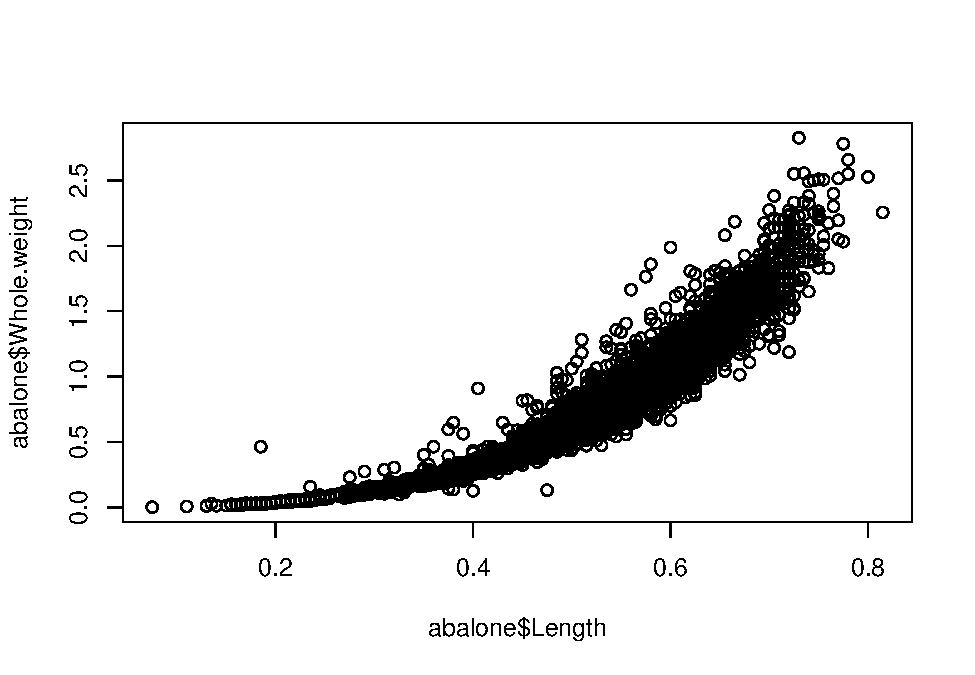
\includegraphics{_main_files/figure-latex/unnamed-chunk-35-1.pdf}

\begin{Shaded}
\begin{Highlighting}[]
\FunctionTok{plot}\NormalTok{(abalone}\SpecialCharTok{$}\NormalTok{Length, abalone}\SpecialCharTok{$}\NormalTok{Whole.weight, }\AttributeTok{col =}\NormalTok{ abalone}\SpecialCharTok{$}\NormalTok{Sex)}
\end{Highlighting}
\end{Shaded}

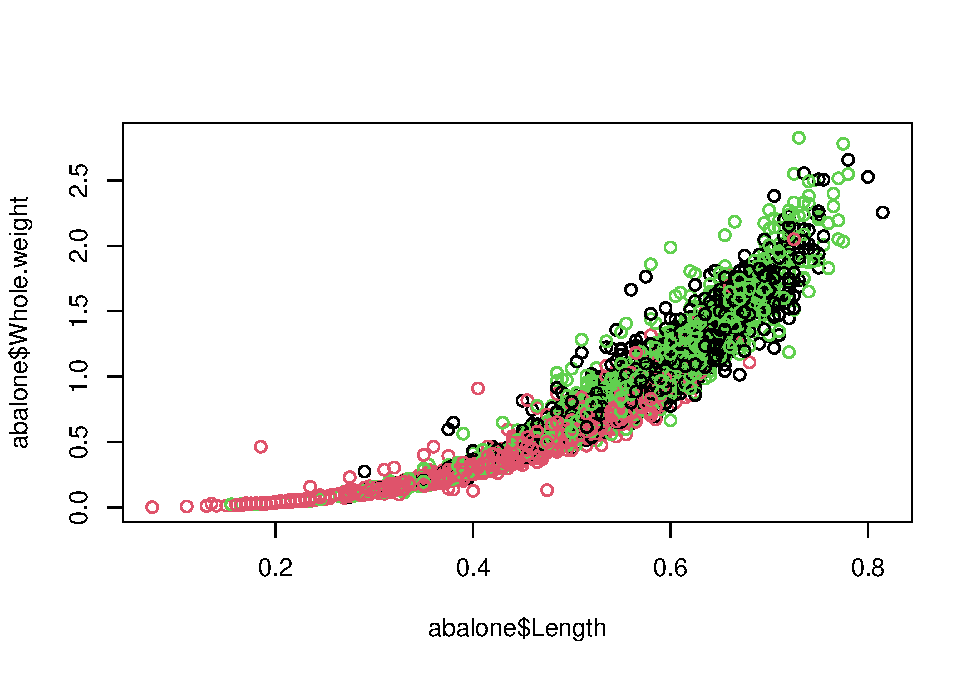
\includegraphics{_main_files/figure-latex/unnamed-chunk-36-1.pdf}

You cannot color on a column of categorical data if it is not a factor because each entry is considered unique, there are no shared characteristics between the observations.

It can be confusing to figure out which color corresponds to which category in base R.

\begin{Shaded}
\begin{Highlighting}[]
\FunctionTok{class}\NormalTok{(abalone}\SpecialCharTok{$}\NormalTok{Sex)}
\end{Highlighting}
\end{Shaded}

\begin{verbatim}
## [1] "factor"
\end{verbatim}

\begin{Shaded}
\begin{Highlighting}[]
\FunctionTok{levels}\NormalTok{(abalone}\SpecialCharTok{$}\NormalTok{Sex)}
\end{Highlighting}
\end{Shaded}

\begin{verbatim}
## [1] "F" "I" "M"
\end{verbatim}

Let's make a table to specify the color we want each level to be

\begin{Shaded}
\begin{Highlighting}[]
\FunctionTok{plot}\NormalTok{(abalone}\SpecialCharTok{$}\NormalTok{Length, abalone}\SpecialCharTok{$}\NormalTok{Whole.weight, }\AttributeTok{col=}\NormalTok{abalone}\SpecialCharTok{$}\NormalTok{Sex, }
     \AttributeTok{main =} \StringTok{"Abalone weight increases with length"}\NormalTok{, }
     \AttributeTok{xlab =} \StringTok{"Length (mm)"}\NormalTok{, }
     \AttributeTok{ylab =} \StringTok{"Whole weight (g)"}\NormalTok{)}

\FunctionTok{legend}\NormalTok{(}\AttributeTok{x=}\StringTok{"bottomright"}\NormalTok{, }
       \AttributeTok{legend =} \FunctionTok{levels}\NormalTok{(abalone}\SpecialCharTok{$}\NormalTok{Sex), }
       \AttributeTok{col =} \DecValTok{1}\SpecialCharTok{:}\DecValTok{3}\NormalTok{, }
       \AttributeTok{pch =} \DecValTok{5}
\NormalTok{       )}
\end{Highlighting}
\end{Shaded}

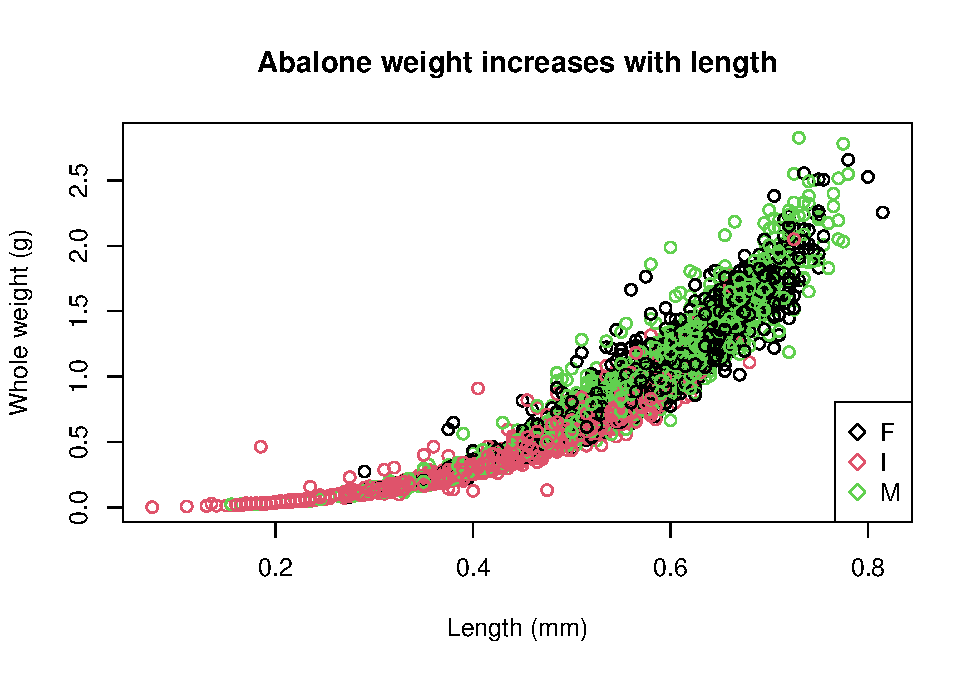
\includegraphics{_main_files/figure-latex/unnamed-chunk-38-1.pdf}

Base R plots use layers so the base \texttt{plot()} must be created first, before the \texttt{legend()} layer is added on top.

I stands for infant so it makes sense that they would be smaller in weight and length compared to the mature abalone.

Before we move on to the next type of plot, let's customize it a bit more by cleaning up the axis

\subsection{Scatterplot with ggplot}\label{scatterplot-with-ggplot}

\texttt{ggplot()} was created to support customizable and reproducible plots. The way that the \texttt{ggplot()} function accepts the data is much different from the base R \texttt{plot()} function.

The both columns of data must be in the same dataframe and specified in the \emph{data} parameter. Then, the x and y axis must be specified using the aesthetic \emph{aes} parameter. The base \texttt{ggplot()} call only holds the data, the geometry or format of the plot must be further specified by a separate call.

While commas \texttt{,} separate the parameters in a function, plus signs \texttt{+} are used to specify different layers of the plot.

This is the basic template for ggplots:

\begin{quote}
ggplot(data = , mapping = aes()) + ()
\end{quote}

\begin{Shaded}
\begin{Highlighting}[]
\FunctionTok{library}\NormalTok{(ggplot2)}
\end{Highlighting}
\end{Shaded}

A single continuous variable can be displayed using a histogram.

\begin{Shaded}
\begin{Highlighting}[]
\FunctionTok{ggplot}\NormalTok{(}\AttributeTok{data =}\NormalTok{ abalone, }\AttributeTok{mapping =} \FunctionTok{aes}\NormalTok{(}\AttributeTok{x=}\NormalTok{Length)) }\SpecialCharTok{+}
  \FunctionTok{geom\_histogram}\NormalTok{()}
\end{Highlighting}
\end{Shaded}

\begin{verbatim}
## `stat_bin()` using `bins = 30`. Pick better value with `binwidth`.
\end{verbatim}

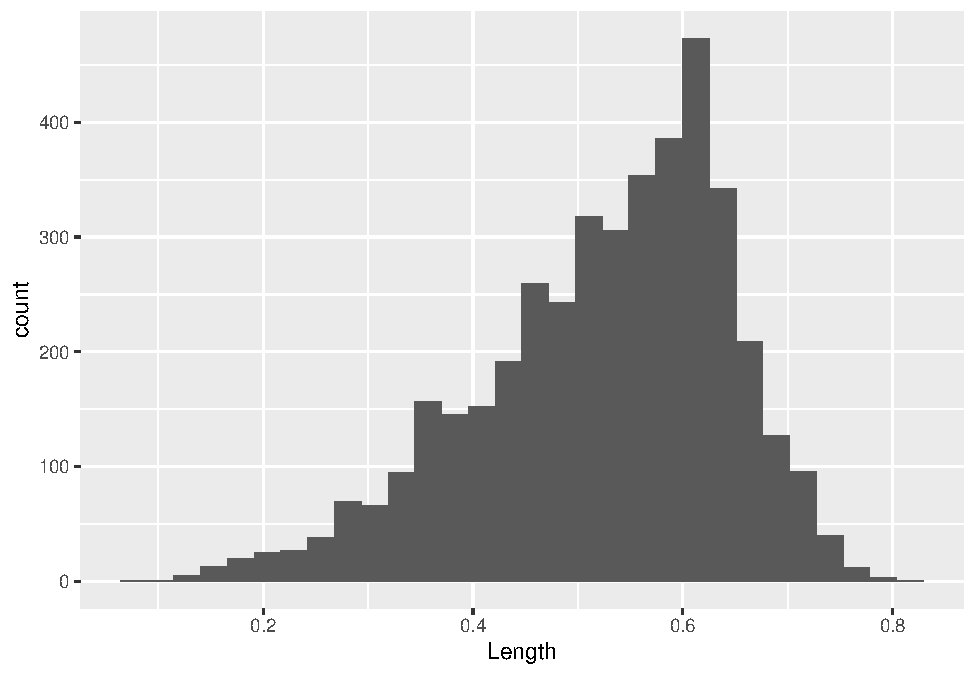
\includegraphics{_main_files/figure-latex/unnamed-chunk-43-1.pdf}

\begin{Shaded}
\begin{Highlighting}[]
\FunctionTok{nrow}\NormalTok{(abalone)}
\end{Highlighting}
\end{Shaded}

\begin{verbatim}
## [1] 4177
\end{verbatim}

Two continuous variables can be contrasted using a point or scatter plot.

\begin{Shaded}
\begin{Highlighting}[]
\FunctionTok{ggplot}\NormalTok{(abalone, }\FunctionTok{aes}\NormalTok{(}\AttributeTok{x =}\NormalTok{ Length, }\AttributeTok{y =}\NormalTok{ Whole.weight)) }\SpecialCharTok{+} 
  \FunctionTok{geom\_point}\NormalTok{()}
\end{Highlighting}
\end{Shaded}

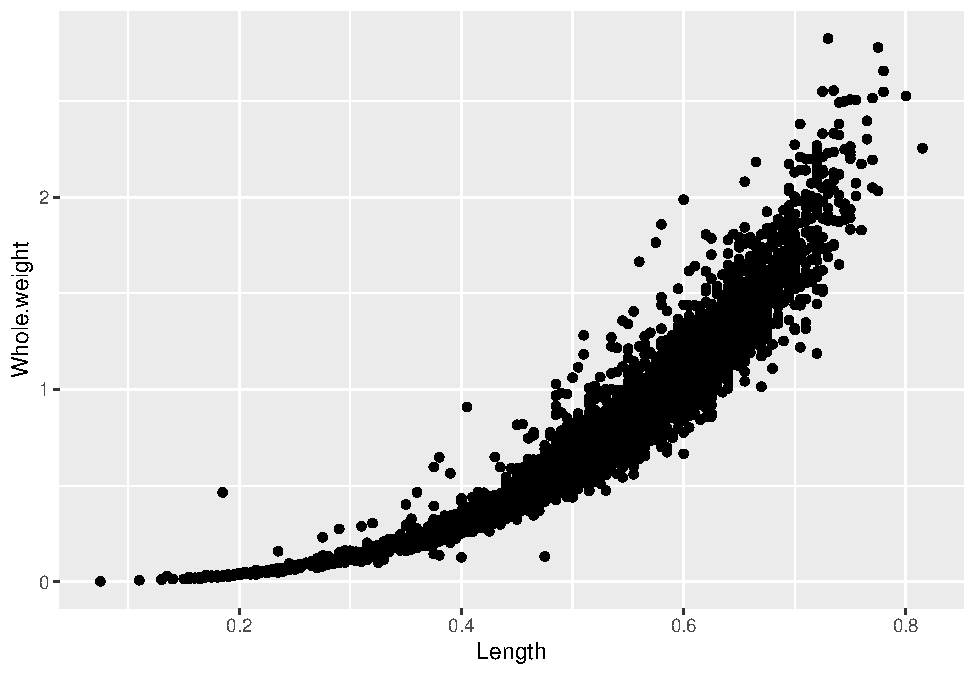
\includegraphics{_main_files/figure-latex/unnamed-chunk-44-1.pdf}

It is a lot simpler to add color to ggplots

\begin{Shaded}
\begin{Highlighting}[]
\FunctionTok{ggplot}\NormalTok{(abalone, }\FunctionTok{aes}\NormalTok{(}\AttributeTok{x =}\NormalTok{ Length, }\AttributeTok{y =}\NormalTok{ Whole.weight, }\AttributeTok{col =}\NormalTok{ Sex)) }\SpecialCharTok{+} 
  \FunctionTok{geom\_point}\NormalTok{()}
\end{Highlighting}
\end{Shaded}

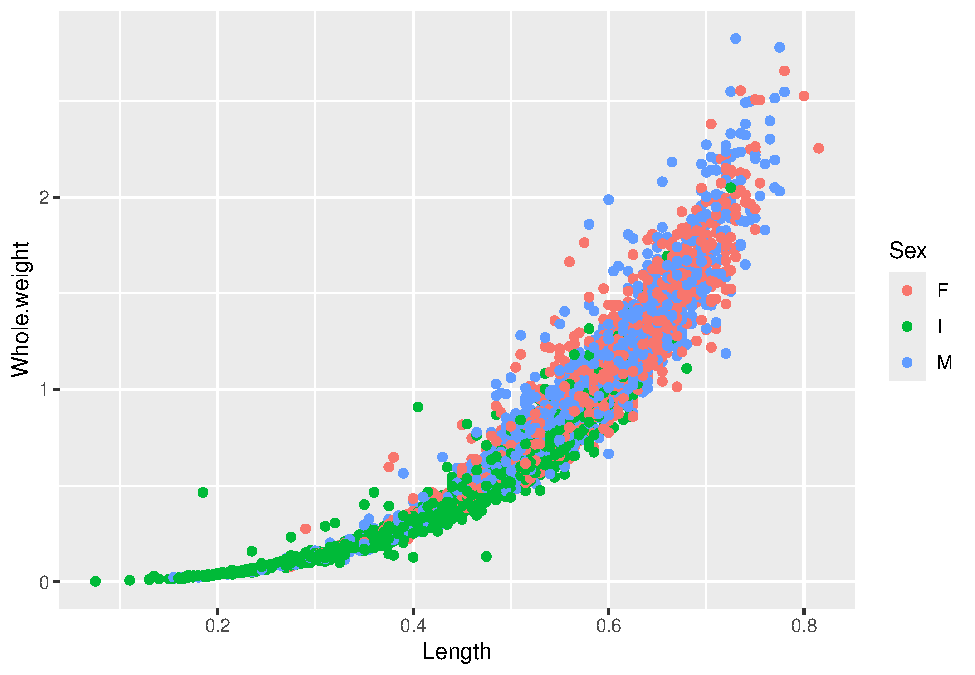
\includegraphics{_main_files/figure-latex/unnamed-chunk-45-1.pdf}

There's a lot of dots that are piling up on top of each other so we can change the alpha value to modify the transparency. Remember, you can always look up more information about each function using the \texttt{?} or looking online! No need to memorize everything!

\begin{Shaded}
\begin{Highlighting}[]
\FunctionTok{ggplot}\NormalTok{(abalone, }\FunctionTok{aes}\NormalTok{(}\AttributeTok{x =}\NormalTok{ Length, }\AttributeTok{y =}\NormalTok{ Whole.weight, }\AttributeTok{col =}\NormalTok{ Sex)) }\SpecialCharTok{+} 
  \FunctionTok{geom\_point}\NormalTok{(}\AttributeTok{alpha =} \FloatTok{0.3}\NormalTok{)}
\end{Highlighting}
\end{Shaded}

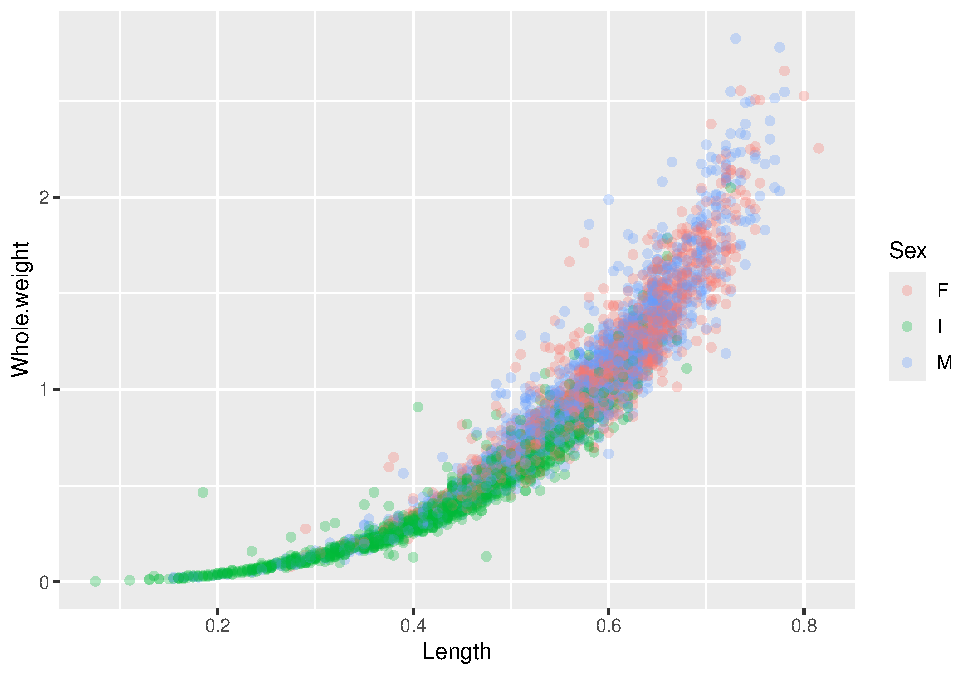
\includegraphics{_main_files/figure-latex/unnamed-chunk-46-1.pdf}

\subsubsection{Exercise}\label{exercise-2}

Create a plot to investigate the relationship between the shucked weight and the shell weight of ONLY adult abalone (exclude the infant abalones). Color the plot by Sex, do you notice any difference between the two?

\begin{Shaded}
\begin{Highlighting}[]
\NormalTok{abalone\_MF }\OtherTok{\textless{}{-}}\NormalTok{ abalone[abalone}\SpecialCharTok{$}\NormalTok{Sex }\SpecialCharTok{\%in\%} \FunctionTok{c}\NormalTok{(}\StringTok{"M"}\NormalTok{, }\StringTok{"F"}\NormalTok{), ]}

\FunctionTok{ggplot}\NormalTok{(abalone\_MF, }\FunctionTok{aes}\NormalTok{(}\AttributeTok{x=}\NormalTok{Shucked.weight, }\AttributeTok{y =}\NormalTok{ Shell.weight, }\AttributeTok{col =}\NormalTok{ Sex)) }\SpecialCharTok{+}
  \FunctionTok{geom\_point}\NormalTok{()}
\end{Highlighting}
\end{Shaded}

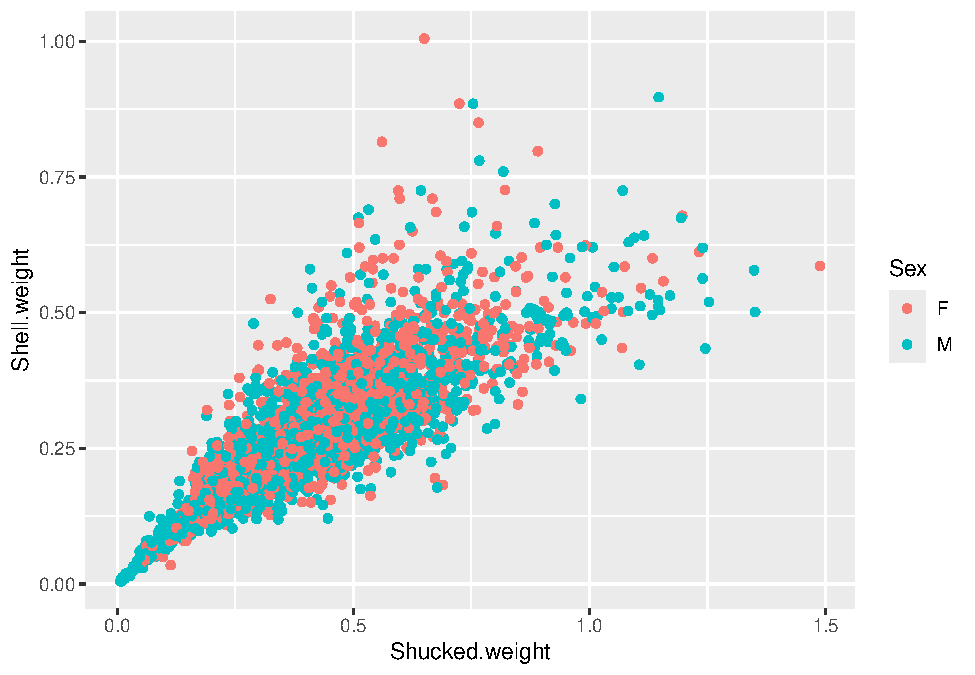
\includegraphics{_main_files/figure-latex/unnamed-chunk-47-1.pdf}

Let's take a closer look at categorical data. One categorical data can be displayed with a bar plot. This is helpful when we are looking to see if we have equal representation in each of the sample groups.

\begin{Shaded}
\begin{Highlighting}[]
\FunctionTok{ggplot}\NormalTok{(abalone, }\FunctionTok{aes}\NormalTok{(}\AttributeTok{x=}\NormalTok{ Sex, }\AttributeTok{fill =}\NormalTok{ Sex)) }\SpecialCharTok{+} 
  \FunctionTok{geom\_bar}\NormalTok{()}
\end{Highlighting}
\end{Shaded}

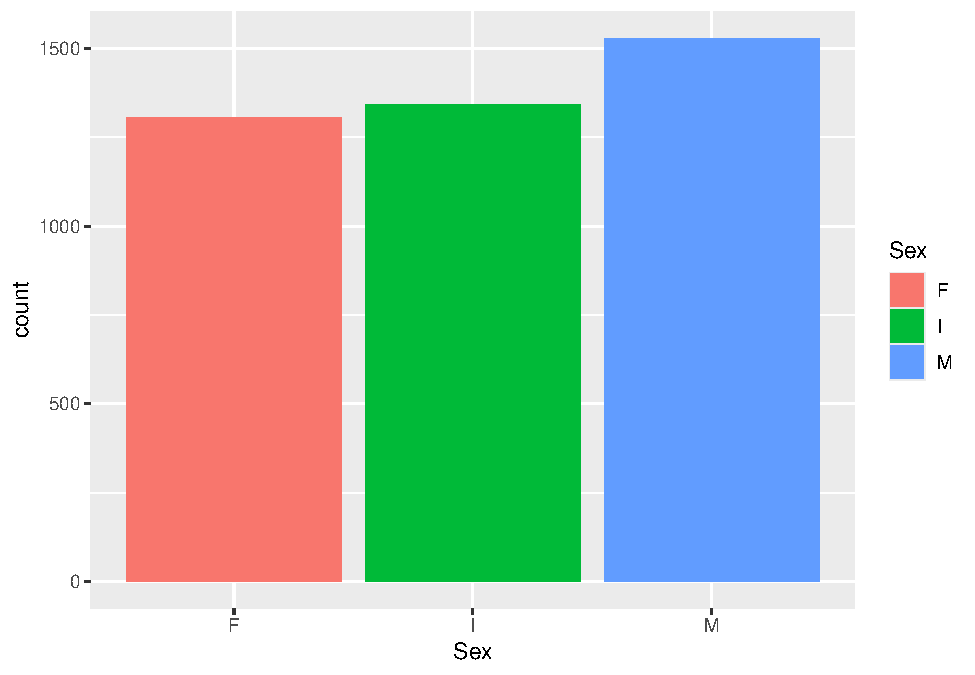
\includegraphics{_main_files/figure-latex/unnamed-chunk-48-1.pdf}

Bar plots can also be easily modified.

\begin{Shaded}
\begin{Highlighting}[]
\FunctionTok{ggplot}\NormalTok{(abalone, }\FunctionTok{aes}\NormalTok{(}\AttributeTok{x=}\NormalTok{ Sex, }\AttributeTok{fill =}\NormalTok{ Sex)) }\SpecialCharTok{+} 
  \FunctionTok{geom\_bar}\NormalTok{(}\AttributeTok{width =} \FloatTok{0.5}\NormalTok{) }\SpecialCharTok{+}
  \FunctionTok{coord\_flip}\NormalTok{()}
\end{Highlighting}
\end{Shaded}

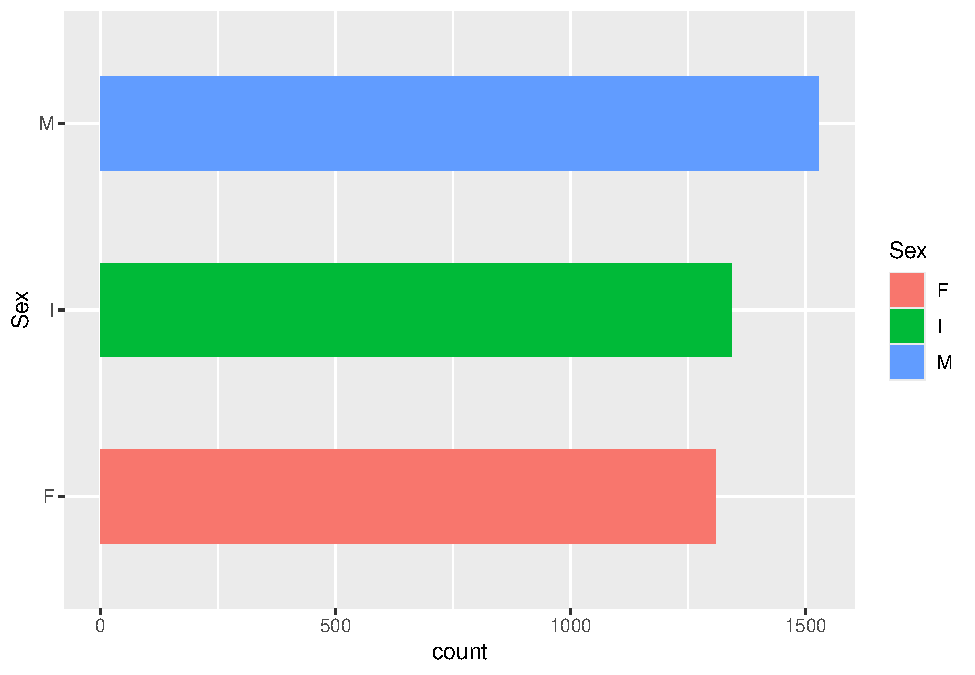
\includegraphics{_main_files/figure-latex/unnamed-chunk-49-1.pdf}

Lastly, boxplots are used to describe the relationship between a continuous and a categorical variable.

\begin{Shaded}
\begin{Highlighting}[]
\FunctionTok{ggplot}\NormalTok{(abalone, }\FunctionTok{aes}\NormalTok{(}\AttributeTok{x =}\NormalTok{ Sex, }\AttributeTok{y =}\NormalTok{ Whole.weight)) }\SpecialCharTok{+}
  \FunctionTok{geom\_boxplot}\NormalTok{()}
\end{Highlighting}
\end{Shaded}

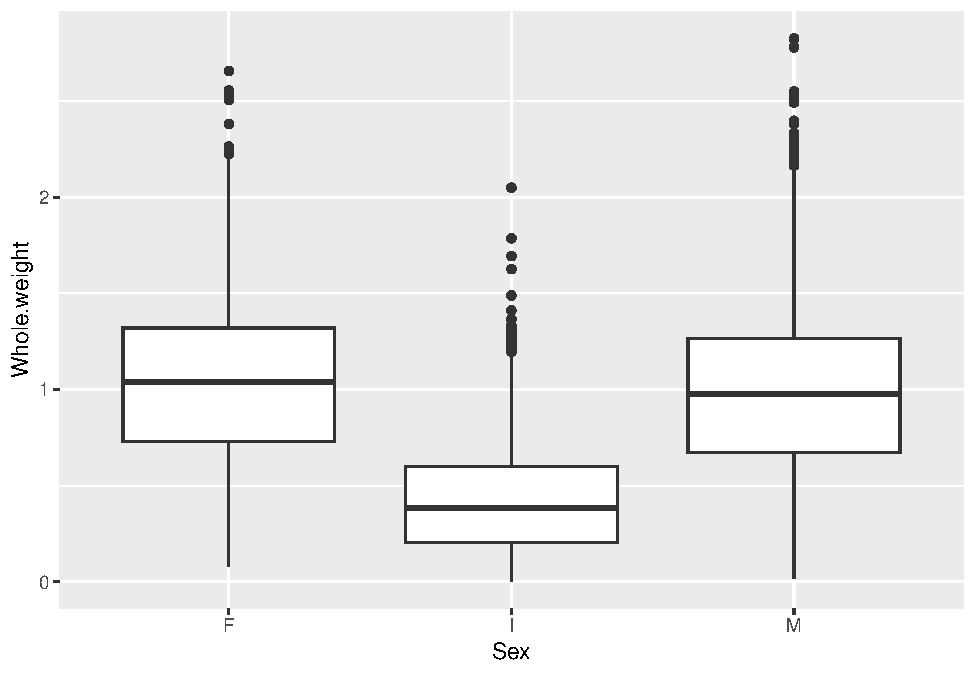
\includegraphics{_main_files/figure-latex/unnamed-chunk-50-1.pdf}

This more clearly shows that the weight distribution is comparable between the males and females. However, it would be clearer to have the F and M bars adjacent for comparison.

\begin{Shaded}
\begin{Highlighting}[]
\FunctionTok{levels}\NormalTok{(abalone}\SpecialCharTok{$}\NormalTok{Sex)}
\end{Highlighting}
\end{Shaded}

\begin{verbatim}
## [1] "F" "I" "M"
\end{verbatim}

\begin{Shaded}
\begin{Highlighting}[]
\NormalTok{abalone}\SpecialCharTok{$}\NormalTok{Sex }\OtherTok{\textless{}{-}} \FunctionTok{factor}\NormalTok{(abalone}\SpecialCharTok{$}\NormalTok{Sex, }\AttributeTok{levels =} \FunctionTok{c}\NormalTok{(}\StringTok{"I"}\NormalTok{, }\StringTok{"F"}\NormalTok{, }\StringTok{"M"}\NormalTok{))}

\FunctionTok{ggplot}\NormalTok{(abalone, }\FunctionTok{aes}\NormalTok{(}\AttributeTok{x =}\NormalTok{ Sex, }\AttributeTok{y =}\NormalTok{ Whole.weight)) }\SpecialCharTok{+}
  \FunctionTok{geom\_boxplot}\NormalTok{() }\SpecialCharTok{+} 
  \FunctionTok{theme\_classic}\NormalTok{()}
\end{Highlighting}
\end{Shaded}

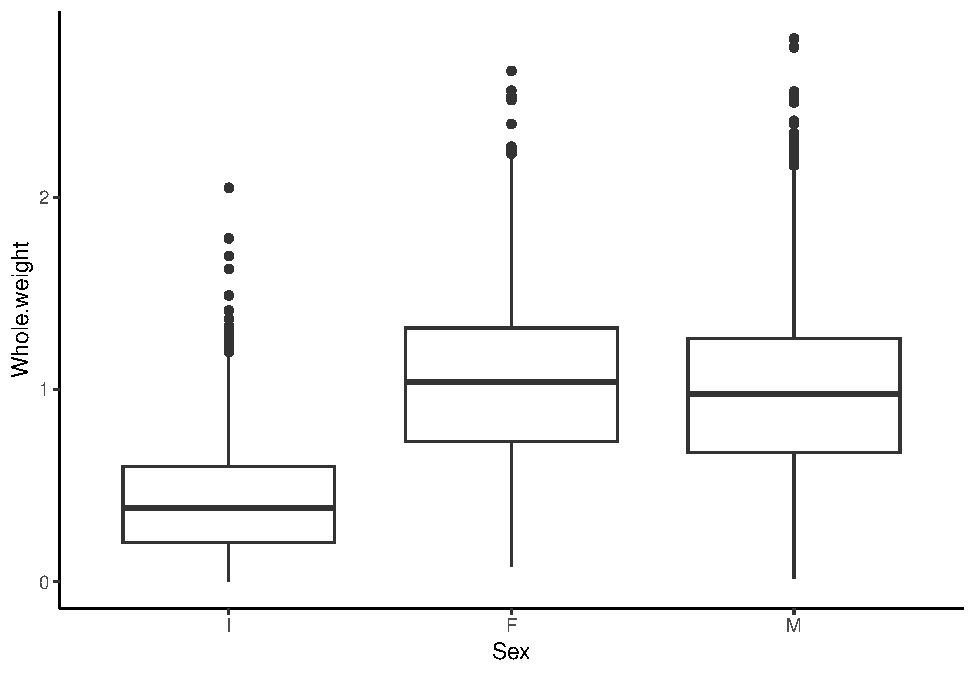
\includegraphics{_main_files/figure-latex/unnamed-chunk-51-1.pdf}

\subsection{Multi-panel Plots with ggplot}\label{multi-panel-plots-with-ggplot}

Plots can be saved as objects

\begin{Shaded}
\begin{Highlighting}[]
\NormalTok{p1 }\OtherTok{\textless{}{-}} \FunctionTok{ggplot}\NormalTok{(abalone\_MF, }\FunctionTok{aes}\NormalTok{(}\AttributeTok{x=}\NormalTok{Shucked.weight, }\AttributeTok{y =}\NormalTok{ Shell.weight, }\AttributeTok{col =}\NormalTok{ Sex)) }\SpecialCharTok{+}
  \FunctionTok{geom\_point}\NormalTok{()}

\NormalTok{p2 }\OtherTok{\textless{}{-}} \FunctionTok{ggplot}\NormalTok{(abalone, }\FunctionTok{aes}\NormalTok{(}\AttributeTok{x =}\NormalTok{ Sex, }\AttributeTok{y =}\NormalTok{ Whole.weight)) }\SpecialCharTok{+}
  \FunctionTok{geom\_boxplot}\NormalTok{() }\SpecialCharTok{+} 
  \FunctionTok{theme\_classic}\NormalTok{()}

\NormalTok{p1}
\end{Highlighting}
\end{Shaded}

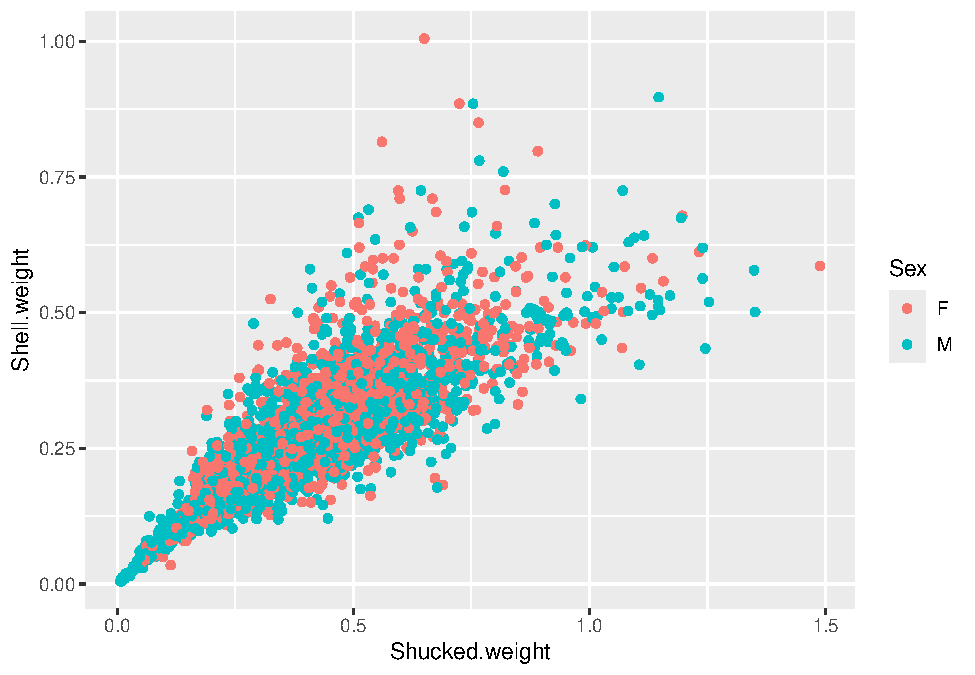
\includegraphics{_main_files/figure-latex/unnamed-chunk-52-1.pdf}
Rather than flipping between separating plots and stitching them together afterwards in a photo editor, we can arrange them into a figure panel all together in R

\begin{Shaded}
\begin{Highlighting}[]
\CommentTok{\#install.packages("cowplot")}
\FunctionTok{library}\NormalTok{(cowplot)}
\end{Highlighting}
\end{Shaded}

\begin{verbatim}
## 
## Attaching package: 'cowplot'
\end{verbatim}

\begin{verbatim}
## The following object is masked from 'package:lubridate':
## 
##     stamp
\end{verbatim}

\begin{Shaded}
\begin{Highlighting}[]
\FunctionTok{plot\_grid}\NormalTok{(p1, p2)}
\end{Highlighting}
\end{Shaded}

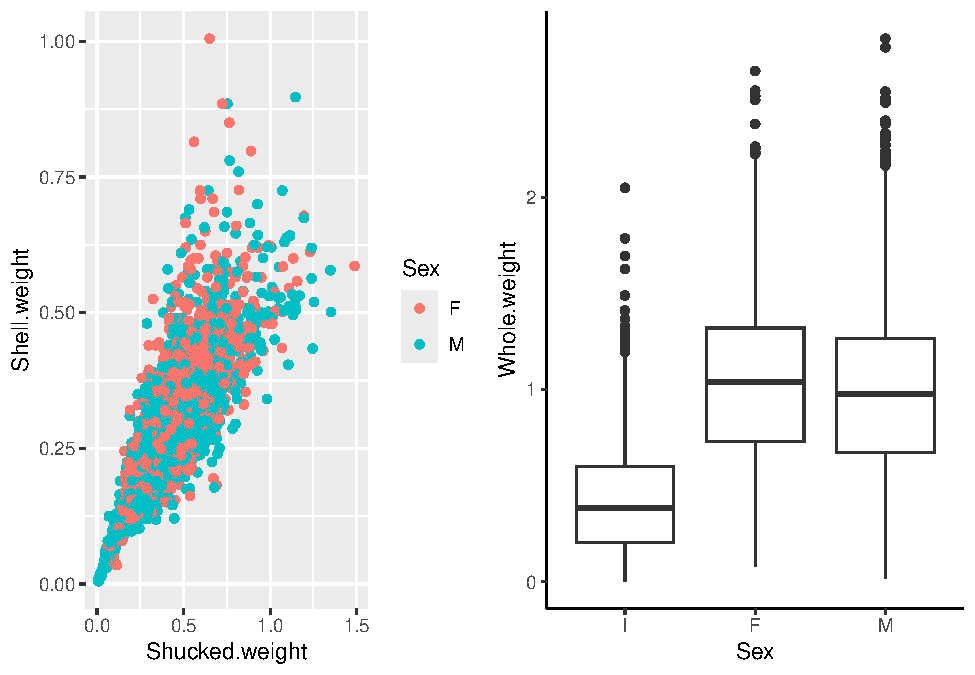
\includegraphics{_main_files/figure-latex/unnamed-chunk-53-1.pdf}
Let's clean this up a bit

\begin{Shaded}
\begin{Highlighting}[]
\NormalTok{top\_row }\OtherTok{\textless{}{-}} \FunctionTok{plot\_grid}\NormalTok{(p1 }\SpecialCharTok{+} \FunctionTok{theme\_classic}\NormalTok{(), }
\NormalTok{          p2, }
          \AttributeTok{labels =} \FunctionTok{c}\NormalTok{(}\StringTok{"A"}\NormalTok{, }\StringTok{"B"}\NormalTok{), }
          \AttributeTok{label\_size =} \DecValTok{20}\NormalTok{)}

\NormalTok{top\_row}
\end{Highlighting}
\end{Shaded}

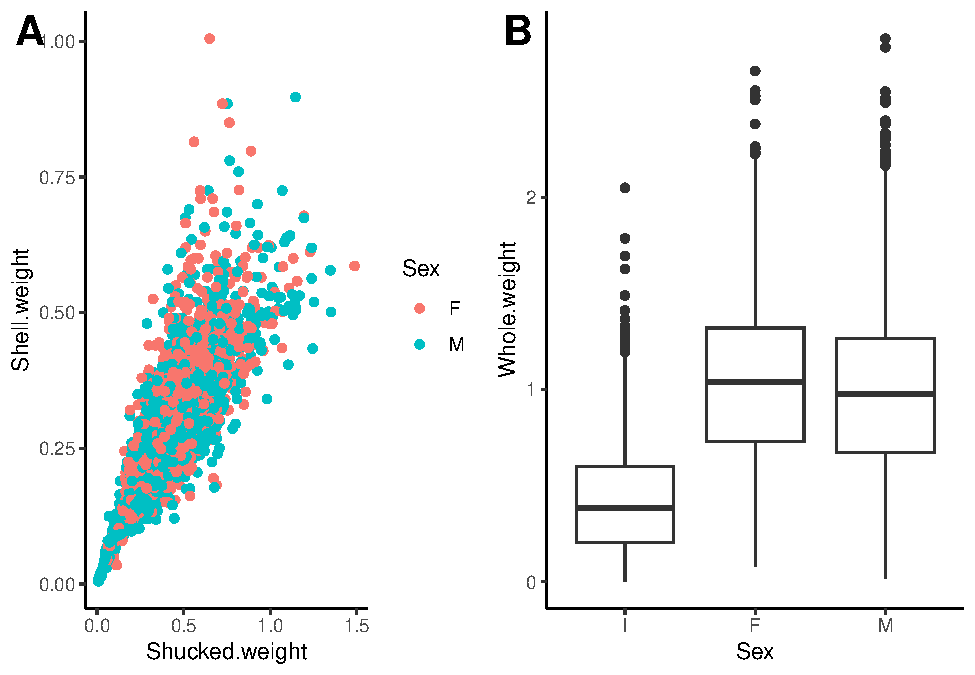
\includegraphics{_main_files/figure-latex/unnamed-chunk-54-1.pdf}
Adding a third plot to play around with the distribution between panels

We want p1 to be larger by itself in the top row and then p2 and p3 split in the bottom row.

\begin{Shaded}
\begin{Highlighting}[]
\NormalTok{p3 }\OtherTok{\textless{}{-}} \FunctionTok{ggplot}\NormalTok{(abalone, }\FunctionTok{aes}\NormalTok{(Sex)) }\SpecialCharTok{+} \FunctionTok{geom\_bar}\NormalTok{()}

\FunctionTok{plot\_grid}\NormalTok{(top\_row, p3, }\AttributeTok{ncol=}\DecValTok{1}\NormalTok{, }
          \AttributeTok{labels =} \FunctionTok{c}\NormalTok{(}\StringTok{""}\NormalTok{, }\StringTok{"C"}\NormalTok{), }
          \AttributeTok{label\_size =} \DecValTok{20}\NormalTok{)}
\end{Highlighting}
\end{Shaded}

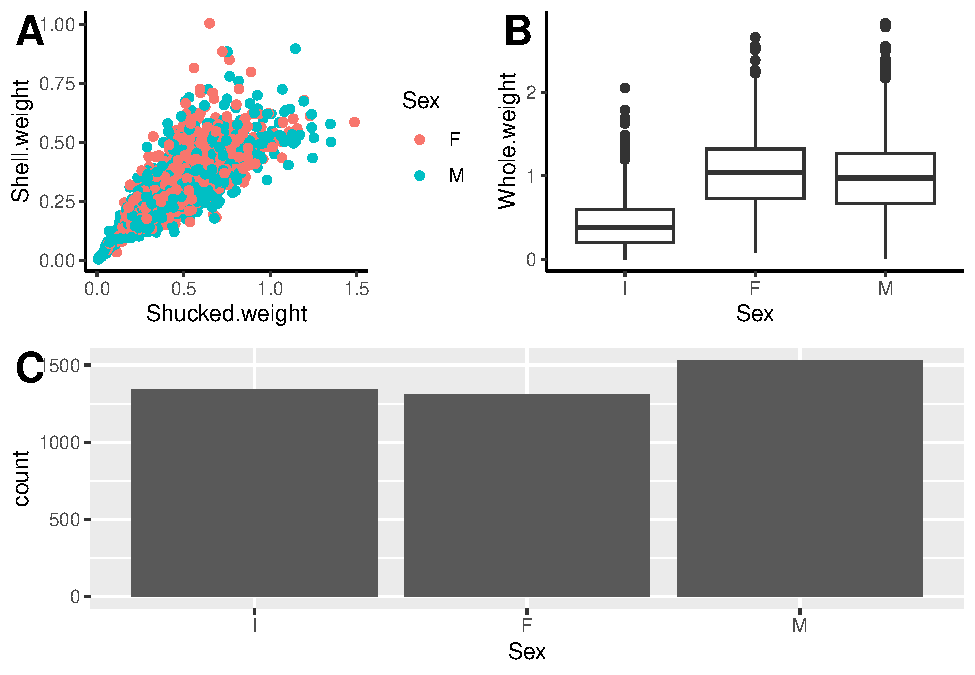
\includegraphics{_main_files/figure-latex/unnamed-chunk-55-1.pdf}

\subsection{Exporting plots}\label{exporting-plots}

\begin{Shaded}
\begin{Highlighting}[]
\FunctionTok{getwd}\NormalTok{()}
\end{Highlighting}
\end{Shaded}

\begin{verbatim}
## [1] "/Users/clin/Documents/CBWGitHub/INR_2024"
\end{verbatim}

\begin{Shaded}
\begin{Highlighting}[]
\FunctionTok{png}\NormalTok{(}\AttributeTok{file =} \StringTok{"INR\_fig1.png"}\NormalTok{, }\AttributeTok{bg =} \StringTok{"transparent"}\NormalTok{)}
\NormalTok{top\_row}
\FunctionTok{dev.off}\NormalTok{()}
\end{Highlighting}
\end{Shaded}

\begin{verbatim}
## pdf 
##   2
\end{verbatim}

\subsection{Day 1 Project}\label{day-1-project}

For this mini guided project, we will be working with a dataset quantifying water quality that is publicly available at: \url{https://www.kaggle.com/datasets/adityakadiwal/water-potability?resource=download}

Here is some description of the data:

Access to safe drinking-water is essential to health, a basic human right and a component of effective policy for health protection. This is important as a health and development issue at a national, regional and local level. In some regions, it has been shown that investments in water supply and sanitation can yield a net economic benefit, since the reductions in adverse health effects and health care costs outweigh the costs of undertaking the interventions.
Content

The water\_potability.csv file contains water quality metrics for 3276 different water bodies. More information about each of the columns can be found in the link above

pH value
Hardness
Solids (Total dissolved solids - TDS)
Chloramines
Sulfate
Conductivity
Organic\_carbon
Trihalomethanes
Turbidity
Potability

Insert a code chunk underneath each step to carry out the instruction.

\begin{enumerate}
\def\labelenumi{\arabic{enumi}.}
\item
  Read in the ``water\_potability.csv'' data into an object called data Check the object you created by printing out the first 10 rows and applying the summary function.
\item
  Notice that the pH column contains a couple hundred NA values. NA are special values in R (like how ``pi'' is preset to a value of 3.14159\ldots) to indicate that there is missing data, or it is not available. There are also some NAs in the Sulfate and Trihalomethanes columns.
\end{enumerate}

Create new object called water\_df that only contains complete observations.

Take a look at the function called \texttt{na.omit()}. In most cases, someone's already done what you've wanted to do so there may already be code or functions that you can adapt and use!

\begin{enumerate}
\def\labelenumi{\arabic{enumi}.}
\setcounter{enumi}{2}
\tightlist
\item
  The Potability column has two possible values: 1 means Potable and 0 means Not potable.
\end{enumerate}

It is read in by default as a character vector. Convert this column to a factor.

\begin{enumerate}
\def\labelenumi{\arabic{enumi}.}
\setcounter{enumi}{3}
\tightlist
\item
  WHO has recommended maximum permissible limit of pH in drinking water from 6.5 to 8.5.
\end{enumerate}

Create a new column within the \texttt{water\_df} object called \texttt{ph\_category} in which:

\begin{itemize}
\tightlist
\item
  Observations with a pH less than 6.5 have a value of \texttt{acidic} in the \texttt{ph\_category}
\item
  Observations with a pH betwee 6.5 - 8.5 have a value of \texttt{permissible} in the \texttt{ph\_category}
\item
  Observations with a pH greater than 8.5 have a value of \texttt{basic} in the \texttt{ph\_category}
\end{itemize}

There are multiple ways to do this, give it a go! You can't break the object - if you ever feel like you need a reset, you can always repeat step 1 to read in the object again.

Use \texttt{table()} or \texttt{summary()} to check the values in the \texttt{ph\_category} column

\begin{enumerate}
\def\labelenumi{\arabic{enumi}.}
\setcounter{enumi}{4}
\tightlist
\item
  Create a plot to double check if the annotations in the \texttt{ph\_category} column were applied correctly. Make sure to represent both the \texttt{ph} and \texttt{ph\_category} columns.
\end{enumerate}

You're welcome to use base R or ggplot functions. There are multiple ways of representing these two columns. ggplot is slightly preferred because of its increased customization so it's good to get some practice with it!

\begin{enumerate}
\def\labelenumi{\arabic{enumi}.}
\setcounter{enumi}{5}
\tightlist
\item
  The levels of sulfates and water hardness cause by salts should be minimized in order to be safe for consumption.
\end{enumerate}

Create a plot with the level of water hardness on the x axis and sulphate on the y axis colored by the Potability column.

Try applying the \texttt{facet\_grid()} layer to the plot in order to group the plots by a factor. Make sure to use the \texttt{\textasciitilde{}} before the column name!

The data is quite messy so don't worry if the results do not separate as much as you would like - real data is messy!

Congratulations! You have completed Lab 1!

\chapter{Day 2}\label{day-2}

\section{Lab}\label{lab-1}

\subsection{Project Review}\label{project-review}

For this mini guided project, we will be working with a dataset quantifying water quality that is publicly available at: \url{https://www.kaggle.com/datasets/adityakadiwal/water-potability?resource=download}

Here is some description of the data:

Access to safe drinking-water is essential to health, a basic human right and a component of effective policy for health protection. This is important as a health and development issue at a national, regional and local level. In some regions, it has been shown that investments in water supply and sanitation can yield a net economic benefit, since the reductions in adverse health effects and health care costs outweigh the costs of undertaking the interventions.
Content

The water\_potability.csv file contains water quality metrics for 3276 different water bodies. More information about each of the columns can be found in the link above

pH value
Hardness
Solids (Total dissolved solids - TDS)
Chloramines
Sulfate
Conductivity
Organic\_carbon
Trihalomethanes
Turbidity
Potability

Insert a code chunk underneath each step to carry out the instruction.

\begin{enumerate}
\def\labelenumi{\arabic{enumi}.}
\tightlist
\item
  Read in the ``water\_potability.csv'' data into an object called data Check the object you created by printing out the first 10 rows and applying the summary function.
\end{enumerate}

\begin{Shaded}
\begin{Highlighting}[]
\NormalTok{data }\OtherTok{\textless{}{-}} \FunctionTok{read.csv}\NormalTok{(}\StringTok{"../INR{-}2024/datasets/water\_potability.csv"}\NormalTok{)}

\FunctionTok{head}\NormalTok{(data, }\AttributeTok{n=}\DecValTok{10}\NormalTok{)}
\end{Highlighting}
\end{Shaded}

\begin{verbatim}
##           ph Hardness   Solids Chloramines  Sulfate Conductivity Organic_carbon
## 1         NA 204.8905 20791.32    7.300212 368.5164     564.3087      10.379783
## 2   3.716080 129.4229 18630.06    6.635246       NA     592.8854      15.180013
## 3   8.099124 224.2363 19909.54    9.275884       NA     418.6062      16.868637
## 4   8.316766 214.3734 22018.42    8.059332 356.8861     363.2665      18.436524
## 5   9.092223 181.1015 17978.99    6.546600 310.1357     398.4108      11.558279
## 6   5.584087 188.3133 28748.69    7.544869 326.6784     280.4679       8.399735
## 7  10.223862 248.0717 28749.72    7.513408 393.6634     283.6516      13.789695
## 8   8.635849 203.3615 13672.09    4.563009 303.3098     474.6076      12.363817
## 9         NA 118.9886 14285.58    7.804174 268.6469     389.3756      12.706049
## 10 11.180284 227.2315 25484.51    9.077200 404.0416     563.8855      17.927806
##    Trihalomethanes Turbidity Potability
## 1         86.99097  2.963135          0
## 2         56.32908  4.500656          0
## 3         66.42009  3.055934          0
## 4        100.34167  4.628771          0
## 5         31.99799  4.075075          0
## 6         54.91786  2.559708          0
## 7         84.60356  2.672989          0
## 8         62.79831  4.401425          0
## 9         53.92885  3.595017          0
## 10        71.97660  4.370562          0
\end{verbatim}

\begin{Shaded}
\begin{Highlighting}[]
\NormalTok{data[}\DecValTok{1}\SpecialCharTok{:}\DecValTok{10}\NormalTok{, ]}
\end{Highlighting}
\end{Shaded}

\begin{verbatim}
##           ph Hardness   Solids Chloramines  Sulfate Conductivity Organic_carbon
## 1         NA 204.8905 20791.32    7.300212 368.5164     564.3087      10.379783
## 2   3.716080 129.4229 18630.06    6.635246       NA     592.8854      15.180013
## 3   8.099124 224.2363 19909.54    9.275884       NA     418.6062      16.868637
## 4   8.316766 214.3734 22018.42    8.059332 356.8861     363.2665      18.436524
## 5   9.092223 181.1015 17978.99    6.546600 310.1357     398.4108      11.558279
## 6   5.584087 188.3133 28748.69    7.544869 326.6784     280.4679       8.399735
## 7  10.223862 248.0717 28749.72    7.513408 393.6634     283.6516      13.789695
## 8   8.635849 203.3615 13672.09    4.563009 303.3098     474.6076      12.363817
## 9         NA 118.9886 14285.58    7.804174 268.6469     389.3756      12.706049
## 10 11.180284 227.2315 25484.51    9.077200 404.0416     563.8855      17.927806
##    Trihalomethanes Turbidity Potability
## 1         86.99097  2.963135          0
## 2         56.32908  4.500656          0
## 3         66.42009  3.055934          0
## 4        100.34167  4.628771          0
## 5         31.99799  4.075075          0
## 6         54.91786  2.559708          0
## 7         84.60356  2.672989          0
## 8         62.79831  4.401425          0
## 9         53.92885  3.595017          0
## 10        71.97660  4.370562          0
\end{verbatim}

\begin{enumerate}
\def\labelenumi{\arabic{enumi}.}
\setcounter{enumi}{1}
\tightlist
\item
  Notice that the pH column contains a couple hundred NA values. NA are special values in R (like how ``pi'' is preset to a value of 3.14159\ldots) to indicate that there is missing data, or it is not available. There are also some NAs in the Sulfate and Trihalomethanes columns.
\end{enumerate}

Create new object called water\_df that only contains complete observations.

Take a look at the function called \texttt{na.omit()}. In most cases, someone's already done what you've wanted to do so there may already be code or functions that you can adapt and use!

\begin{Shaded}
\begin{Highlighting}[]
\NormalTok{water\_df }\OtherTok{\textless{}{-}} \FunctionTok{na.omit}\NormalTok{(data)}
\FunctionTok{summary}\NormalTok{(data)}
\end{Highlighting}
\end{Shaded}

\begin{verbatim}
##        ph            Hardness          Solids         Chloramines    
##  Min.   : 0.000   Min.   : 47.43   Min.   :  320.9   Min.   : 0.352  
##  1st Qu.: 6.093   1st Qu.:176.85   1st Qu.:15666.7   1st Qu.: 6.127  
##  Median : 7.037   Median :196.97   Median :20927.8   Median : 7.130  
##  Mean   : 7.081   Mean   :196.37   Mean   :22014.1   Mean   : 7.122  
##  3rd Qu.: 8.062   3rd Qu.:216.67   3rd Qu.:27332.8   3rd Qu.: 8.115  
##  Max.   :14.000   Max.   :323.12   Max.   :61227.2   Max.   :13.127  
##  NA's   :491                                                         
##     Sulfate       Conductivity   Organic_carbon  Trihalomethanes  
##  Min.   :129.0   Min.   :181.5   Min.   : 2.20   Min.   :  0.738  
##  1st Qu.:307.7   1st Qu.:365.7   1st Qu.:12.07   1st Qu.: 55.845  
##  Median :333.1   Median :421.9   Median :14.22   Median : 66.622  
##  Mean   :333.8   Mean   :426.2   Mean   :14.28   Mean   : 66.396  
##  3rd Qu.:360.0   3rd Qu.:481.8   3rd Qu.:16.56   3rd Qu.: 77.337  
##  Max.   :481.0   Max.   :753.3   Max.   :28.30   Max.   :124.000  
##  NA's   :781                                     NA's   :162      
##    Turbidity       Potability    
##  Min.   :1.450   Min.   :0.0000  
##  1st Qu.:3.440   1st Qu.:0.0000  
##  Median :3.955   Median :0.0000  
##  Mean   :3.967   Mean   :0.3901  
##  3rd Qu.:4.500   3rd Qu.:1.0000  
##  Max.   :6.739   Max.   :1.0000  
## 
\end{verbatim}

\begin{Shaded}
\begin{Highlighting}[]
\FunctionTok{summary}\NormalTok{(water\_df)}
\end{Highlighting}
\end{Shaded}

\begin{verbatim}
##        ph             Hardness          Solids         Chloramines    
##  Min.   : 0.2275   Min.   : 73.49   Min.   :  320.9   Min.   : 1.391  
##  1st Qu.: 6.0897   1st Qu.:176.74   1st Qu.:15615.7   1st Qu.: 6.139  
##  Median : 7.0273   Median :197.19   Median :20933.5   Median : 7.144  
##  Mean   : 7.0860   Mean   :195.97   Mean   :21917.4   Mean   : 7.134  
##  3rd Qu.: 8.0530   3rd Qu.:216.44   3rd Qu.:27182.6   3rd Qu.: 8.110  
##  Max.   :14.0000   Max.   :317.34   Max.   :56488.7   Max.   :13.127  
##     Sulfate       Conductivity   Organic_carbon  Trihalomethanes  
##  Min.   :129.0   Min.   :201.6   Min.   : 2.20   Min.   :  8.577  
##  1st Qu.:307.6   1st Qu.:366.7   1st Qu.:12.12   1st Qu.: 55.953  
##  Median :332.2   Median :423.5   Median :14.32   Median : 66.542  
##  Mean   :333.2   Mean   :426.5   Mean   :14.36   Mean   : 66.401  
##  3rd Qu.:359.3   3rd Qu.:482.4   3rd Qu.:16.68   3rd Qu.: 77.292  
##  Max.   :481.0   Max.   :753.3   Max.   :27.01   Max.   :124.000  
##    Turbidity       Potability    
##  Min.   :1.450   Min.   :0.0000  
##  1st Qu.:3.443   1st Qu.:0.0000  
##  Median :3.968   Median :0.0000  
##  Mean   :3.970   Mean   :0.4033  
##  3rd Qu.:4.514   3rd Qu.:1.0000  
##  Max.   :6.495   Max.   :1.0000
\end{verbatim}

\begin{Shaded}
\begin{Highlighting}[]
\FunctionTok{dim}\NormalTok{(data)}
\end{Highlighting}
\end{Shaded}

\begin{verbatim}
## [1] 3276   10
\end{verbatim}

\begin{Shaded}
\begin{Highlighting}[]
\FunctionTok{dim}\NormalTok{(water\_df)}
\end{Highlighting}
\end{Shaded}

\begin{verbatim}
## [1] 2011   10
\end{verbatim}

\begin{enumerate}
\def\labelenumi{\arabic{enumi}.}
\setcounter{enumi}{2}
\tightlist
\item
  The Potability column has two possible values: 1 means Potable and 0 means Not potable.
\end{enumerate}

It is read in by default as a character vector. Convert this column to a factor.

\begin{Shaded}
\begin{Highlighting}[]
\NormalTok{water\_df}\SpecialCharTok{$}\NormalTok{Potability }\OtherTok{\textless{}{-}} \FunctionTok{as.factor}\NormalTok{(water\_df}\SpecialCharTok{$}\NormalTok{Potability)}
\FunctionTok{head}\NormalTok{(water\_df)}
\end{Highlighting}
\end{Shaded}

\begin{verbatim}
##           ph Hardness   Solids Chloramines  Sulfate Conductivity Organic_carbon
## 4   8.316766 214.3734 22018.42    8.059332 356.8861     363.2665      18.436524
## 5   9.092223 181.1015 17978.99    6.546600 310.1357     398.4108      11.558279
## 6   5.584087 188.3133 28748.69    7.544869 326.6784     280.4679       8.399735
## 7  10.223862 248.0717 28749.72    7.513408 393.6634     283.6516      13.789695
## 8   8.635849 203.3615 13672.09    4.563009 303.3098     474.6076      12.363817
## 10 11.180284 227.2315 25484.51    9.077200 404.0416     563.8855      17.927806
##    Trihalomethanes Turbidity Potability
## 4        100.34167  4.628771          0
## 5         31.99799  4.075075          0
## 6         54.91786  2.559708          0
## 7         84.60356  2.672989          0
## 8         62.79831  4.401425          0
## 10        71.97660  4.370562          0
\end{verbatim}

\begin{Shaded}
\begin{Highlighting}[]
\FunctionTok{table}\NormalTok{(water\_df}\SpecialCharTok{$}\NormalTok{Potability)}
\end{Highlighting}
\end{Shaded}

\begin{verbatim}
## 
##    0    1 
## 1200  811
\end{verbatim}

\begin{enumerate}
\def\labelenumi{\arabic{enumi}.}
\setcounter{enumi}{3}
\tightlist
\item
  WHO has recommended maximum permissible limit of pH in drinking water from 6.5 to 8.5.
\end{enumerate}

Create a new column within the \texttt{water\_df} object called \texttt{ph\_category} in which:

\begin{itemize}
\tightlist
\item
  Observations with a pH less than 6.5 have a value of \texttt{acidic} in the \texttt{ph\_category}
\item
  Observations with a pH betwee 6.5 - 8.5 have a value of \texttt{permissible} in the \texttt{ph\_category}
\item
  Observations with a pH greater than 8.5 have a value of \texttt{basic} in the \texttt{ph\_category}
\end{itemize}

There are multiple ways to do this, give it a go! You can't break the object - if you ever feel like you need a reset, you can always repeat step 1 to read in the object again.

Use \texttt{table()} or \texttt{summary()} to check the values in the \texttt{ph\_category} column

\begin{Shaded}
\begin{Highlighting}[]
\NormalTok{water\_df}\SpecialCharTok{$}\NormalTok{ph\_category }\OtherTok{\textless{}{-}} \StringTok{"permissible"}

\NormalTok{water\_df}\SpecialCharTok{$}\NormalTok{ph\_category[water\_df}\SpecialCharTok{$}\NormalTok{ph }\SpecialCharTok{\textless{}} \FloatTok{6.5}\NormalTok{] }\OtherTok{\textless{}{-}} \StringTok{"acidic"} 

\NormalTok{water\_df}\SpecialCharTok{$}\NormalTok{ph\_category[water\_df}\SpecialCharTok{$}\NormalTok{ph }\SpecialCharTok{\textgreater{}} \FloatTok{8.5}\NormalTok{] }\OtherTok{\textless{}{-}} \StringTok{"basic"}

\FunctionTok{table}\NormalTok{(water\_df}\SpecialCharTok{$}\NormalTok{ph\_category)}
\end{Highlighting}
\end{Shaded}

\begin{verbatim}
## 
##      acidic       basic permissible 
##         692         358         961
\end{verbatim}

\begin{Shaded}
\begin{Highlighting}[]
\FunctionTok{nrow}\NormalTok{(water\_df[water\_df}\SpecialCharTok{$}\NormalTok{ph }\SpecialCharTok{\textless{}}\FloatTok{6.5}\NormalTok{, ])}
\end{Highlighting}
\end{Shaded}

\begin{verbatim}
## [1] 692
\end{verbatim}

\begin{enumerate}
\def\labelenumi{\arabic{enumi}.}
\setcounter{enumi}{4}
\tightlist
\item
  Create a plot to double check if the annotations in the \texttt{ph\_category} column were applied correctly. Make sure to represent both the \texttt{ph} and \texttt{ph\_category} columns.
\end{enumerate}

You're welcome to use base R or ggplot functions. There are multiple ways of representing these two columns. ggplot is slightly preferred because of its increased customization so it's good to get some practice with it!

\begin{Shaded}
\begin{Highlighting}[]
\FunctionTok{library}\NormalTok{(ggplot2)}
\FunctionTok{ggplot}\NormalTok{(water\_df, }\FunctionTok{aes}\NormalTok{(}\AttributeTok{x=}\NormalTok{ph\_category, }\AttributeTok{y=}\NormalTok{ph)) }\SpecialCharTok{+} 
  \FunctionTok{geom\_boxplot}\NormalTok{()}
\end{Highlighting}
\end{Shaded}

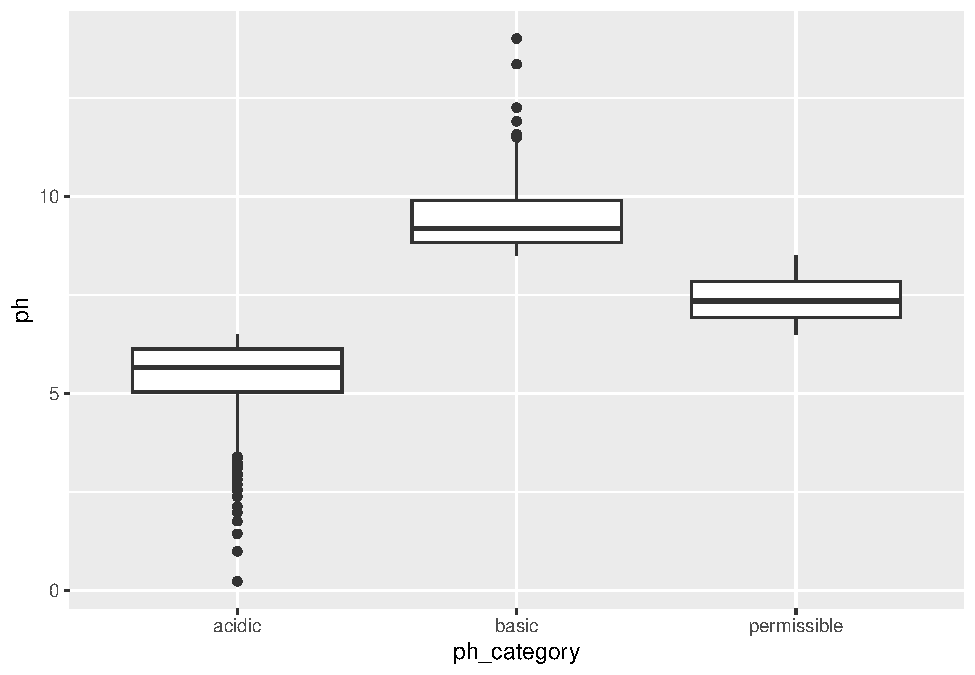
\includegraphics{_main_files/figure-latex/unnamed-chunk-63-1.pdf}

\begin{enumerate}
\def\labelenumi{\arabic{enumi}.}
\setcounter{enumi}{5}
\tightlist
\item
  The levels of sulfates and water hardness cause by salts should be minimized in order to be safe for consumption.
\end{enumerate}

Create a plot with the level of water hardness on the x axis and sulphate on the y axis colored by the Potability column.

Try applying the \texttt{facet\_grid()} layer to the plot in order to group the plots by a factor. Make sure to use the \texttt{\textasciitilde{}} before the column name!

The data is quite messy so don't worry if the results do not separate as much as you would like - real data is messy!

\begin{Shaded}
\begin{Highlighting}[]
\FunctionTok{ggplot}\NormalTok{(water\_df, }\FunctionTok{aes}\NormalTok{(}\AttributeTok{x =}\NormalTok{ Hardness, }\AttributeTok{y =}\NormalTok{ Sulfate, }\AttributeTok{col =}\NormalTok{ Potability)) }\SpecialCharTok{+} 
  \FunctionTok{geom\_point}\NormalTok{() }\SpecialCharTok{+} 
  \FunctionTok{facet\_wrap}\NormalTok{(}\SpecialCharTok{\textasciitilde{}}\NormalTok{ph\_category) }\SpecialCharTok{+} \FunctionTok{theme\_bw}\NormalTok{()}
\end{Highlighting}
\end{Shaded}

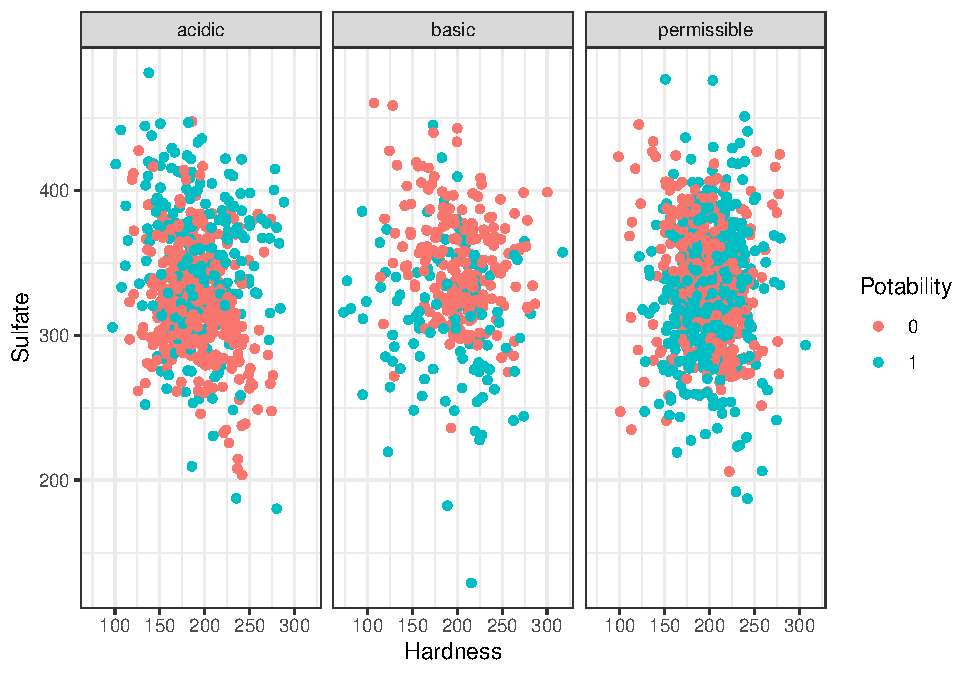
\includegraphics{_main_files/figure-latex/unnamed-chunk-64-1.pdf}

\subsection{Review with Datasaurus Dozen}\label{review-with-datasaurus-dozen}

The Datasaurus Dozen dataset is a handful of data points that complement the \texttt{dplyr} package. Aside from functions, packages can also import objects.

\begin{Shaded}
\begin{Highlighting}[]
\CommentTok{\#install.packages("datasauRus")}
\FunctionTok{library}\NormalTok{(datasauRus)}
\FunctionTok{library}\NormalTok{(tidyverse)}
\end{Highlighting}
\end{Shaded}

\begin{Shaded}
\begin{Highlighting}[]
\FunctionTok{summary}\NormalTok{(datasaurus\_dozen)}
\end{Highlighting}
\end{Shaded}

\begin{verbatim}
##    dataset                x               y           
##  Length:1846        Min.   :15.56   Min.   : 0.01512  
##  Class :character   1st Qu.:41.07   1st Qu.:22.56107  
##  Mode  :character   Median :52.59   Median :47.59445  
##                     Mean   :54.27   Mean   :47.83510  
##                     3rd Qu.:67.28   3rd Qu.:71.81078  
##                     Max.   :98.29   Max.   :99.69468
\end{verbatim}

\begin{Shaded}
\begin{Highlighting}[]
\NormalTok{datasaurus\_dozen}\SpecialCharTok{$}\NormalTok{dataset }\OtherTok{\textless{}{-}} \FunctionTok{as.factor}\NormalTok{(datasaurus\_dozen}\SpecialCharTok{$}\NormalTok{dataset)}

\FunctionTok{tail}\NormalTok{(datasaurus\_dozen)}
\end{Highlighting}
\end{Shaded}

\begin{verbatim}
## # A tibble: 6 x 3
##   dataset        x     y
##   <fct>      <dbl> <dbl>
## 1 wide_lines  34.7  19.6
## 2 wide_lines  33.7  26.1
## 3 wide_lines  75.6  37.1
## 4 wide_lines  40.6  89.1
## 5 wide_lines  39.1  96.5
## 6 wide_lines  34.6  89.6
\end{verbatim}

\begin{Shaded}
\begin{Highlighting}[]
\FunctionTok{table}\NormalTok{(datasaurus\_dozen}\SpecialCharTok{$}\NormalTok{dataset)}
\end{Highlighting}
\end{Shaded}

\begin{verbatim}
## 
##       away   bullseye     circle       dino       dots    h_lines high_lines 
##        142        142        142        142        142        142        142 
## slant_down   slant_up       star    v_lines wide_lines    x_shape 
##        142        142        142        142        142        142
\end{verbatim}

There are 13 different datasets in this one object. We will use tidyverse functions to take an overview look at the object, grouped by the datasets.

\begin{Shaded}
\begin{Highlighting}[]
\NormalTok{datasaurus\_dozen }\SpecialCharTok{\%\textgreater{}\%} 
  \FunctionTok{group\_by}\NormalTok{(dataset) }\SpecialCharTok{\%\textgreater{}\%} 
  \FunctionTok{summarize}\NormalTok{(}\AttributeTok{mean\_x =} \FunctionTok{mean}\NormalTok{(x), }
            \AttributeTok{mean\_y =} \FunctionTok{mean}\NormalTok{(y), }
            \AttributeTok{std\_dev\_x =} \FunctionTok{sd}\NormalTok{(x), }
            \AttributeTok{std\_dev\_y =} \FunctionTok{sd}\NormalTok{(y))}
\end{Highlighting}
\end{Shaded}

\begin{verbatim}
## # A tibble: 13 x 5
##    dataset    mean_x mean_y std_dev_x std_dev_y
##    <fct>       <dbl>  <dbl>     <dbl>     <dbl>
##  1 away         54.3   47.8      16.8      26.9
##  2 bullseye     54.3   47.8      16.8      26.9
##  3 circle       54.3   47.8      16.8      26.9
##  4 dino         54.3   47.8      16.8      26.9
##  5 dots         54.3   47.8      16.8      26.9
##  6 h_lines      54.3   47.8      16.8      26.9
##  7 high_lines   54.3   47.8      16.8      26.9
##  8 slant_down   54.3   47.8      16.8      26.9
##  9 slant_up     54.3   47.8      16.8      26.9
## 10 star         54.3   47.8      16.8      26.9
## 11 v_lines      54.3   47.8      16.8      26.9
## 12 wide_lines   54.3   47.8      16.8      26.9
## 13 x_shape      54.3   47.8      16.8      26.9
\end{verbatim}

All of the datasets have roughly the same mean and standard deviation along both the x and y axis.

Let's take a look the data graphically. We will use \texttt{filter} to extract the rows belonging to one dataset and then pipe that directly into a ggplot. Both dplyr and ggplot are developed within ``the Tidyverse'' and can use pipes, but you may not be able to pipe in base R functions or functions from different packages.

\begin{Shaded}
\begin{Highlighting}[]
\NormalTok{datasaurus\_dozen }\SpecialCharTok{\%\textgreater{}\%} 
  \FunctionTok{filter}\NormalTok{(dataset }\SpecialCharTok{==} \StringTok{"star"}\NormalTok{) }\SpecialCharTok{\%\textgreater{}\%} 
  \FunctionTok{ggplot}\NormalTok{(}\FunctionTok{aes}\NormalTok{(}\AttributeTok{x=}\NormalTok{x, }\AttributeTok{y=}\NormalTok{y)) }\SpecialCharTok{+} \CommentTok{\# PLUS SIGN, NOT PIPE FOR THIS ONE}
  \FunctionTok{geom\_point}\NormalTok{()}
\end{Highlighting}
\end{Shaded}

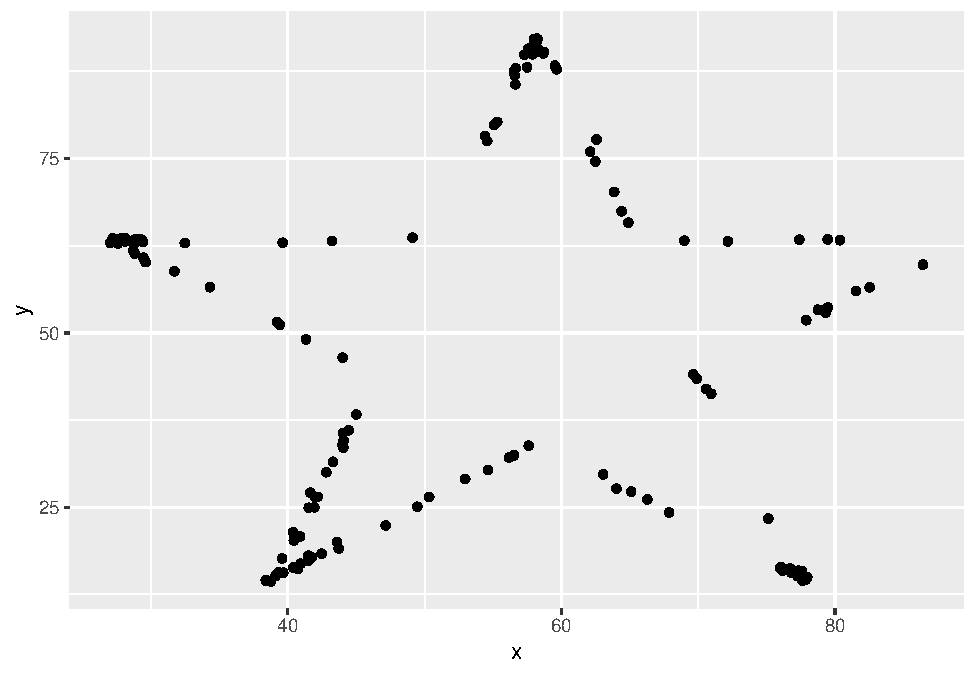
\includegraphics{_main_files/figure-latex/unnamed-chunk-68-1.pdf}

Tidyverse's data wranging packages use the pipe \texttt{\%\textgreater{}\%} to move the previous output to the next line, where as ggplot uses the plus sign \texttt{+}

Try editing the code above to display different datasets. Notice how different groups of data points can all give similar statistical summaries - so it's always a good choice to visualize your data rather than relying on just numbers.

If we wanted to take a look at all of the datasets at once, we can also use the \texttt{facet\_wrap()} function.

\begin{Shaded}
\begin{Highlighting}[]
\NormalTok{datasaurus\_dozen }\SpecialCharTok{\%\textgreater{}\%} 
  \CommentTok{\#filter(dataset == "star") \%\textgreater{}\%  REMOVE THIS ROW}
  \FunctionTok{ggplot}\NormalTok{(}\FunctionTok{aes}\NormalTok{(}\AttributeTok{x=}\NormalTok{x, }\AttributeTok{y=}\NormalTok{y)) }\SpecialCharTok{+} 
  \FunctionTok{geom\_point}\NormalTok{() }\SpecialCharTok{+} 
  \FunctionTok{facet\_wrap}\NormalTok{(}\SpecialCharTok{\textasciitilde{}}\NormalTok{dataset)}\SpecialCharTok{+} \FunctionTok{theme\_void}\NormalTok{() }\CommentTok{\# ADD THIS LINE}
\end{Highlighting}
\end{Shaded}

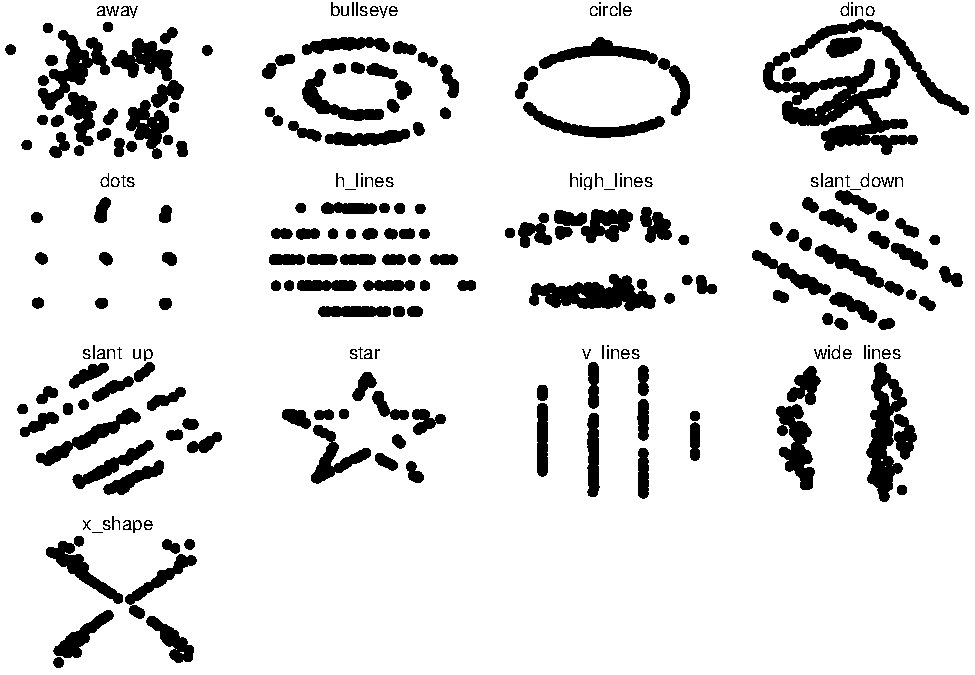
\includegraphics{_main_files/figure-latex/unnamed-chunk-69-1.pdf}

\begin{Shaded}
\begin{Highlighting}[]
\FunctionTok{head}\NormalTok{(datasaurus\_dozen)}
\end{Highlighting}
\end{Shaded}

\begin{verbatim}
## # A tibble: 6 x 3
##   dataset     x     y
##   <fct>   <dbl> <dbl>
## 1 dino     55.4  97.2
## 2 dino     51.5  96.0
## 3 dino     46.2  94.5
## 4 dino     42.8  91.4
## 5 dino     40.8  88.3
## 6 dino     38.7  84.9
\end{verbatim}

\subsection{Generalizable Code}\label{generalizable-code}

A major strength of programming is the ability to automate repetitive tasks. As a general rule of thumb, if you need to do a task more than three times (ex. analyzing multiple PCR plates or integrating clinical data from multiple days), it is worth it to invest time to write generalizable code or a custom function.

Now that we're getting comfortable writing code, we will spend some time revisiting code that we wrote to make them generalizable and even better! Generalizable means that the code is flexible and can be applied to multiple similar objects. For example, if we're running a clinical study and we have patient demographic data from multiple sites, we want to check that the mean patient demographic is comparable between sites by creating similar plots of each hospital site to compare. If we write code for one location and then copy and paste it into another code chunk to apply to the next location, the code may require some modification before it works.

Generalizable code begins at data collection. Depending on your workflow, you may or may not be able to influence this stage of the analysis. If possible, it is best practice to keep the column names and entries for categorical variables consistent. For example, when recording the age of patients, ``6'', ``6'', ``six'', and ``Six'' are all considered different levels of the factor so you will need to either make sure data collection is consistent or check and correct these inconsistencies in your code. Get into a habit of checking your work. Whether it is code you've written yourself, code you you've been sent by a collaborator, or published data from a biobank - never assume the data is as you predicted.

\subsection{Generalizable Plots}\label{generalizable-plots}

Remember when we edited our code to test out multiple datasets in the datasaurus dozen object? Perhaps you copy and pasted the code several time and changed the column name? This is not optimal because if you need to change the code in one instance (for example changing the x-axis label), you'll need to revisit ever instance that you copy and pasted to code to. This approach leads you vulnerable to errors when copy and pasting.

One way to make your code robust is to bring all the factors that need editing to the start of the data. This may seem cumbersome for such a simple example where we are only changing the dataset name, but we'll return to this concept later with more complicated examples.

Let's grab the code we used to make one plot earlier and modify it to be more generalizable

\begin{Shaded}
\begin{Highlighting}[]
\FunctionTok{levels}\NormalTok{(datasaurus\_dozen}\SpecialCharTok{$}\NormalTok{dataset)}
\end{Highlighting}
\end{Shaded}

\begin{verbatim}
##  [1] "away"       "bullseye"   "circle"     "dino"       "dots"      
##  [6] "h_lines"    "high_lines" "slant_down" "slant_up"   "star"      
## [11] "v_lines"    "wide_lines" "x_shape"
\end{verbatim}

\begin{Shaded}
\begin{Highlighting}[]
\NormalTok{dataset\_name }\OtherTok{\textless{}{-}} \StringTok{"dino"} \CommentTok{\# ADD THIS LINE}

\NormalTok{datasaurus\_dozen }\SpecialCharTok{\%\textgreater{}\%} 
  \FunctionTok{filter}\NormalTok{(dataset }\SpecialCharTok{==}\NormalTok{ dataset\_name) }\SpecialCharTok{\%\textgreater{}\%} \CommentTok{\# Remove comment \# CHANGE VARIABLE NAME}
  \FunctionTok{ggplot}\NormalTok{(}\FunctionTok{aes}\NormalTok{(}\AttributeTok{x=}\NormalTok{x, }\AttributeTok{y=}\NormalTok{y)) }\SpecialCharTok{+} 
  \FunctionTok{geom\_point}\NormalTok{() }\CommentTok{\# REMOVE THE + at the end of the line}
\end{Highlighting}
\end{Shaded}

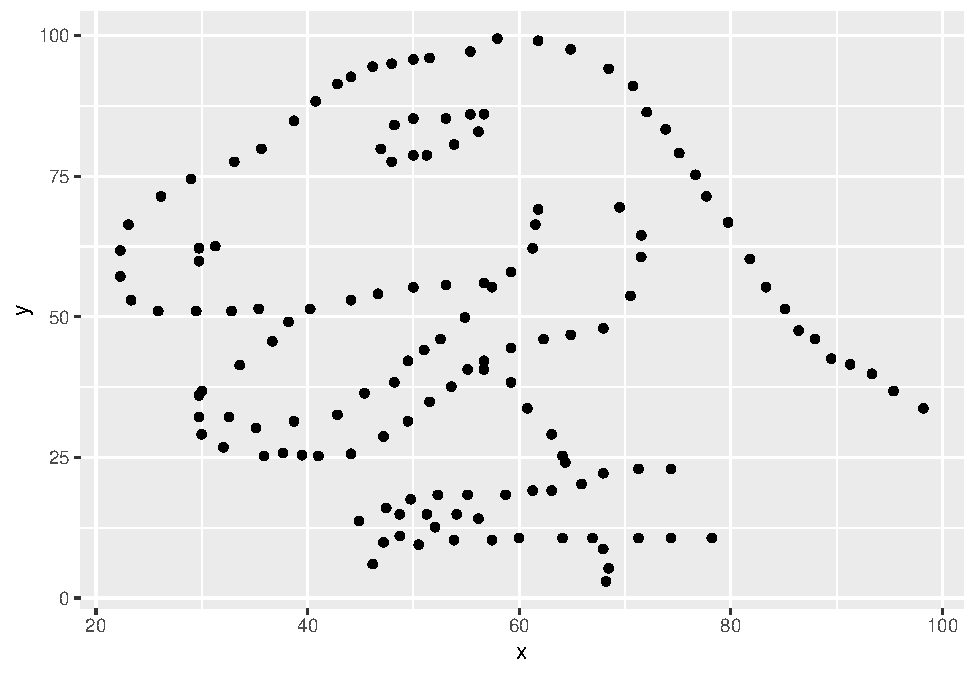
\includegraphics{_main_files/figure-latex/unnamed-chunk-71-1.pdf}

Once we have converted our code to a generalized format, we can convert it into a more versatile custom function!

Curly brackets are used for inputting multiple lines of code. It is generally attached to the function that proceeds it.

\begin{Shaded}
\begin{Highlighting}[]
\CommentTok{\# dataset\_name \textless{}{-} "dino" \# ADD THIS LINE}

\NormalTok{dino\_plot }\OtherTok{\textless{}{-}} \ControlFlowTok{function}\NormalTok{(data\_name) \{}
\NormalTok{  datasaurus\_dozen }\SpecialCharTok{\%\textgreater{}\%} 
    \FunctionTok{filter}\NormalTok{(dataset }\SpecialCharTok{==}\NormalTok{ data\_name) }\SpecialCharTok{\%\textgreater{}\%} \CommentTok{\# CHANGE ARGUMENT NAME}
    
    \FunctionTok{ggplot}\NormalTok{(}\FunctionTok{aes}\NormalTok{(}\AttributeTok{x=}\NormalTok{x, }\AttributeTok{y=}\NormalTok{y)) }\SpecialCharTok{+} 
    \FunctionTok{geom\_point}\NormalTok{() }\SpecialCharTok{+}
    \FunctionTok{theme\_bw}\NormalTok{()}
\NormalTok{\}}

\FunctionTok{dino\_plot}\NormalTok{(}\StringTok{"dino"}\NormalTok{)}
\end{Highlighting}
\end{Shaded}

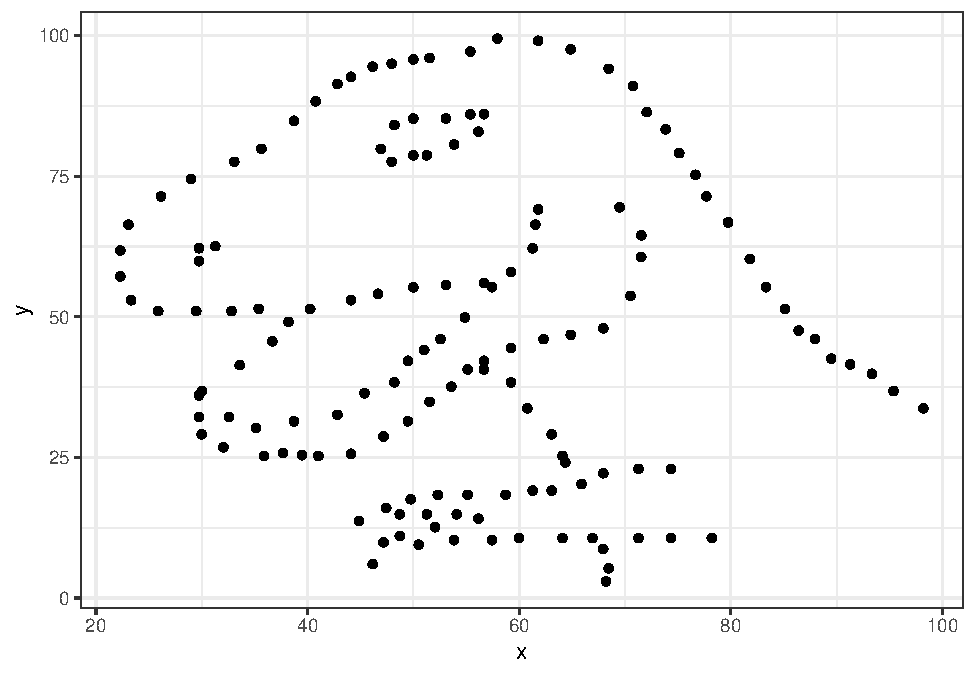
\includegraphics{_main_files/figure-latex/unnamed-chunk-72-1.pdf}

\begin{Shaded}
\begin{Highlighting}[]
\FunctionTok{dino\_plot}\NormalTok{(}\StringTok{"circle"}\NormalTok{)}
\end{Highlighting}
\end{Shaded}

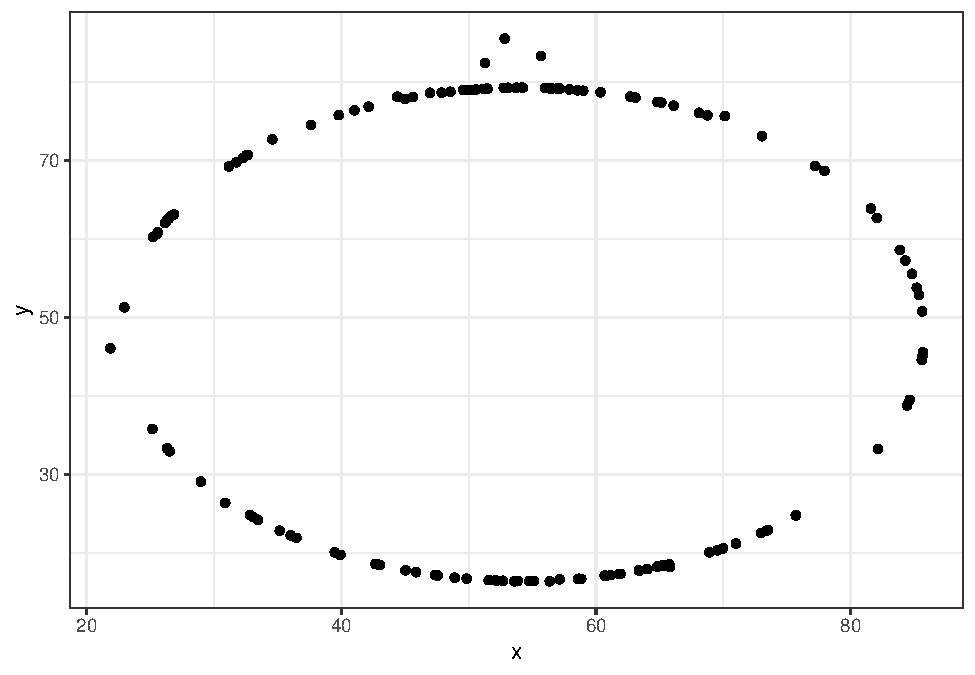
\includegraphics{_main_files/figure-latex/unnamed-chunk-72-2.pdf}

\subsection{Exercise}\label{exercise-3}

We've now encountered round brackets \texttt{()}, square brackets \texttt{{[}{]}}, and curly brackets\texttt{\{\}} - each have their own distinct functions! Take a few moments to chat with your neighbors and outline cases in which we've used each bracket and what is their role in R syntax.

round brackets ()
come after a function, function will apply to whatever is in the brackets
functionName(what is being acted on)

square brackets {[}{]}
Indexing, locations
object{[}position{]}
dataframe{[}rows, cols{]}

curly brackets \{\}
Used in function, indicate multiple lines of related code
Rmd -- indicates language in code chunk

\subsection{Dataset - Heart Stroke Prediction}\label{dataset---heart-stroke-prediction}

The dataset we will be working with for today's workshop contains clinical data collected with the aim of predicting whether a patient is likely to suffer a stroke.

The dataset can be found: \url{https://www.kaggle.com/datasets/fedesoriano/stroke-prediction-dataset}

Here is some more information about the columns in this dataset:

\begin{enumerate}
\def\labelenumi{\arabic{enumi})}
\tightlist
\item
  id: unique identifier
\item
  gender: ``Male'', ``Female'' or ``Other''
\item
  age: age of the patient
\item
  hypertension: 0 if the patient doesn't have hypertension, 1 if the patient has hypertension
\item
  heart\_disease: 0 if the patient doesn't have any heart diseases, 1 if the patient has a heart disease
\item
  ever\_married: ``No'' or ``Yes''
\item
  work\_type: ``children'', ``Govt\_jov'', ``Never\_worked'', ``Private'' or ``Self-employed''
\item
  Residence\_type: ``Rural'' or ``Urban''
\item
  avg\_glucose\_level: average glucose level in blood
\item
  bmi: body mass index
\item
  smoking\_status: ``formerly smoked'', ``never smoked'', ``smokes'' or ``Unknown''*
\item
  stroke: 1 if the patient had a stroke or 0 if not
\end{enumerate}

``Unknown'' in smoking\_status means that the information is unavailable for this patient

Let's get started!

\subsection{Exercise}\label{exercise-4}

Reading in the dataset can be an intimidating step when you're just starting out with programming. Since this is a csv file, we can use the appropriately named \texttt{read.csv()} function. In cases when you have other file types such as .txt or .tab files that are tab deliminated, there is also a \texttt{read.table()} function that is more universal (but requires more parameters to let R know how your data is stored).

Read in the \texttt{healthcare-dataset-stroke-data.csv} into an object called \texttt{heart}. Check your object using head and/or summary functions. Toggle a parameter called \texttt{stringsAsFactors} to \texttt{TRUE} in order to automatically import character values as factors rather than characters

Make sure the dataset is in the same directory or folder as this .Rmd file for ease of import

\begin{Shaded}
\begin{Highlighting}[]
\NormalTok{heart }\OtherTok{\textless{}{-}} \FunctionTok{read.csv}\NormalTok{(}\StringTok{"../INR{-}2024/datasets/healthcare{-}dataset{-}stroke{-}data.csv"}\NormalTok{, }\AttributeTok{stringsAsFactors=}\ConstantTok{TRUE}\NormalTok{)}

\FunctionTok{head}\NormalTok{(heart)}
\end{Highlighting}
\end{Shaded}

\begin{verbatim}
##      id gender age hypertension heart_disease ever_married     work_type
## 1  9046   Male  67            0             1          Yes       Private
## 2 51676 Female  61            0             0          Yes Self-employed
## 3 31112   Male  80            0             1          Yes       Private
## 4 60182 Female  49            0             0          Yes       Private
## 5  1665 Female  79            1             0          Yes Self-employed
## 6 56669   Male  81            0             0          Yes       Private
##   Residence_type avg_glucose_level  bmi  smoking_status stroke
## 1          Urban            228.69 36.6 formerly smoked      1
## 2          Rural            202.21  N/A    never smoked      1
## 3          Rural            105.92 32.5    never smoked      1
## 4          Urban            171.23 34.4          smokes      1
## 5          Rural            174.12   24    never smoked      1
## 6          Urban            186.21   29 formerly smoked      1
\end{verbatim}

\begin{Shaded}
\begin{Highlighting}[]
\FunctionTok{str}\NormalTok{(heart)}
\end{Highlighting}
\end{Shaded}

\begin{verbatim}
## 'data.frame':    5110 obs. of  12 variables:
##  $ id               : int  9046 51676 31112 60182 1665 56669 53882 10434 27419 60491 ...
##  $ gender           : Factor w/ 6 levels "female","Female",..: 4 2 4 2 2 4 4 2 2 2 ...
##  $ age              : num  67 61 80 49 79 81 74 69 59 78 ...
##  $ hypertension     : Factor w/ 4 levels "0","1","10","10+D4972": 1 1 1 1 2 1 2 1 1 1 ...
##  $ heart_disease    : int  1 0 1 0 0 0 1 0 0 0 ...
##  $ ever_married     : Factor w/ 2 levels "No","Yes": 2 2 2 2 2 2 2 1 2 2 ...
##  $ work_type        : Factor w/ 8 levels "children","Govt_job",..: 5 7 5 5 7 5 5 5 5 5 ...
##  $ Residence_type   : Factor w/ 2 levels "Rural","Urban": 2 1 1 2 1 2 1 2 1 2 ...
##  $ avg_glucose_level: num  229 202 106 171 174 ...
##  $ bmi              : Factor w/ 419 levels "10.3","11.3",..: 240 419 199 218 114 164 148 102 419 116 ...
##  $ smoking_status   : Factor w/ 4 levels "formerly smoked",..: 1 2 2 3 2 1 2 2 4 4 ...
##  $ stroke           : int  1 1 1 1 1 1 1 1 1 1 ...
\end{verbatim}

\begin{Shaded}
\begin{Highlighting}[]
\CommentTok{\# Hypertension has values that are typos, need to be removed }
\FunctionTok{table}\NormalTok{(heart}\SpecialCharTok{$}\NormalTok{hypertension)}
\end{Highlighting}
\end{Shaded}

\begin{verbatim}
## 
##        0        1       10 10+D4972 
##     4612      493        4        1
\end{verbatim}

\begin{Shaded}
\begin{Highlighting}[]
\CommentTok{\# Stroke and heart.disease need to be categorical }
\FunctionTok{summary}\NormalTok{(heart}\SpecialCharTok{$}\NormalTok{stroke)}
\end{Highlighting}
\end{Shaded}

\begin{verbatim}
##    Min. 1st Qu.  Median    Mean 3rd Qu.    Max. 
## 0.00000 0.00000 0.00000 0.04873 0.00000 1.00000
\end{verbatim}

\begin{Shaded}
\begin{Highlighting}[]
\CommentTok{\# Gender has some variability }
\FunctionTok{table}\NormalTok{(heart}\SpecialCharTok{$}\NormalTok{gender)}
\end{Highlighting}
\end{Shaded}

\begin{verbatim}
## 
## female Female   male   Male   meal  Other 
##      7   2987      6   2108      1      1
\end{verbatim}

\begin{Shaded}
\begin{Highlighting}[]
\CommentTok{\# Abnormal BMI value AND convert from factor to numeric }
\FunctionTok{summary}\NormalTok{(heart}\SpecialCharTok{$}\NormalTok{bmi)}
\end{Highlighting}
\end{Shaded}

\begin{verbatim}
##     N/A    28.7    28.4    26.1    26.7    27.6    27.7    23.4    27.3      27 
##     201      41      38      37      37      37      37      36      36      35 
##    25.1    26.4    26.9    25.5    23.5    24.8    28.9    22.2    26.5    28.3 
##      34      34      34      33      31      31      31      30      30      30 
##    29.4    30.3    31.4    24.2    26.6    27.5    28.1    29.1      24    24.1 
##      30      30      30      29      29      29      29      29      28      28 
##    25.3    27.1    27.9      28    32.3    21.5      23    24.9      25    26.2 
##      28      28      28      28      28      27      27      27      27      27 
##    28.5    28.6    29.7      30    30.9    31.5    24.3    24.5    25.4    28.8 
##      27      27      27      27      27      27      26      26      26      26 
##      29    29.2    29.5    29.6    29.9    30.1    31.1    20.1    22.7    22.8 
##      26      26      26      26      26      26      26      25      25      25 
##      26    28.2    32.8    33.1    23.6    23.9    25.8    25.9    27.2    30.5 
##      25      25      25      25      24      24      24      24      24      24 
##    31.8    32.1    35.8    20.4    24.4    26.3    27.8    29.8    30.7    33.5 
##      24      24      24      23      23      23      23      23      23      23 
##    21.4    22.1    22.4    23.8    24.6    24.7    27.4    29.3      31    31.9 
##      22      22      22      22      22      22      22      22      22      22 
##    19.5    21.3    23.1    25.6    26.8    30.8    31.3    31.6      32 (Other) 
##      21      21      21      21      21      21      21      21      21    2282
\end{verbatim}

\begin{Shaded}
\begin{Highlighting}[]
\CommentTok{\# Age, very low value of 0.08}
\FunctionTok{str}\NormalTok{(heart) }
\end{Highlighting}
\end{Shaded}

\begin{verbatim}
## 'data.frame':    5110 obs. of  12 variables:
##  $ id               : int  9046 51676 31112 60182 1665 56669 53882 10434 27419 60491 ...
##  $ gender           : Factor w/ 6 levels "female","Female",..: 4 2 4 2 2 4 4 2 2 2 ...
##  $ age              : num  67 61 80 49 79 81 74 69 59 78 ...
##  $ hypertension     : Factor w/ 4 levels "0","1","10","10+D4972": 1 1 1 1 2 1 2 1 1 1 ...
##  $ heart_disease    : int  1 0 1 0 0 0 1 0 0 0 ...
##  $ ever_married     : Factor w/ 2 levels "No","Yes": 2 2 2 2 2 2 2 1 2 2 ...
##  $ work_type        : Factor w/ 8 levels "children","Govt_job",..: 5 7 5 5 7 5 5 5 5 5 ...
##  $ Residence_type   : Factor w/ 2 levels "Rural","Urban": 2 1 1 2 1 2 1 2 1 2 ...
##  $ avg_glucose_level: num  229 202 106 171 174 ...
##  $ bmi              : Factor w/ 419 levels "10.3","11.3",..: 240 419 199 218 114 164 148 102 419 116 ...
##  $ smoking_status   : Factor w/ 4 levels "formerly smoked",..: 1 2 2 3 2 1 2 2 4 4 ...
##  $ stroke           : int  1 1 1 1 1 1 1 1 1 1 ...
\end{verbatim}

Before we dive into this dataset, we get a very limited indication that the object is read in correctly by checking the Environment panel - you'll notice the new \texttt{heart} appears under Data and it lets us know that there are 5110 observations (number of patients) and 12 variables (number of clinical features with entries). You can also double click the name of the object here to open up a view of the whole dataset - caution that this can cause your machine to stall if the dataset is exceptionally large and/or your machine is running on minimal memory.

\subsection{Exercise}\label{exercise-5}

Explore the dataset! Take a look at the columns and identify some potential issues with this dataset that either warrant further investigation or correction.

There is no universally right or wrong way to do this. Perhaps the only truly incorrect way of doing this is going through the dataset which is thousands of observations line by line.

\subsection{Factors}\label{factors}

The \texttt{stringsAsFactors} parameter takes care of the character values but we still have some integer values that should be interpreted as factors.

When deciding on whether a number is a factor or should be kept numeric, consider if decimals/numbers-in-between make sense. The first two entries for \texttt{avg\_glucose\_level} are 229 and 202 - a glucose level in between would be reasonable. In contrast, the first to entries for \texttt{heart\_disease} are 1 and 0 - as these are coding for having or not having the disorder, an entry of 1.2 does not make sense.

Recall from the introduction to the dataset from above:
4) hypertension: 0 if the patient doesn't have hypertension, 1 if the patient has hypertension
5) heart\_disease: 0 if the patient doesn't have any heart diseases, 1 if the patient has a heart disease
12) stroke: 1 if the patient had a stroke or 0 if not

\begin{Shaded}
\begin{Highlighting}[]
\NormalTok{heart}\SpecialCharTok{$}\NormalTok{hypertension }\OtherTok{\textless{}{-}} \FunctionTok{as.factor}\NormalTok{(heart}\SpecialCharTok{$}\NormalTok{hypertension)}
\NormalTok{heart}\SpecialCharTok{$}\NormalTok{heart\_disease }\OtherTok{\textless{}{-}} \FunctionTok{as.factor}\NormalTok{(heart}\SpecialCharTok{$}\NormalTok{heart\_disease)}
\NormalTok{heart}\SpecialCharTok{$}\NormalTok{stroke }\OtherTok{\textless{}{-}} \FunctionTok{as.factor}\NormalTok{(heart}\SpecialCharTok{$}\NormalTok{stroke)}

\FunctionTok{summary}\NormalTok{(heart)}
\end{Highlighting}
\end{Shaded}

\begin{verbatim}
##        id           gender          age          hypertension  heart_disease
##  Min.   :   67   female:   7   Min.   : 0.08   0       :4612   0:4834       
##  1st Qu.:17741   Female:2987   1st Qu.:25.00   1       : 493   1: 276       
##  Median :36932   male  :   6   Median :45.00   10      :   4                
##  Mean   :36518   Male  :2108   Mean   :43.23   10+D4972:   1                
##  3rd Qu.:54682   meal  :   1   3rd Qu.:61.00                                
##  Max.   :72940   Other :   1   Max.   :82.00                                
##                                                                             
##  ever_married         work_type    Residence_type avg_glucose_level
##  No :1757     Private      :2921   Rural:2514     Min.   : 55.12   
##  Yes:3353     Self-employed: 818   Urban:2596     1st Qu.: 77.25   
##               children     : 687                  Median : 91.89   
##               Govt_job     : 656                  Mean   :106.15   
##               Never_worked :  22                  3rd Qu.:114.09   
##               Private      :   4                  Max.   :271.74   
##               (Other)      :   2                                   
##       bmi               smoking_status stroke  
##  N/A    : 201   formerly smoked: 885   0:4861  
##  28.7   :  41   never smoked   :1892   1: 249  
##  28.4   :  38   smokes         : 789           
##  26.1   :  37   Unknown        :1544           
##  26.7   :  37                                  
##  27.6   :  37                                  
##  (Other):4719
\end{verbatim}

\subsection{Incomplete Data}\label{incomplete-data}

Firstly, we have to make a decision on how to handle missing values. We can either accept that some of the columns are incomplete or eliminate rows that do not have full data. Let's evaluate which columns this affects

If you ever encounter missing data when you are entering data, use \texttt{NA}.

\begin{Shaded}
\begin{Highlighting}[]
\FunctionTok{ggplot}\NormalTok{(heart, }\FunctionTok{aes}\NormalTok{(}\AttributeTok{x =}\NormalTok{ smoking\_status, }\AttributeTok{fill =}\NormalTok{ hypertension)) }\SpecialCharTok{+} 
  \FunctionTok{geom\_bar}\NormalTok{()}
\end{Highlighting}
\end{Shaded}

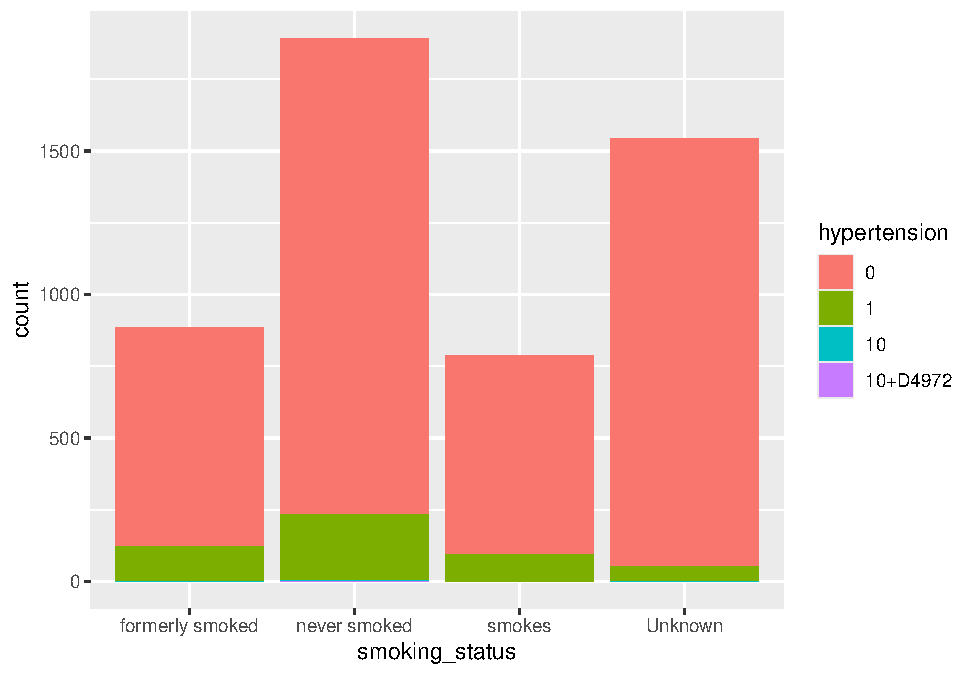
\includegraphics{_main_files/figure-latex/unnamed-chunk-76-1.pdf}

\begin{Shaded}
\begin{Highlighting}[]
\FunctionTok{prop.table}\NormalTok{(}\FunctionTok{table}\NormalTok{(heart}\SpecialCharTok{$}\NormalTok{smoking\_status, heart}\SpecialCharTok{$}\NormalTok{hypertension))}
\end{Highlighting}
\end{Shaded}

\begin{verbatim}
##                  
##                              0            1           10     10+D4972
##   formerly smoked 0.1497064579 0.0232876712 0.0001956947 0.0000000000
##   never smoked    0.3248532290 0.0448140900 0.0003913894 0.0001956947
##   smokes          0.1360078278 0.0183953033 0.0000000000 0.0000000000
##   Unknown         0.2919765166 0.0099804305 0.0001956947 0.0000000000
\end{verbatim}

Let's use tidyverse to remove the rows in the \texttt{smoking\_status} column with a value of \texttt{Unknown}.

\begin{Shaded}
\begin{Highlighting}[]
\FunctionTok{dim}\NormalTok{(heart) }\CommentTok{\# original 5110 rows }
\end{Highlighting}
\end{Shaded}

\begin{verbatim}
## [1] 5110   12
\end{verbatim}

\begin{Shaded}
\begin{Highlighting}[]
\FunctionTok{table}\NormalTok{(heart}\SpecialCharTok{$}\NormalTok{smoking\_status) }\CommentTok{\#1544 unknowns}
\end{Highlighting}
\end{Shaded}

\begin{verbatim}
## 
## formerly smoked    never smoked          smokes         Unknown 
##             885            1892             789            1544
\end{verbatim}

\begin{Shaded}
\begin{Highlighting}[]
\FunctionTok{dim}\NormalTok{(}\FunctionTok{filter}\NormalTok{(heart, }\SpecialCharTok{!}\NormalTok{(smoking\_status }\SpecialCharTok{==} \StringTok{"Unknown"}\NormalTok{)))}
\end{Highlighting}
\end{Shaded}

\begin{verbatim}
## [1] 3566   12
\end{verbatim}

\begin{Shaded}
\begin{Highlighting}[]
\NormalTok{heart }\OtherTok{\textless{}{-}} \FunctionTok{filter}\NormalTok{(heart, }\SpecialCharTok{!}\NormalTok{(smoking\_status }\SpecialCharTok{==} \StringTok{"Unknown"}\NormalTok{))}
\FunctionTok{summary}\NormalTok{(heart}\SpecialCharTok{$}\NormalTok{smoking\_status)}
\end{Highlighting}
\end{Shaded}

\begin{verbatim}
## formerly smoked    never smoked          smokes         Unknown 
##             885            1892             789               0
\end{verbatim}

After double checking, we can see that the smoking status has an empty level, we'll clean this up before moving on

\begin{Shaded}
\begin{Highlighting}[]
\NormalTok{heart}\SpecialCharTok{$}\NormalTok{smoking\_status }\OtherTok{\textless{}{-}} \FunctionTok{droplevels}\NormalTok{(heart}\SpecialCharTok{$}\NormalTok{smoking\_status)}

\FunctionTok{summary}\NormalTok{(heart}\SpecialCharTok{$}\NormalTok{smoking\_status)}
\end{Highlighting}
\end{Shaded}

\begin{verbatim}
## formerly smoked    never smoked          smokes 
##             885            1892             789
\end{verbatim}

\begin{Shaded}
\begin{Highlighting}[]
\NormalTok{heart\_checkpoint }\OtherTok{\textless{}{-}}\NormalTok{ heart}
\end{Highlighting}
\end{Shaded}

Great! Now let's tackle the typos in the gender column.

\begin{Shaded}
\begin{Highlighting}[]
\FunctionTok{table}\NormalTok{(heart}\SpecialCharTok{$}\NormalTok{gender)}
\end{Highlighting}
\end{Shaded}

\begin{verbatim}
## 
## female Female   male   Male   meal  Other 
##      5   2153      5   1402      0      1
\end{verbatim}

We need to fix the typos that happened during data entry and the single observation of \texttt{Other} will not be enough data for us to draw any statistical conclusion so we'll remove this row while we're at it.

We can use \texttt{str\_replace\_all()} as a search and replace tool

\begin{Shaded}
\begin{Highlighting}[]
\FunctionTok{table}\NormalTok{(}\FunctionTok{str\_replace\_all}\NormalTok{(heart}\SpecialCharTok{$}\NormalTok{gender, }\StringTok{"female"}\NormalTok{, }\StringTok{"Female"}\NormalTok{))}
\end{Highlighting}
\end{Shaded}

\begin{verbatim}
## 
## Female   male   Male  Other 
##   2158      5   1402      1
\end{verbatim}

\begin{Shaded}
\begin{Highlighting}[]
\CommentTok{\# str\_replace\_all(data, what we\textquotesingle{}re search, what to replace with)}
\end{Highlighting}
\end{Shaded}

Remember that this only displays the output, it does not replace the columns in the dataset.

Before we apply it globally, we can set up a quick double check to make sure that the right values are changed.

\begin{Shaded}
\begin{Highlighting}[]
\CommentTok{\# document which rows have the error "female" }
\NormalTok{wrong\_entry }\OtherTok{\textless{}{-}} \FunctionTok{which}\NormalTok{(heart}\SpecialCharTok{$}\NormalTok{gender }\SpecialCharTok{==} \StringTok{"female"}\NormalTok{)}
\NormalTok{wrong\_entry}
\end{Highlighting}
\end{Shaded}

\begin{verbatim}
## [1]  127  271  941 1930 3021
\end{verbatim}

\begin{Shaded}
\begin{Highlighting}[]
\NormalTok{heart}\SpecialCharTok{$}\NormalTok{gender[wrong\_entry]}
\end{Highlighting}
\end{Shaded}

\begin{verbatim}
## [1] female female female female female
## Levels: female Female male Male meal Other
\end{verbatim}

\begin{Shaded}
\begin{Highlighting}[]
\CommentTok{\# apply the search and replace}
\NormalTok{heart}\SpecialCharTok{$}\NormalTok{gender }\OtherTok{\textless{}{-}} \FunctionTok{str\_replace\_all}\NormalTok{(heart}\SpecialCharTok{$}\NormalTok{gender, }\FunctionTok{c}\NormalTok{(}\StringTok{"female"} \OtherTok{=} \StringTok{"Female"}\NormalTok{, }
                                                \StringTok{"male"} \OtherTok{=} \StringTok{"Male"}\NormalTok{, }
                                                \StringTok{"meal"} \OtherTok{=} \StringTok{"Male"}\NormalTok{))}

\NormalTok{heart}\SpecialCharTok{$}\NormalTok{gender[wrong\_entry]}
\end{Highlighting}
\end{Shaded}

\begin{verbatim}
## [1] "FeMale" "FeMale" "FeMale" "FeMale" "FeMale"
\end{verbatim}

\begin{Shaded}
\begin{Highlighting}[]
\FunctionTok{table}\NormalTok{(heart}\SpecialCharTok{$}\NormalTok{gender)}
\end{Highlighting}
\end{Shaded}

\begin{verbatim}
## 
## FeMale   Male  Other 
##   2158   1407      1
\end{verbatim}

There's an issue with the ``male'' search grabbing from the ``female'' word!! Good thing we made a checkpoint earlier. Let's bring this back to our main heart object - it's a good habit to make some objects to checkpoint your work. In case you have not had this set up, you can always back track in your code and re-read in the object and re-run some earlier code to catch up.

\begin{Shaded}
\begin{Highlighting}[]
\NormalTok{heart }\OtherTok{\textless{}{-}}\NormalTok{ heart\_checkpoint }

\FunctionTok{table}\NormalTok{(heart}\SpecialCharTok{$}\NormalTok{gender)}
\end{Highlighting}
\end{Shaded}

\begin{verbatim}
## 
## female Female   male   Male   meal  Other 
##      5   2153      5   1402      0      1
\end{verbatim}

Let's try this again:

\begin{Shaded}
\begin{Highlighting}[]
\CommentTok{\# From previous code }

\CommentTok{\# add \^{} (carrot) to the start of the search term to make sure it\textquotesingle{}s only found at the start of the word}
\NormalTok{heart}\SpecialCharTok{$}\NormalTok{gender }\OtherTok{\textless{}{-}} \FunctionTok{str\_replace\_all}\NormalTok{(heart}\SpecialCharTok{$}\NormalTok{gender, }\FunctionTok{c}\NormalTok{(}\StringTok{"\^{}female"} \OtherTok{=} \StringTok{"Female"}\NormalTok{, }
                                                \StringTok{"\^{}male"} \OtherTok{=} \StringTok{"Male"}\NormalTok{, }
                                                \StringTok{"\^{}meal"} \OtherTok{=} \StringTok{"Male"}\NormalTok{))}

\NormalTok{heart}\SpecialCharTok{$}\NormalTok{gender[wrong\_entry]}
\end{Highlighting}
\end{Shaded}

\begin{verbatim}
## [1] "Female" "Female" "Female" "Female" "Female"
\end{verbatim}

\begin{Shaded}
\begin{Highlighting}[]
\FunctionTok{table}\NormalTok{(heart}\SpecialCharTok{$}\NormalTok{gender)}
\end{Highlighting}
\end{Shaded}

\begin{verbatim}
## 
## Female   Male  Other 
##   2158   1407      1
\end{verbatim}

The \texttt{\^{}} is a special character that indicates the start of a word.

Lastly, we'll the one \texttt{Other} entry

\begin{Shaded}
\begin{Highlighting}[]
\NormalTok{heart }\OtherTok{\textless{}{-}}\NormalTok{ heart[}\SpecialCharTok{!}\NormalTok{heart}\SpecialCharTok{$}\NormalTok{gender }\SpecialCharTok{==} \StringTok{"Other"}\NormalTok{, ] }\CommentTok{\# object[rows, col]}
\FunctionTok{table}\NormalTok{(heart}\SpecialCharTok{$}\NormalTok{gender)}
\end{Highlighting}
\end{Shaded}

\begin{verbatim}
## 
## Female   Male 
##   2158   1407
\end{verbatim}

Overall, the data is looking much cleaner than when we started!

\subsection{Exercise}\label{exercise-6}

Investigate the \texttt{work\_type} column and correct the data entry problems! Also, remove any ``N/A'' entries under \texttt{bmi}

\begin{Shaded}
\begin{Highlighting}[]
\FunctionTok{table}\NormalTok{(heart}\SpecialCharTok{$}\NormalTok{work\_type)}
\end{Highlighting}
\end{Shaded}

\begin{verbatim}
## 
##       children       Govt_job      Govt_job    Never_worked        Private 
##             69            534              1             14           2281 
##       Private   Self-employed Self-employed  
##              3            662              1
\end{verbatim}

\begin{Shaded}
\begin{Highlighting}[]
\FunctionTok{levels}\NormalTok{(heart}\SpecialCharTok{$}\NormalTok{work\_type)}
\end{Highlighting}
\end{Shaded}

\begin{verbatim}
## [1] "children"       "Govt_job"       "Govt_job "      "Never_worked"  
## [5] "Private"        "Private "       "Self-employed"  "Self-employed "
\end{verbatim}

\begin{Shaded}
\begin{Highlighting}[]
\NormalTok{heart}\SpecialCharTok{$}\NormalTok{work\_type }\OtherTok{\textless{}{-}} \FunctionTok{str\_replace\_all}\NormalTok{(heart}\SpecialCharTok{$}\NormalTok{work\_type, }\FunctionTok{c}\NormalTok{(}\StringTok{"Govt\_job "} \OtherTok{=} \StringTok{"Govt\_job"}\NormalTok{, }
                                                      \StringTok{"Private "} \OtherTok{=} \StringTok{"Private"}\NormalTok{, }
                                                      \StringTok{"Self{-}employed "} \OtherTok{=} \StringTok{"Self{-}employed"}\NormalTok{))}

\FunctionTok{class}\NormalTok{(heart}\SpecialCharTok{$}\NormalTok{work\_type)}
\end{Highlighting}
\end{Shaded}

\begin{verbatim}
## [1] "character"
\end{verbatim}

\begin{Shaded}
\begin{Highlighting}[]
\NormalTok{heart}\SpecialCharTok{$}\NormalTok{work\_type }\OtherTok{\textless{}{-}} \FunctionTok{as.factor}\NormalTok{(heart}\SpecialCharTok{$}\NormalTok{work\_type)}
\end{Highlighting}
\end{Shaded}

\begin{Shaded}
\begin{Highlighting}[]
\FunctionTok{summary}\NormalTok{(heart}\SpecialCharTok{$}\NormalTok{bmi)}
\end{Highlighting}
\end{Shaded}

\begin{verbatim}
##     N/A    28.4    28.7      27    27.6    25.5    27.3    26.1    26.7    26.9 
##     140      32      32      30      30      28      28      26      26      26 
##    32.3    25.1    25.3    26.4    26.5    27.7    28.3    28.9      29    29.6 
##      26      25      25      25      25      25      25      24      24      24 
##    30.3    30.9    31.4    23.4      28    28.1    28.6    29.4    23.5    26.6 
##      24      24      24      23      23      23      23      23      22      22 
##    27.1    27.5    28.2    28.5    29.5    31.1    22.2    24.5      25    26.2 
##      22      22      22      22      22      22      21      21      21      21 
##    27.9    29.2    29.9      30    30.5    30.7    31.5    32.1      24    24.1 
##      21      21      21      21      21      21      21      21      20      20 
##    24.2    24.3    24.8      26    27.2    30.1    33.1    35.8    24.9    25.4 
##      20      20      20      20      20      20      20      20      19      19 
##    28.8    29.7    31.3    32.8    24.4    26.3    27.8    33.7    21.5    22.8 
##      19      19      19      19      18      18      18      18      17      17 
##    23.1    23.8    27.4    29.3      31    31.6    31.8    34.7    21.3    22.1 
##      17      17      17      17      17      17      17      17      16      16 
##    22.7      23    23.9    24.6    24.7    25.8    25.9    26.8    29.1    29.8 
##      16      16      16      16      16      16      16      16      16      16 
##    30.2    30.8    31.2    31.9    32.4    33.5    34.5    23.6    32.2 (Other) 
##      16      16      16      16      16      16      16      15      15    1414
\end{verbatim}

\begin{Shaded}
\begin{Highlighting}[]
\NormalTok{heart}\SpecialCharTok{$}\NormalTok{bmi }\OtherTok{\textless{}{-}} \FunctionTok{as.numeric}\NormalTok{(heart}\SpecialCharTok{$}\NormalTok{bmi)}
\FunctionTok{summary}\NormalTok{(heart}\SpecialCharTok{$}\NormalTok{bmi)}
\end{Highlighting}
\end{Shaded}

\begin{verbatim}
##    Min. 1st Qu.  Median    Mean 3rd Qu.    Max. 
##     3.0   128.0   168.0   185.6   223.0   419.0
\end{verbatim}

\subsection{Loops}\label{loops}

``For loops'' allow R to apply highly automated tasks. It will cycle through a range of inputs and ``for'' each of them, it will carry out your custom task.

Here's a very simple example to show you the structure of for loops

\begin{Shaded}
\begin{Highlighting}[]
\NormalTok{fruits }\OtherTok{\textless{}{-}} \FunctionTok{c}\NormalTok{(}\StringTok{"strawberry"}\NormalTok{, }\StringTok{"banana"}\NormalTok{, }\StringTok{"orange"}\NormalTok{)}

\ControlFlowTok{for}\NormalTok{(x }\ControlFlowTok{in}\NormalTok{ fruits) \{}
  \FunctionTok{print}\NormalTok{(x)}
\NormalTok{\}}
\end{Highlighting}
\end{Shaded}

\begin{verbatim}
## [1] "strawberry"
## [1] "banana"
## [1] "orange"
\end{verbatim}

The \texttt{for()} function accepts firstly the name of a temporary object that exists only within the curly brackets of the for loop, the \texttt{in} is a special R syntax specification, and \texttt{fruit} is the object that we are applying the for loop on.

The for loop will take each entry of the fruits object, store it in the temporary object \texttt{x}, and apply the code written written within the curly bracket before repeating with the next entry.

I recommend testing your code outside the \texttt{for()} loop before moving it into the loop to make sure it is robust and if you are applying the loop to a long vector or large dataset, consider trying it on a truncated version first as a proof of principle.

\begin{Shaded}
\begin{Highlighting}[]
\FunctionTok{levels}\NormalTok{(heart}\SpecialCharTok{$}\NormalTok{smoking\_status)}
\end{Highlighting}
\end{Shaded}

\begin{verbatim}
## [1] "formerly smoked" "never smoked"    "smokes"
\end{verbatim}

\begin{Shaded}
\begin{Highlighting}[]
\NormalTok{heart }\SpecialCharTok{\%\textgreater{}\%} 
  \FunctionTok{filter}\NormalTok{(smoking\_status }\SpecialCharTok{==} \StringTok{"never smoked"}\NormalTok{) }\SpecialCharTok{\%\textgreater{}\%} 
  \FunctionTok{ggplot}\NormalTok{(}\FunctionTok{aes}\NormalTok{(}\AttributeTok{x=}\NormalTok{avg\_glucose\_level, }\AttributeTok{y=}\NormalTok{bmi)) }\SpecialCharTok{+}
  \FunctionTok{geom\_point}\NormalTok{() }\SpecialCharTok{+} 
  \FunctionTok{ggtitle}\NormalTok{(}\StringTok{"never smoked"}\NormalTok{) }\SpecialCharTok{+}
  \FunctionTok{theme\_classic}\NormalTok{()}
\end{Highlighting}
\end{Shaded}

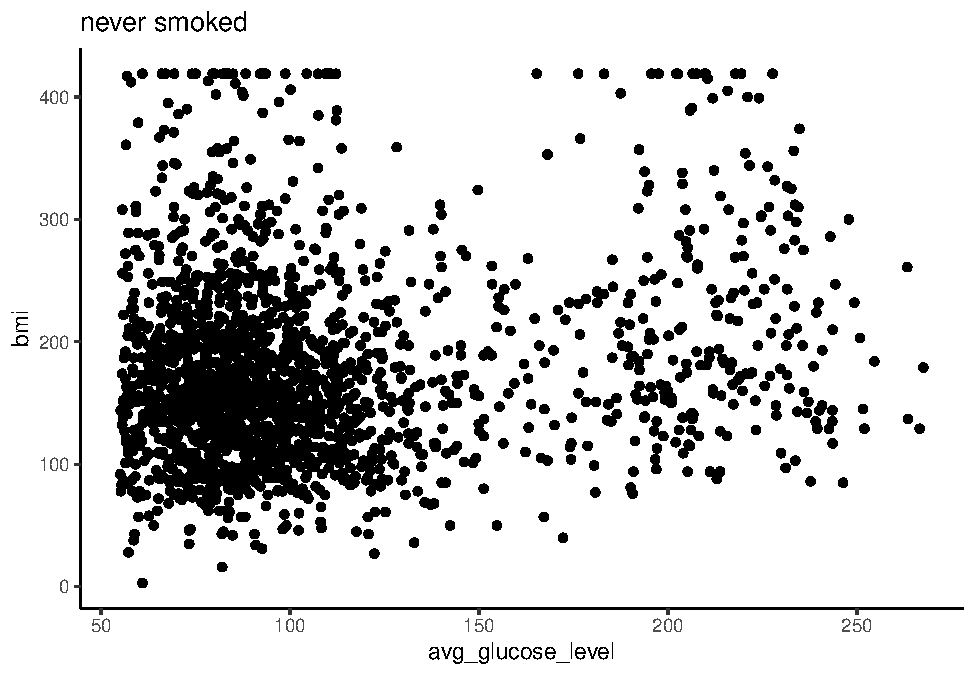
\includegraphics{_main_files/figure-latex/unnamed-chunk-88-1.pdf}

If we wanted to save a pdf of every category of \texttt{smoking\_status}, we can convert our code into a loop. When working on a larger section of code, it is helpful to sketch out the steps you need to do with \texttt{\#} comments to keep you focused.

\begin{Shaded}
\begin{Highlighting}[]
\NormalTok{smoke\_cat }\OtherTok{\textless{}{-}} \FunctionTok{levels}\NormalTok{(heart}\SpecialCharTok{$}\NormalTok{smoking\_status)}
\NormalTok{smoke\_cat}
\end{Highlighting}
\end{Shaded}

\begin{verbatim}
## [1] "formerly smoked" "never smoked"    "smokes"
\end{verbatim}

\begin{Shaded}
\begin{Highlighting}[]
\FunctionTok{getwd}\NormalTok{() }\CommentTok{\# get working directory}
\end{Highlighting}
\end{Shaded}

\begin{verbatim}
## [1] "/Users/clin/Documents/CBWGitHub/INR_2024"
\end{verbatim}

\begin{Shaded}
\begin{Highlighting}[]
\ControlFlowTok{for}\NormalTok{(cat }\ControlFlowTok{in}\NormalTok{ smoke\_cat) \{}
  
  \CommentTok{\# Specify file name}
\NormalTok{  filename\_cat }\OtherTok{\textless{}{-}} \FunctionTok{paste0}\NormalTok{(}\StringTok{"bmi\_glucose\_"}\NormalTok{, cat, }\StringTok{".png"}\NormalTok{)}
  \FunctionTok{print}\NormalTok{(filename\_cat)}
  
  \CommentTok{\# Making plot (based on code from above)}
  
\NormalTok{  plot\_cat }\OtherTok{\textless{}{-}}\NormalTok{ heart }\SpecialCharTok{\%\textgreater{}\%} \CommentTok{\# SAVE OUTPUT TO OBJECT}
  \FunctionTok{filter}\NormalTok{(smoking\_status }\SpecialCharTok{==}\NormalTok{ cat) }\SpecialCharTok{\%\textgreater{}\%} \CommentTok{\# CHANGE TO cat}
  \FunctionTok{ggplot}\NormalTok{(}\FunctionTok{aes}\NormalTok{(}\AttributeTok{x=}\NormalTok{avg\_glucose\_level, }\AttributeTok{y=}\NormalTok{bmi)) }\SpecialCharTok{+}
  \FunctionTok{geom\_point}\NormalTok{() }\SpecialCharTok{+} 
  \FunctionTok{ggtitle}\NormalTok{(cat) }\SpecialCharTok{+} \CommentTok{\# CHANGE TO cat}
  \FunctionTok{theme\_classic}\NormalTok{()}
  
  \CommentTok{\#print(plot\_cat) \# PRINT OUT PLOT}
  
  \CommentTok{\# Saving the plot to file }
  \FunctionTok{png}\NormalTok{(filename\_cat, }\AttributeTok{width =} \DecValTok{700}\NormalTok{, }\AttributeTok{height=} \DecValTok{500}\NormalTok{, }\AttributeTok{res=}\DecValTok{120}\NormalTok{) }\CommentTok{\# Start saving whatever I make now to this file }
  \FunctionTok{print}\NormalTok{(plot\_cat)}
  \FunctionTok{dev.off}\NormalTok{() }\CommentTok{\# Stop saving}
\NormalTok{\}}
\end{Highlighting}
\end{Shaded}

\begin{verbatim}
## [1] "bmi_glucose_formerly smoked.png"
\end{verbatim}

\begin{verbatim}
## [1] "bmi_glucose_never smoked.png"
\end{verbatim}

\begin{verbatim}
## [1] "bmi_glucose_smokes.png"
\end{verbatim}

\subsection{Exercise}\label{exercise-7}

Copy and paste the loop from above and modify it so that the range of values on the x and y axis are the same for all plots.

The limits of the x axis can be specified by adding a layer called \texttt{xlim(lower,\ upper)} where it takes two numbers - the lower limit followed by the upper limit. These numbers can be stored in objects or inputted directly . Similarly, there is a parallel function called \texttt{ylim()} which also takes the same two parameters

When working through the code, you can temporarily remove the code removing the axis labels by commenting out the lines with a hashtag.

Great! Now the y-axis does not change between the plots and they are directly comparable.

\subsection{Conditional for Loops}\label{conditional-for-loops}

Boolean statements can be used to write conditional statements. If we do not want the loop to be applied to every item, we can add a condition.

\begin{Shaded}
\begin{Highlighting}[]
\NormalTok{food }\OtherTok{\textless{}{-}} \StringTok{"pineapple"}

\ControlFlowTok{if}\NormalTok{(food }\SpecialCharTok{==} \StringTok{"pineapple"}\NormalTok{) \{}
  \FunctionTok{print}\NormalTok{(}\StringTok{"This indeed is a pineapple."}\NormalTok{)}
\NormalTok{\}}
\end{Highlighting}
\end{Shaded}

\begin{verbatim}
## [1] "This indeed is a pineapple."
\end{verbatim}

This will only output if the condition is met. We can also modify this statement to do something in case the condition is not met.

\begin{Shaded}
\begin{Highlighting}[]
\NormalTok{food }\OtherTok{\textless{}{-}} \StringTok{"orange"}

\ControlFlowTok{if}\NormalTok{(food }\SpecialCharTok{==} \StringTok{"pineapple"}\NormalTok{) \{}
  \FunctionTok{print}\NormalTok{(}\StringTok{"This indeed is a pineapple."}\NormalTok{)}
\NormalTok{\} }\ControlFlowTok{else}\NormalTok{ \{}
  \FunctionTok{print}\NormalTok{(}\StringTok{"This is NOT a pineapple."}\NormalTok{)}
\NormalTok{\}}
\end{Highlighting}
\end{Shaded}

\begin{verbatim}
## [1] "This is NOT a pineapple."
\end{verbatim}

Using \texttt{if\ else} statements will allow more customizability in our code. Let's use this to add a new column called \texttt{ever\_smoked} based on the value in the \texttt{smoking\_status} column.

\begin{Shaded}
\begin{Highlighting}[]
\FunctionTok{table}\NormalTok{(heart}\SpecialCharTok{$}\NormalTok{stroke)}
\end{Highlighting}
\end{Shaded}

\begin{verbatim}
## 
##    0    1 
## 3363  202
\end{verbatim}

\begin{Shaded}
\begin{Highlighting}[]
\NormalTok{heart}\SpecialCharTok{$}\NormalTok{stroke\_history }\OtherTok{\textless{}{-}} \ConstantTok{NA}
\FunctionTok{head}\NormalTok{(heart)}
\end{Highlighting}
\end{Shaded}

\begin{verbatim}
##      id gender age hypertension heart_disease ever_married     work_type
## 1  9046   Male  67            0             1          Yes       Private
## 2 51676 Female  61            0             0          Yes Self-employed
## 3 31112   Male  80            0             1          Yes       Private
## 4 60182 Female  49            0             0          Yes       Private
## 5  1665 Female  79            1             0          Yes Self-employed
## 6 56669   Male  81            0             0          Yes       Private
##   Residence_type avg_glucose_level bmi  smoking_status stroke stroke_history
## 1          Urban            228.69 240 formerly smoked      1             NA
## 2          Rural            202.21 419    never smoked      1             NA
## 3          Rural            105.92 199    never smoked      1             NA
## 4          Urban            171.23 218          smokes      1             NA
## 5          Rural            174.12 114    never smoked      1             NA
## 6          Urban            186.21 164 formerly smoked      1             NA
\end{verbatim}

\begin{Shaded}
\begin{Highlighting}[]
\ControlFlowTok{for}\NormalTok{(row }\ControlFlowTok{in} \DecValTok{1}\SpecialCharTok{:}\FunctionTok{nrow}\NormalTok{(heart)) \{}
  \ControlFlowTok{if}\NormalTok{(heart}\SpecialCharTok{$}\NormalTok{stroke[row] }\SpecialCharTok{==} \StringTok{"1"}\NormalTok{) \{}
\NormalTok{    heart}\SpecialCharTok{$}\NormalTok{stroke\_history[row] }\OtherTok{\textless{}{-}} \StringTok{"confirmed\_stroke"}
\NormalTok{  \} }\ControlFlowTok{else}\NormalTok{ \{ }
\NormalTok{    heart}\SpecialCharTok{$}\NormalTok{stroke\_history[row] }\OtherTok{\textless{}{-}} \StringTok{"no\_history"}
\NormalTok{    \}}
  \CommentTok{\# else \textgreater{}\textgreater{} "no\_history" }
  
\NormalTok{\}}
\FunctionTok{table}\NormalTok{(heart}\SpecialCharTok{$}\NormalTok{stroke, heart}\SpecialCharTok{$}\NormalTok{stroke\_history)}
\end{Highlighting}
\end{Shaded}

\begin{verbatim}
##    
##     confirmed_stroke no_history
##   0                0       3363
##   1              202          0
\end{verbatim}

\subsection{Exercise}\label{exercise-8}

Expected fasting blood glucose concentrations defined by the WHO are between 70 - 100 mg/dL. Create a new column called \texttt{glucose\_WHO} in which:

\begin{itemize}
\tightlist
\item
  \texttt{avg\_glucose\_levels} less than 70 are annotated as \texttt{followup}
\item
  \texttt{avg\_glucose\_levels} between 70-100 are annotated as \texttt{average}
\item
  \texttt{avg\_glucose\_levels} over 100 are annotated as \texttt{followup}
\end{itemize}

Conditions can be combined using the \texttt{\&} for \texttt{and} where as \texttt{\textbar{}} is used for \texttt{or} statements.

\begin{Shaded}
\begin{Highlighting}[]
\FunctionTok{colnames}\NormalTok{(heart) }\CommentTok{\# SHOULD BE \textquotesingle{}avg\_glucose\_level\textquotesingle{} WITHOUT THE S AT THE }\RegionMarkerTok{END}\CommentTok{ }
\end{Highlighting}
\end{Shaded}

\begin{verbatim}
##  [1] "id"                "gender"            "age"              
##  [4] "hypertension"      "heart_disease"     "ever_married"     
##  [7] "work_type"         "Residence_type"    "avg_glucose_level"
## [10] "bmi"               "smoking_status"    "stroke"           
## [13] "stroke_history"
\end{verbatim}

\begin{Shaded}
\begin{Highlighting}[]
\CommentTok{\# Sorry! }

\NormalTok{heart}\SpecialCharTok{$}\NormalTok{glucose\_WHO }\OtherTok{\textless{}{-}} \ConstantTok{NA}

\ControlFlowTok{for}\NormalTok{(row }\ControlFlowTok{in} \DecValTok{1}\SpecialCharTok{:}\FunctionTok{nrow}\NormalTok{(heart)) \{ }
  \ControlFlowTok{if}\NormalTok{(heart}\SpecialCharTok{$}\NormalTok{avg\_glucose\_level[row] }\SpecialCharTok{\textgreater{}} \DecValTok{70} \SpecialCharTok{\&}\NormalTok{ heart}\SpecialCharTok{$}\NormalTok{avg\_glucose\_level[row] }\SpecialCharTok{\textless{}} \DecValTok{100}\NormalTok{) \{}
\NormalTok{  heart}\SpecialCharTok{$}\NormalTok{glucose\_WHO[row] }\OtherTok{\textless{}{-}} \StringTok{"average"}
\NormalTok{  \} }\ControlFlowTok{else}\NormalTok{ \{ }
\NormalTok{    heart}\SpecialCharTok{$}\NormalTok{glucose\_WHO[row] }\OtherTok{\textless{}{-}} \StringTok{"followup"}\NormalTok{\}}
\NormalTok{\}}

\FunctionTok{table}\NormalTok{(heart}\SpecialCharTok{$}\NormalTok{glucose\_WHO)}
\end{Highlighting}
\end{Shaded}

\begin{verbatim}
## 
##  average followup 
##     1610     1955
\end{verbatim}

\subsection{Countinous Variables}\label{countinous-variables}

In the heart dataset, we have three continuous variables. In R, continuous variables will be \texttt{numeric} values. Continuous variable have a wide range of ordered values. For example, the \texttt{age} values have a range of 10 to 82 - any value in between is possible.

\begin{Shaded}
\begin{Highlighting}[]
\CommentTok{\#heart$bmi \textless{}{-} as.numeric(heart$bmi)}

\FunctionTok{ggplot}\NormalTok{(heart, }\FunctionTok{aes}\NormalTok{(}\AttributeTok{x=}\NormalTok{bmi)) }\SpecialCharTok{+} 
  \FunctionTok{geom\_histogram}\NormalTok{()}
\end{Highlighting}
\end{Shaded}

\begin{verbatim}
## `stat_bin()` using `bins = 30`. Pick better value with `binwidth`.
\end{verbatim}

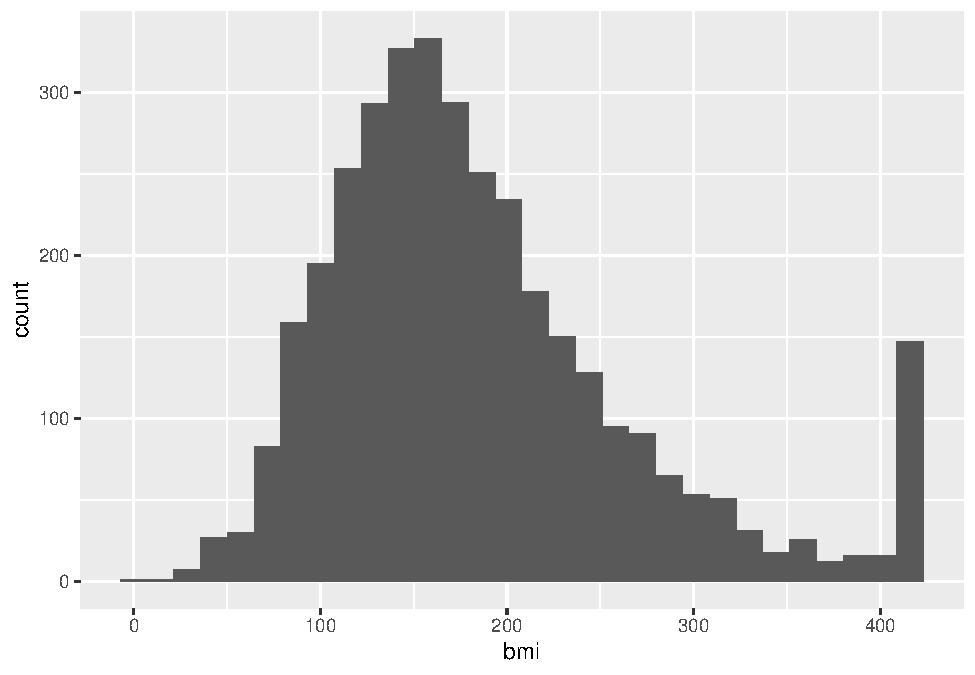
\includegraphics{_main_files/figure-latex/unnamed-chunk-95-1.pdf}

Staticians commonly prefer working with normally distributed data because this is a heavily studied and predictable distribution. Confirming that the variable is normally distributed opens up options for robust statistical approaches to be applied.

Is this heart dataset normally distributed?

QQ plots, or quantile-quantile plots, are unique scatterplots that help us determine the distribution. Rather than black and white diagnostic tool, this is a visualization tool for inform our analysis. The \texttt{qqnorm()} sorts the values in the vector and compares it to a theoretical normal distribution (the \texttt{norm} part of \texttt{qqnorm}).

\begin{Shaded}
\begin{Highlighting}[]
\FunctionTok{qqnorm}\NormalTok{(heart}\SpecialCharTok{$}\NormalTok{bmi)}
\end{Highlighting}
\end{Shaded}

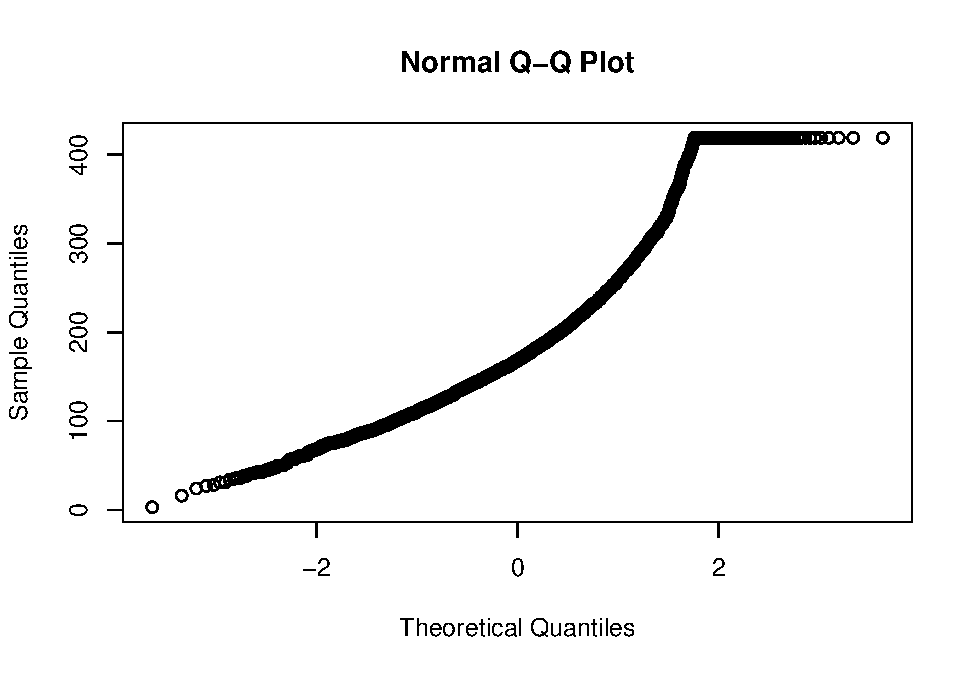
\includegraphics{_main_files/figure-latex/unnamed-chunk-96-1.pdf}

For a normal distribution, we ideally want a straight diagonal line. Notice the slight curve on the right end, we can see the tail is also on the right side of this histogram. Curves indicate deviation away from normality. This looks faily normal, we can check to see if a transformation improves the distribution.

\begin{Shaded}
\begin{Highlighting}[]
\FunctionTok{ggplot}\NormalTok{(heart, }\FunctionTok{aes}\NormalTok{(}\AttributeTok{x =} \FunctionTok{log2}\NormalTok{(bmi))) }\SpecialCharTok{+} 
  \FunctionTok{geom\_histogram}\NormalTok{()}
\end{Highlighting}
\end{Shaded}

\begin{verbatim}
## `stat_bin()` using `bins = 30`. Pick better value with `binwidth`.
\end{verbatim}

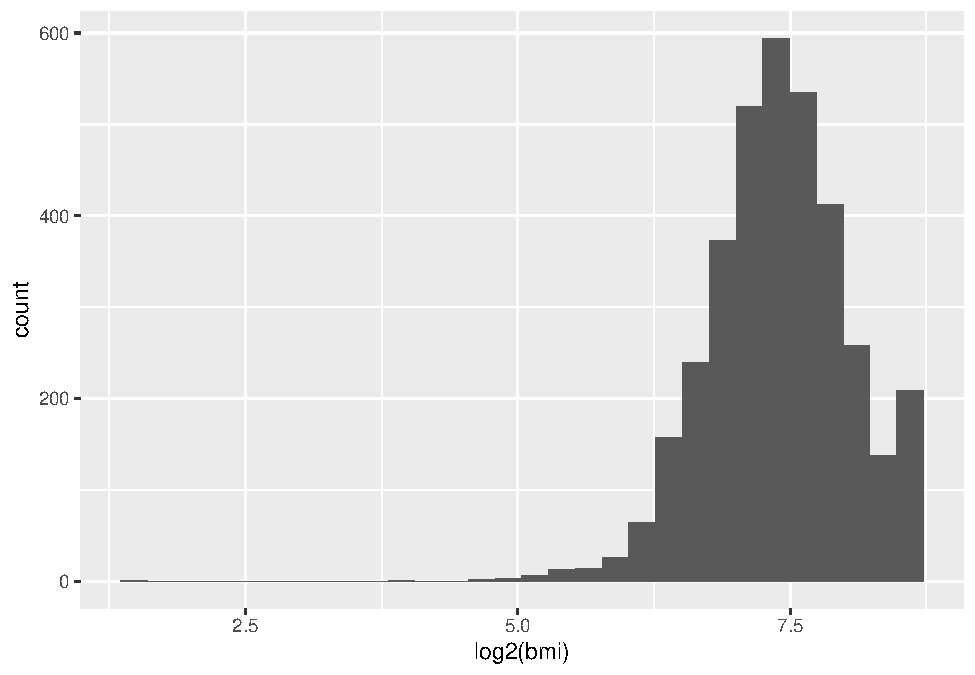
\includegraphics{_main_files/figure-latex/unnamed-chunk-97-1.pdf}

\begin{Shaded}
\begin{Highlighting}[]
\FunctionTok{qqnorm}\NormalTok{(}\FunctionTok{log2}\NormalTok{(heart}\SpecialCharTok{$}\NormalTok{bmi))}
\end{Highlighting}
\end{Shaded}

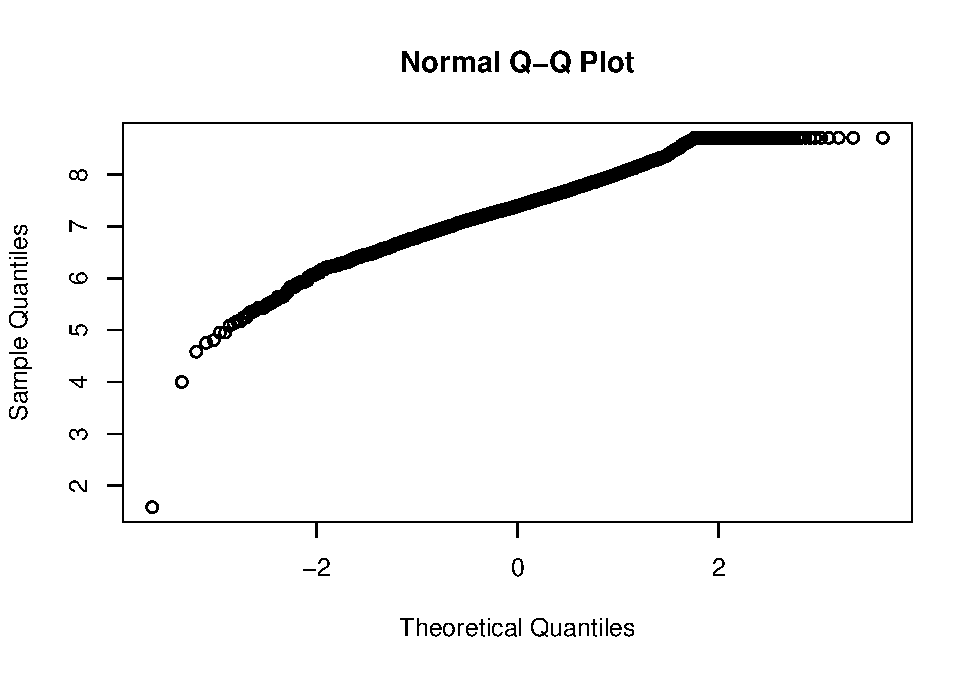
\includegraphics{_main_files/figure-latex/unnamed-chunk-97-2.pdf}

The tail is exaggerated. Since all transformations add some artificial noise, we avoid applying them when it does not significantly improve the shape of our data.

We will proceed with the non-transformed data.

\subsection{Linear Models}\label{linear-models}

Linear regression models allow us to investigate the relationship between two continuous variables. For simple linear models, we have one independent and one dependent variable. The independent variable is the one that is being controlled or manipulated in the experiment, and the dependent variable will change respectively.

For example, if we are investigating if a high fat diet affects sleep quality, the diet is the independent variable (changing or is different between participants) while the sleep quality is the dependent variable (depending on the diet, the sleep quality will change).

Here, we are investigating the relation between bmi and avg\_glucose\_level

We'll first visualize the two variables

\begin{Shaded}
\begin{Highlighting}[]
\FunctionTok{ggplot}\NormalTok{(heart)}\SpecialCharTok{+}
  \FunctionTok{geom\_point}\NormalTok{(}\FunctionTok{aes}\NormalTok{(}\AttributeTok{x=}\NormalTok{bmi, }\AttributeTok{y=}\NormalTok{avg\_glucose\_level, }\AttributeTok{alpha=}\FloatTok{0.3}\NormalTok{))}
\end{Highlighting}
\end{Shaded}

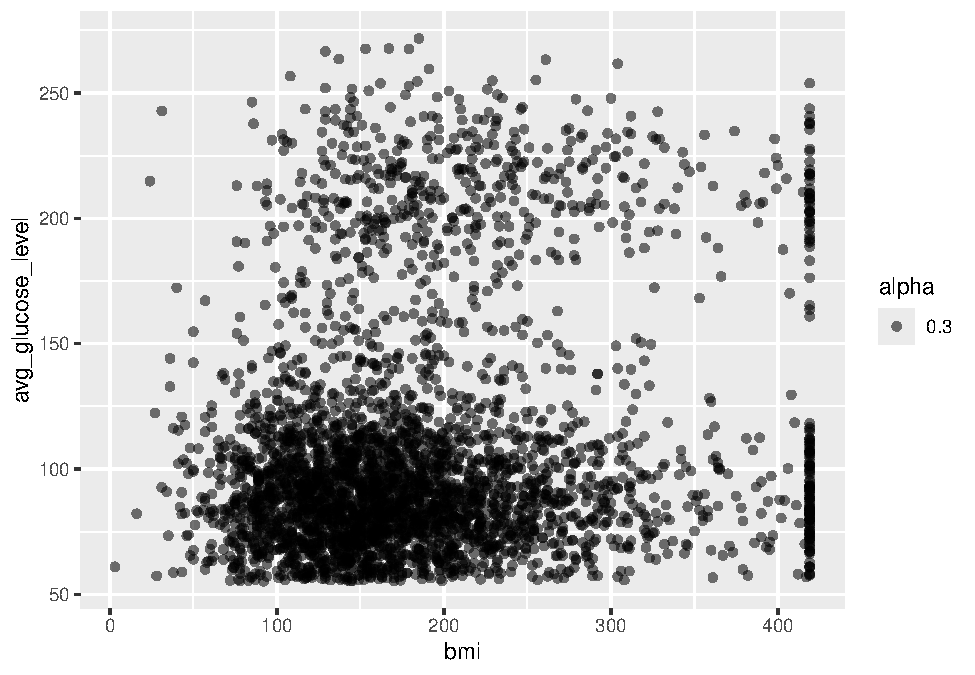
\includegraphics{_main_files/figure-latex/unnamed-chunk-98-1.pdf}

Notice here the aes is specified in the \texttt{geom\_point()} call rather than the parent \texttt{ggplot()} call. This is helpful if your plots have multiple layers and you want the aes to apply only to one layer. Parameters in the \texttt{ggplot()} call will apply to all layers in the plot where as parameters specified in the \texttt{geom\_point()} will only affect this specific layer.

For this plot with only one layer, this has no functional impact on the plot made, but this will be important if you make more complex and layered plots.

\begin{Shaded}
\begin{Highlighting}[]
\NormalTok{fit }\OtherTok{\textless{}{-}} \FunctionTok{lm}\NormalTok{(avg\_glucose\_level }\SpecialCharTok{\textasciitilde{}}\NormalTok{ bmi, }\AttributeTok{data =}\NormalTok{ heart)}
\end{Highlighting}
\end{Shaded}

This can be read as \texttt{avg\_glucose\_level} as a function of \texttt{bmi}

Use the function summary() on fit1 object to obtain more details of the model.

\begin{Shaded}
\begin{Highlighting}[]
\NormalTok{summary}
\end{Highlighting}
\end{Shaded}

\begin{verbatim}
## function (object, ...) 
## UseMethod("summary")
## <bytecode: 0x12849c3b8>
## <environment: namespace:base>
\end{verbatim}

This overall looks like a good model. The p-value is very low and statistically significant. However, the Multiple R-squared values is small and the slope of bmi is low.

From the results, we could conclude that changes in bmi are associated to the average glucose level as the p-value is less than 0.05. We can also state that as bmi increases, there will be an increase in the average glucose level as the slope is weakly positive 0.11.

Now that our model has given us the intercept and slope, we can use this information to build a formula in the format of

\begin{quote}
dependent = (m)(independent) + b
\end{quote}

\begin{quote}
avg\_glucose\_level = (0.097800)(bmi) + 90.823324
\end{quote}

We can use our knowledge of writing functions to calculate the predict the glucose level from the patient's bmi

\begin{Shaded}
\begin{Highlighting}[]
\NormalTok{calc\_gluc }\OtherTok{\textless{}{-}} \ControlFlowTok{function}\NormalTok{(bmi\_value) \{}
\NormalTok{  (}\FloatTok{0.097800}\SpecialCharTok{*}\NormalTok{bmi\_value) }\SpecialCharTok{+} \FloatTok{90.823324} \CommentTok{\# Change from brackets to * for multiply, bmi to bmi\_value}
\NormalTok{\}}

\NormalTok{heart[}\DecValTok{3}\NormalTok{, }\FunctionTok{c}\NormalTok{(}\StringTok{"bmi"}\NormalTok{, }\StringTok{"avg\_glucose\_level"}\NormalTok{)]}
\end{Highlighting}
\end{Shaded}

\begin{verbatim}
##   bmi avg_glucose_level
## 3 199            105.92
\end{verbatim}

\begin{Shaded}
\begin{Highlighting}[]
\FunctionTok{calc\_gluc}\NormalTok{(}\DecValTok{119}\NormalTok{)}
\end{Highlighting}
\end{Shaded}

\begin{verbatim}
## [1] 102.4615
\end{verbatim}

Next, let's visualize this using ggplot

\begin{Shaded}
\begin{Highlighting}[]
\CommentTok{\# Start with code from previous point plot }

\FunctionTok{ggplot}\NormalTok{(heart, }\FunctionTok{aes}\NormalTok{(}\AttributeTok{x=}\NormalTok{bmi, }\AttributeTok{y=}\NormalTok{avg\_glucose\_level, }\AttributeTok{alpha=}\FloatTok{0.3}\NormalTok{, }\AttributeTok{col =}\NormalTok{ stroke))}\SpecialCharTok{+}
  \FunctionTok{geom\_point}\NormalTok{() }\SpecialCharTok{+} \CommentTok{\# ADD PLUS SIGN}
  \FunctionTok{geom\_abline}\NormalTok{(}\AttributeTok{intercept =} \FloatTok{90.823324}\NormalTok{, }\AttributeTok{slope =} \FloatTok{0.097800}\NormalTok{, }\AttributeTok{color =} \StringTok{"purple"}\NormalTok{) }\CommentTok{\# ADD THIS LINE}
\end{Highlighting}
\end{Shaded}

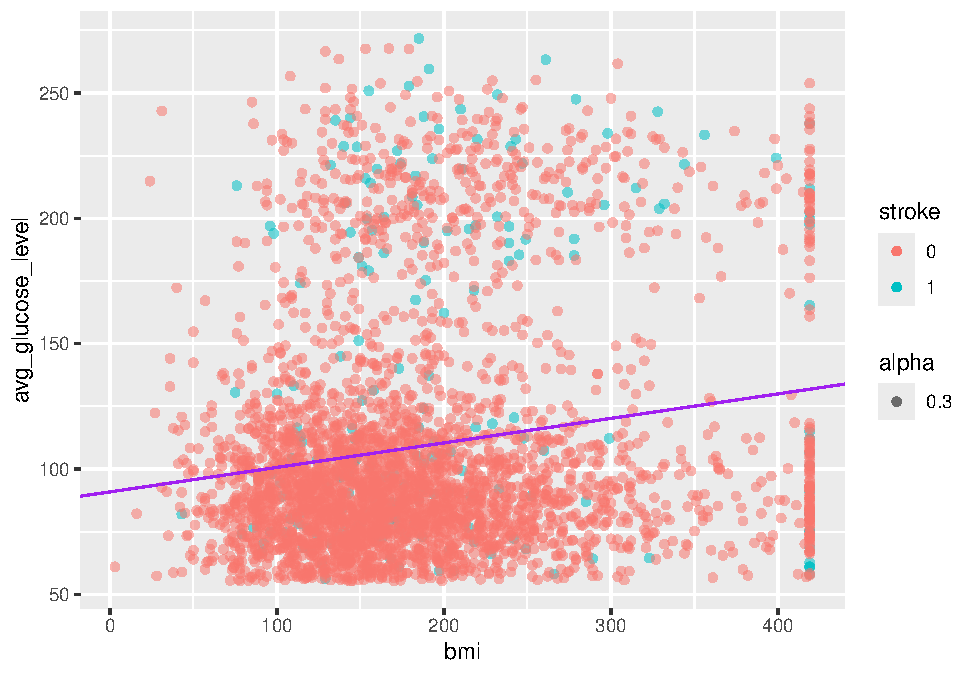
\includegraphics{_main_files/figure-latex/unnamed-chunk-102-1.pdf}

\subsection{Exercise}\label{exercise-9}

Hmm, this looks like there are two densities of data in this image. Let's try to investigate if we can figure it out.

I've started you off by creating two new objects, an object called \texttt{heart\_stroke} that contains only patents who experienced a stroke (stroke == 1) and a second object called \texttt{heart\_nostroke} that contains only patents who have not experienced a stroke (stroke == 0).

Next, create two separate linear models called \texttt{fit\_stroke} and \texttt{fit\_nostroke} - are they different? How will you visualize the data?

\begin{Shaded}
\begin{Highlighting}[]
\NormalTok{heart\_stroke }\OtherTok{\textless{}{-}} \FunctionTok{filter}\NormalTok{(heart, stroke }\SpecialCharTok{==} \DecValTok{1}\NormalTok{)}
\FunctionTok{table}\NormalTok{(heart\_stroke}\SpecialCharTok{$}\NormalTok{stroke)}
\end{Highlighting}
\end{Shaded}

\begin{verbatim}
## 
##   0   1 
##   0 202
\end{verbatim}

\begin{Shaded}
\begin{Highlighting}[]
\NormalTok{heart\_nostroke }\OtherTok{\textless{}{-}} \FunctionTok{filter}\NormalTok{(heart, stroke }\SpecialCharTok{==} \DecValTok{0}\NormalTok{)}
\FunctionTok{table}\NormalTok{(heart\_nostroke}\SpecialCharTok{$}\NormalTok{stroke)}
\end{Highlighting}
\end{Shaded}

\begin{verbatim}
## 
##    0    1 
## 3363    0
\end{verbatim}

\begin{Shaded}
\begin{Highlighting}[]
\CommentTok{\# From above: }
\CommentTok{\# fit \textless{}{-} lm(avg\_glucose\_level \textasciitilde{} bmi, data = heart)}

\NormalTok{fit\_stroke }\OtherTok{\textless{}{-}} \FunctionTok{lm}\NormalTok{(avg\_glucose\_level }\SpecialCharTok{\textasciitilde{}}\NormalTok{ bmi, }\AttributeTok{data =}\NormalTok{ heart\_stroke)}
\NormalTok{fit\_nostroke }\OtherTok{\textless{}{-}} \FunctionTok{lm}\NormalTok{(avg\_glucose\_level }\SpecialCharTok{\textasciitilde{}}\NormalTok{ bmi, }\AttributeTok{data =}\NormalTok{ heart\_nostroke)}

\FunctionTok{summary}\NormalTok{(fit\_stroke)}
\end{Highlighting}
\end{Shaded}

\begin{verbatim}
## 
## Call:
## lm(formula = avg_glucose_level ~ bmi, data = heart_stroke)
## 
## Residuals:
##    Min     1Q Median     3Q    Max 
## -92.34 -51.38 -27.21  60.90 138.98 
## 
## Coefficients:
##              Estimate Std. Error t value Pr(>|t|)    
## (Intercept) 118.92281   10.59306  11.226   <2e-16 ***
## bmi           0.07479    0.04670   1.602    0.111    
## ---
## Signif. codes:  0 '***' 0.001 '**' 0.01 '*' 0.05 '.' 0.1 ' ' 1
## 
## Residual standard error: 62.75 on 200 degrees of freedom
## Multiple R-squared:  0.01266,    Adjusted R-squared:  0.007726 
## F-statistic: 2.565 on 1 and 200 DF,  p-value: 0.1108
\end{verbatim}

\begin{Shaded}
\begin{Highlighting}[]
\FunctionTok{summary}\NormalTok{(fit\_nostroke)}
\end{Highlighting}
\end{Shaded}

\begin{verbatim}
## 
## Call:
## lm(formula = avg_glucose_level ~ bmi, data = heart_nostroke)
## 
## Residuals:
##    Min     1Q Median     3Q    Max 
## -72.67 -30.43 -13.96  10.36 164.40 
## 
## Coefficients:
##             Estimate Std. Error t value Pr(>|t|)    
## (Intercept) 89.92299    1.96082  45.860   <2e-16 ***
## bmi          0.09507    0.00972   9.781   <2e-16 ***
## ---
## Signif. codes:  0 '***' 0.001 '**' 0.01 '*' 0.05 '.' 0.1 ' ' 1
## 
## Residual standard error: 46.2 on 3361 degrees of freedom
## Multiple R-squared:  0.02768,    Adjusted R-squared:  0.02739 
## F-statistic: 95.68 on 1 and 3361 DF,  p-value: < 2.2e-16
\end{verbatim}

\begin{Shaded}
\begin{Highlighting}[]
\NormalTok{fit\_nostroke}\SpecialCharTok{$}\NormalTok{coefficients}
\end{Highlighting}
\end{Shaded}

\begin{verbatim}
## (Intercept)         bmi 
## 89.92298677  0.09507385
\end{verbatim}

\begin{Shaded}
\begin{Highlighting}[]
\FunctionTok{ggplot}\NormalTok{(heart, }\FunctionTok{aes}\NormalTok{(}\AttributeTok{x=}\NormalTok{bmi, }\AttributeTok{y=}\NormalTok{avg\_glucose\_level, }\AttributeTok{alpha=}\FloatTok{0.3}\NormalTok{, }\AttributeTok{col =}\NormalTok{ stroke))}\SpecialCharTok{+}
  \FunctionTok{geom\_point}\NormalTok{() }\SpecialCharTok{+} \CommentTok{\# ADD PLUS SIGN}
  \FunctionTok{geom\_abline}\NormalTok{(}\AttributeTok{intercept =} \FloatTok{90.823324}\NormalTok{, }\AttributeTok{slope =} \FloatTok{0.097800}\NormalTok{, }\AttributeTok{color =} \StringTok{"purple"}\NormalTok{) }\SpecialCharTok{+} 
  \FunctionTok{geom\_abline}\NormalTok{(}\AttributeTok{intercept =}\NormalTok{ fit\_nostroke}\SpecialCharTok{$}\NormalTok{coefficients[}\DecValTok{1}\NormalTok{], }\AttributeTok{slope =}\NormalTok{ fit\_nostroke}\SpecialCharTok{$}\NormalTok{coefficients[}\DecValTok{2}\NormalTok{], }\AttributeTok{color =} \StringTok{"red"}\NormalTok{) }\SpecialCharTok{+} 
  \FunctionTok{xlim}\NormalTok{(}\DecValTok{100}\NormalTok{, }\DecValTok{200}\NormalTok{)}\SpecialCharTok{+} 
  \FunctionTok{ylim}\NormalTok{(}\DecValTok{100}\NormalTok{, }\DecValTok{200}\NormalTok{)}
\end{Highlighting}
\end{Shaded}

\begin{verbatim}
## Warning: Removed 2951 rows containing missing values or values outside the scale range
## (`geom_point()`).
\end{verbatim}

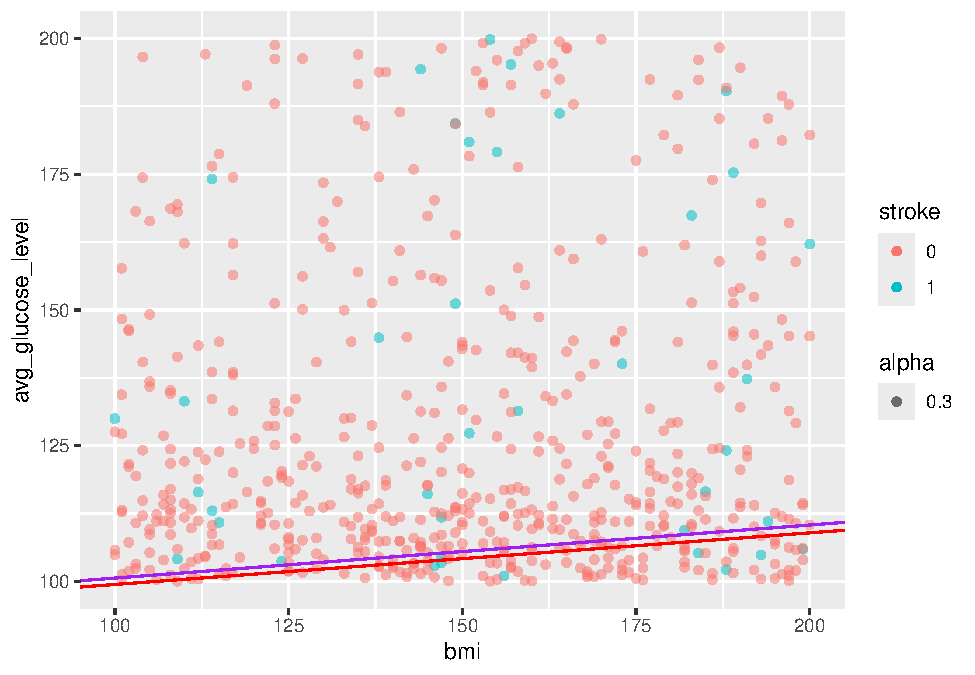
\includegraphics{_main_files/figure-latex/unnamed-chunk-104-1.pdf}

\subsection{Demo Detour to Function for lm Plots}\label{demo-detour-to-function-for-lm-plots}

\begin{Shaded}
\begin{Highlighting}[]
\CommentTok{\# The variables }
\NormalTok{which\_data }\OtherTok{\textless{}{-}}\NormalTok{ heart\_stroke}
\NormalTok{variable\_call }\OtherTok{\textless{}{-}} \StringTok{"avg\_glucose\_level \textasciitilde{} bmi"}
\NormalTok{custom\_col }\OtherTok{\textless{}{-}} \StringTok{"blue"}



\CommentTok{\# The actual task }

\NormalTok{lm\_gluc\_bmi }\OtherTok{\textless{}{-}} \ControlFlowTok{function}\NormalTok{(}\AttributeTok{which\_data =}\NormalTok{ heart\_stroke, }\AttributeTok{variable\_call =} \StringTok{"avg\_glucose\_level \textasciitilde{} bmi"}\NormalTok{, }\AttributeTok{custom\_col =} \StringTok{"blue"}\NormalTok{) \{}

  \CommentTok{\# Run liner model }
  
  \CommentTok{\# Make plot}

\NormalTok{fit\_stroke }\OtherTok{\textless{}{-}} \FunctionTok{lm}\NormalTok{(variable\_call, }\AttributeTok{data =}\NormalTok{ which\_data)}

\FunctionTok{ggplot}\NormalTok{(heart, }\FunctionTok{aes}\NormalTok{(}\AttributeTok{x=}\NormalTok{bmi, }\AttributeTok{y=}\NormalTok{avg\_glucose\_level, }\AttributeTok{alpha=}\FloatTok{0.3}\NormalTok{, }\AttributeTok{col =}\NormalTok{ stroke))}\SpecialCharTok{+}
  \FunctionTok{geom\_point}\NormalTok{() }\SpecialCharTok{+} \CommentTok{\# ADD PLUS SIGN}
  \FunctionTok{geom\_abline}\NormalTok{(}\AttributeTok{intercept =}\NormalTok{ fit\_nostroke}\SpecialCharTok{$}\NormalTok{coefficients[}\DecValTok{1}\NormalTok{], }\AttributeTok{slope =}\NormalTok{ fit\_nostroke}\SpecialCharTok{$}\NormalTok{coefficients[}\DecValTok{2}\NormalTok{], }\AttributeTok{color =}\NormalTok{ custom\_col)}

\NormalTok{\}}

\FunctionTok{lm\_gluc\_bmi}\NormalTok{(}\AttributeTok{custom\_col =} \StringTok{"green3"}\NormalTok{)}
\end{Highlighting}
\end{Shaded}

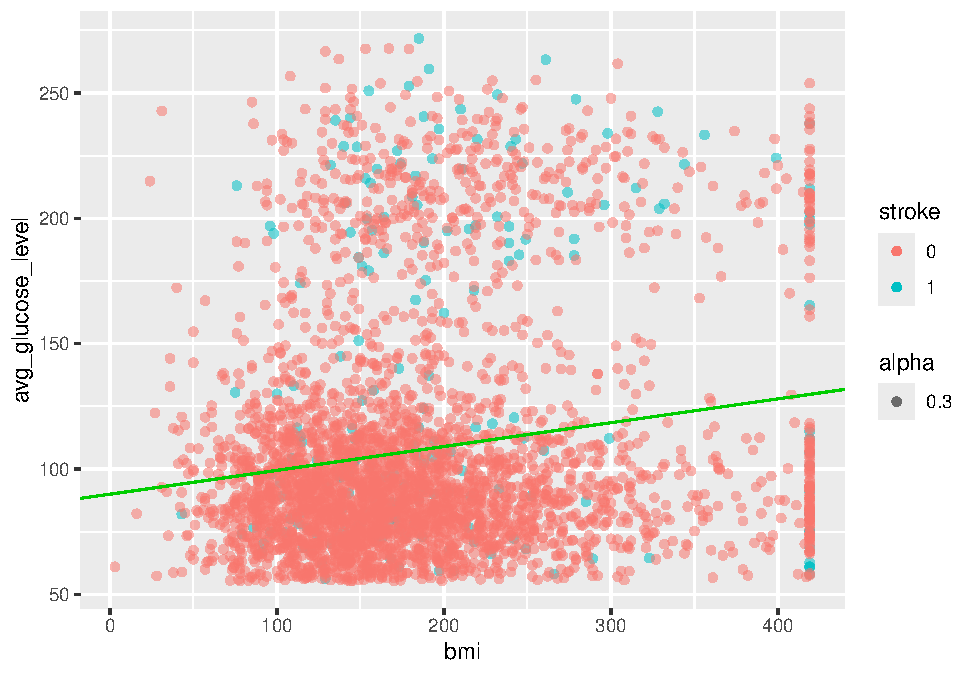
\includegraphics{_main_files/figure-latex/unnamed-chunk-105-1.pdf}

\subsection{Notes on Data Types}\label{notes-on-data-types}

Numeric
-dbl doublets, int integers

Character
-char or fact factor
- characters are independent words
- factors have relations between identical entries

-categorical
- require factor

Logical

\begin{quote}
\begin{quote}
Differences are apparent when using a summary call
\end{quote}
\end{quote}

\subsection{Day 2 Project}\label{day-2-project}

For this mini guided project, we will be working with a dataset that contains the prices and other attributes of almost 54,000 diamonds and is publicly available at: \url{https://www.kaggle.com/datasets/shivam2503/diamonds}

Here is some more information about each column:

price price in US dollars (\$326--\$18,823)
carat weight of the diamond (0.2--5.01)
cut quality of the cut (Fair, Good, Very Good, Premium, Ideal)
color diamond colour, from J (worst) to D (best)
clarity a measurement of how clear the diamond is (I1 (worst), SI2, SI1, VS2, VS1, VVS2, VVS1, IF (best))
x length in mm (0--10.74)
y width in mm (0--58.9)
z depth in mm (0--31.8)
depth total depth percentage = z / mean(x, y) = 2 * z / (x + y) (43--79)
table width of top of diamond relative to widest point (43--95)

Insert a code chunk underneath each step to carry out the instruction.

\begin{enumerate}
\def\labelenumi{\arabic{enumi}.}
\tightlist
\item
  Read in the ``diamonds.csv'' data into an object called data. Use the \texttt{strongAsFactors} parameter to automatically import the character values as a factor. Check the object you created by printing out the first 10 rows and applying the summary function.
\end{enumerate}

\begin{Shaded}
\begin{Highlighting}[]
\NormalTok{diamonds }\OtherTok{\textless{}{-}} \FunctionTok{read.csv}\NormalTok{(}\StringTok{"../INR{-}2024/datasets/diamonds.csv"}\NormalTok{, }\AttributeTok{header =}\NormalTok{ T, }\AttributeTok{stringsAsFactors =}\NormalTok{ T)}

\FunctionTok{head}\NormalTok{(diamonds)}
\end{Highlighting}
\end{Shaded}

\begin{verbatim}
##   X carat       cut color clarity depth table price    x    y    z
## 1 1  0.23     Ideal     E     SI2  61.5    55   326 3.95 3.98 2.43
## 2 2  0.21   Premium     E     SI1  59.8    61   326 3.89 3.84 2.31
## 3 3  0.23      Good     E     VS1  56.9    65   327 4.05 4.07 2.31
## 4 4  0.29   Premium     I     VS2  62.4    58   334 4.20 4.23 2.63
## 5 5  0.31      Good     J     SI2  63.3    58   335 4.34 4.35 2.75
## 6 6  0.24 Very Good     J    VVS2  62.8    57   336 3.94 3.96 2.48
\end{verbatim}

\begin{Shaded}
\begin{Highlighting}[]
\FunctionTok{summary}\NormalTok{(diamonds)}
\end{Highlighting}
\end{Shaded}

\begin{verbatim}
##        X             carat               cut        color        clarity     
##  Min.   :    1   Min.   :0.2000   Fair     : 1610   D: 6775   SI1    :13065  
##  1st Qu.:13486   1st Qu.:0.4000   Good     : 4906   E: 9797   VS2    :12258  
##  Median :26970   Median :0.7000   Ideal    :21551   F: 9542   SI2    : 9194  
##  Mean   :26970   Mean   :0.7979   Premium  :13791   G:11292   VS1    : 8171  
##  3rd Qu.:40455   3rd Qu.:1.0400   Very Good:12082   H: 8304   VVS2   : 5066  
##  Max.   :53940   Max.   :5.0100                     I: 5422   VVS1   : 3655  
##                                                     J: 2808   (Other): 2531  
##      depth           table           price             x         
##  Min.   :43.00   Min.   :43.00   Min.   :  326   Min.   : 0.000  
##  1st Qu.:61.00   1st Qu.:56.00   1st Qu.:  950   1st Qu.: 4.710  
##  Median :61.80   Median :57.00   Median : 2401   Median : 5.700  
##  Mean   :61.75   Mean   :57.46   Mean   : 3933   Mean   : 5.731  
##  3rd Qu.:62.50   3rd Qu.:59.00   3rd Qu.: 5324   3rd Qu.: 6.540  
##  Max.   :79.00   Max.   :95.00   Max.   :18823   Max.   :10.740  
##                                                                  
##        y                z         
##  Min.   : 0.000   Min.   : 0.000  
##  1st Qu.: 4.720   1st Qu.: 2.910  
##  Median : 5.710   Median : 3.530  
##  Mean   : 5.735   Mean   : 3.539  
##  3rd Qu.: 6.540   3rd Qu.: 4.040  
##  Max.   :58.900   Max.   :31.800  
## 
\end{verbatim}

\begin{enumerate}
\def\labelenumi{\arabic{enumi}.}
\setcounter{enumi}{1}
\tightlist
\item
  We'll start investigating the relationship between different variables with price. Create a boxplot using ggplot with the cut on the x axis and the price on the y axis.
\end{enumerate}

\begin{Shaded}
\begin{Highlighting}[]
\FunctionTok{ggplot}\NormalTok{(}\AttributeTok{data =}\NormalTok{ diamonds, }\FunctionTok{aes}\NormalTok{(}\AttributeTok{x =}\NormalTok{ cut, }\AttributeTok{y =}\NormalTok{ price)) }\SpecialCharTok{+} 
  \FunctionTok{geom\_boxplot}\NormalTok{()}
\end{Highlighting}
\end{Shaded}

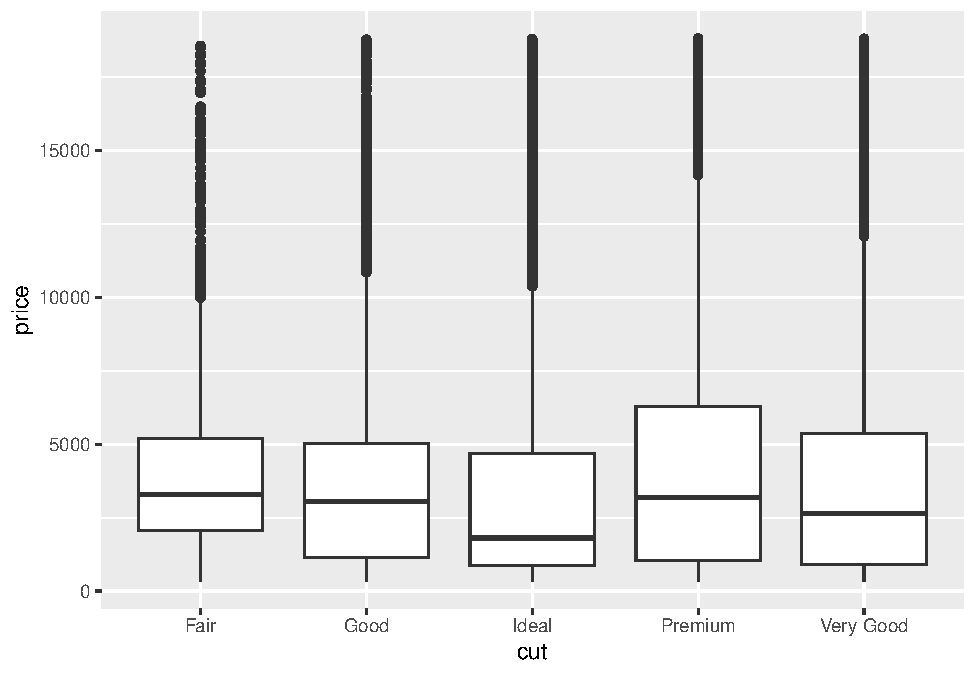
\includegraphics{_main_files/figure-latex/unnamed-chunk-107-1.pdf}

\begin{enumerate}
\def\labelenumi{\arabic{enumi}.}
\setcounter{enumi}{2}
\tightlist
\item
  Using the code in the previous step as foundation, create an object called \texttt{diamonds\_categorical} that contains the name of all the categorical columns. Then, write a loop to print out a separate plot with each of the different categorical variables on the x axis and price on the y-axis.
\end{enumerate}

Remember how aes can be specified in both the \texttt{ggplot()} or \texttt{geom\_xx()} layer? You will need to use this because we are string the name of a column as a variable in our loop and in order for R to know that it is looking for a column name rather than an object, you will need to use the \texttt{aes\_string()} parameter for just the \texttt{geom\_boxplot()} layer to specify the changing x axis. The y axis can remain with \texttt{aes()} in the parent \texttt{ggplot()} layer.

\begin{Shaded}
\begin{Highlighting}[]
\FunctionTok{str}\NormalTok{(diamonds)}
\end{Highlighting}
\end{Shaded}

\begin{verbatim}
## 'data.frame':    53940 obs. of  11 variables:
##  $ X      : int  1 2 3 4 5 6 7 8 9 10 ...
##  $ carat  : num  0.23 0.21 0.23 0.29 0.31 0.24 0.24 0.26 0.22 0.23 ...
##  $ cut    : Factor w/ 5 levels "Fair","Good",..: 3 4 2 4 2 5 5 5 1 5 ...
##  $ color  : Factor w/ 7 levels "D","E","F","G",..: 2 2 2 6 7 7 6 5 2 5 ...
##  $ clarity: Factor w/ 8 levels "I1","IF","SI1",..: 4 3 5 6 4 8 7 3 6 5 ...
##  $ depth  : num  61.5 59.8 56.9 62.4 63.3 62.8 62.3 61.9 65.1 59.4 ...
##  $ table  : num  55 61 65 58 58 57 57 55 61 61 ...
##  $ price  : int  326 326 327 334 335 336 336 337 337 338 ...
##  $ x      : num  3.95 3.89 4.05 4.2 4.34 3.94 3.95 4.07 3.87 4 ...
##  $ y      : num  3.98 3.84 4.07 4.23 4.35 3.96 3.98 4.11 3.78 4.05 ...
##  $ z      : num  2.43 2.31 2.31 2.63 2.75 2.48 2.47 2.53 2.49 2.39 ...
\end{verbatim}

\begin{Shaded}
\begin{Highlighting}[]
\NormalTok{diamonds\_categorical }\OtherTok{\textless{}{-}} \FunctionTok{c}\NormalTok{(}\StringTok{"cut"}\NormalTok{, }\StringTok{"color"}\NormalTok{, }\StringTok{"clarity"}\NormalTok{)}

\ControlFlowTok{for}\NormalTok{(cat }\ControlFlowTok{in}\NormalTok{ diamonds\_categorical) \{}
\NormalTok{  diaplot }\OtherTok{\textless{}{-}} \FunctionTok{ggplot}\NormalTok{(}\AttributeTok{data =}\NormalTok{ diamonds, }\FunctionTok{aes}\NormalTok{(}\AttributeTok{y =}\NormalTok{ price)) }\SpecialCharTok{+} 
    \FunctionTok{geom\_boxplot}\NormalTok{(}\FunctionTok{aes\_string}\NormalTok{(}\AttributeTok{x =}\NormalTok{ cat))}
  
  \FunctionTok{print}\NormalTok{(diaplot)}
\NormalTok{\}}
\end{Highlighting}
\end{Shaded}

\begin{verbatim}
## Warning: `aes_string()` was deprecated in ggplot2 3.0.0.
## i Please use tidy evaluation idioms with `aes()`.
## i See also `vignette("ggplot2-in-packages")` for more information.
## This warning is displayed once every 8 hours.
## Call `lifecycle::last_lifecycle_warnings()` to see where this warning was
## generated.
\end{verbatim}

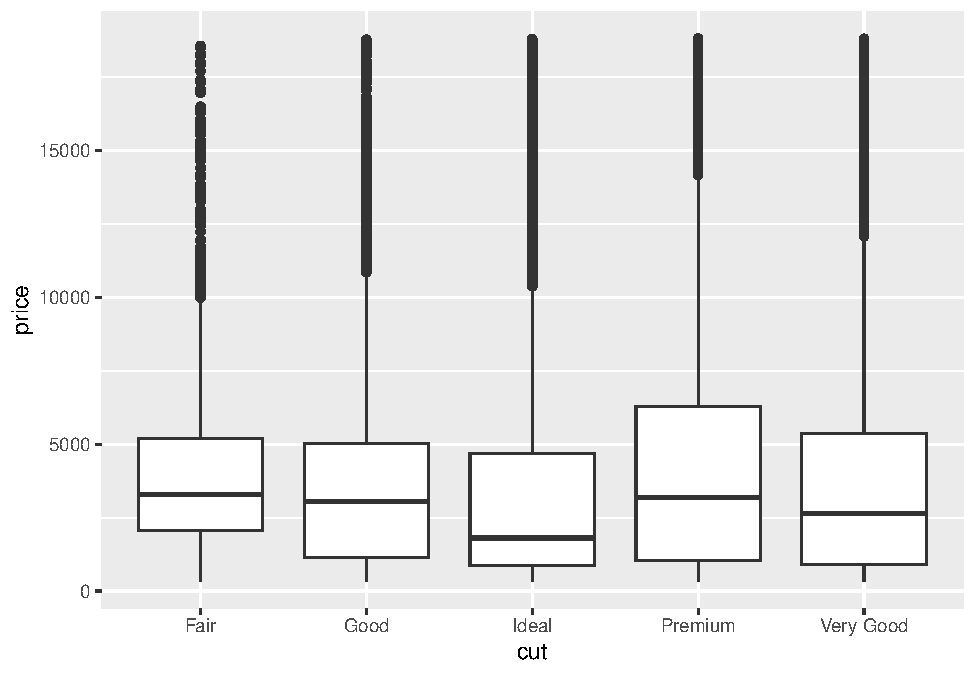
\includegraphics{_main_files/figure-latex/unnamed-chunk-108-1.pdf} 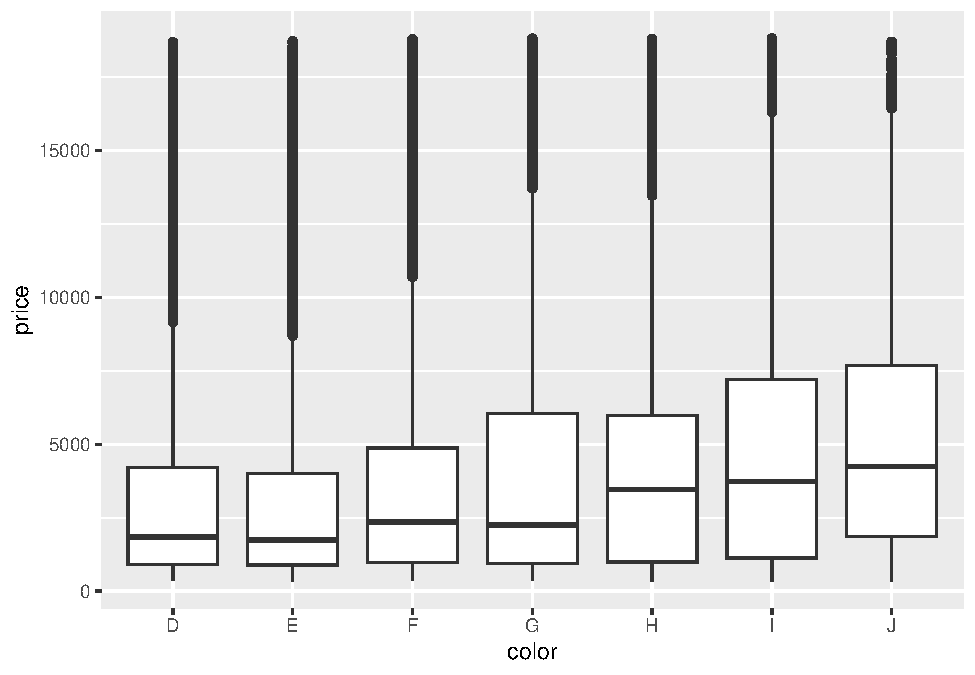
\includegraphics{_main_files/figure-latex/unnamed-chunk-108-2.pdf} 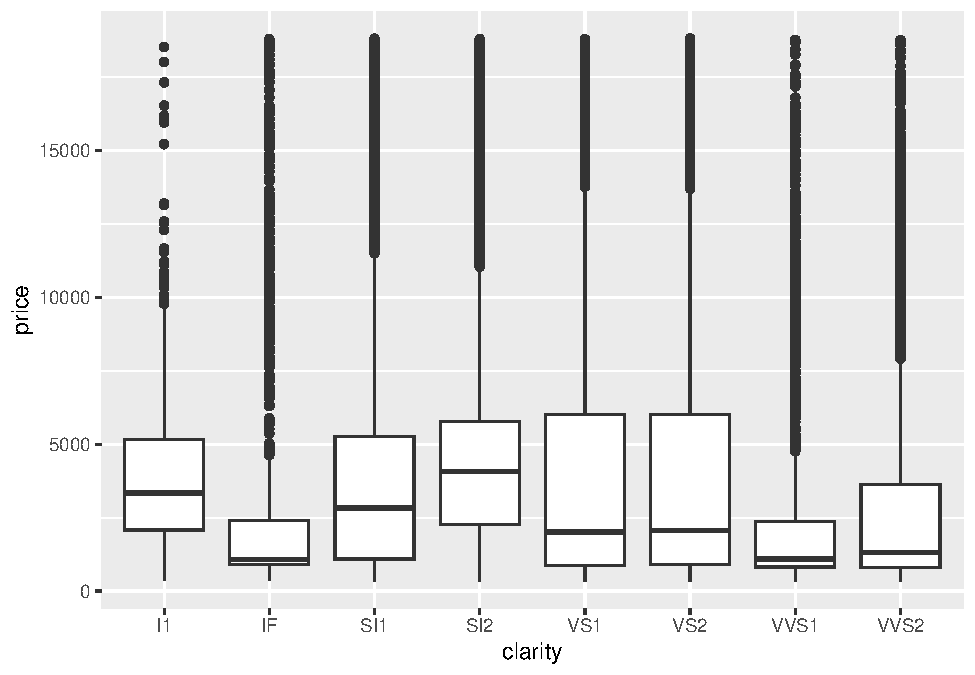
\includegraphics{_main_files/figure-latex/unnamed-chunk-108-3.pdf}

\begin{enumerate}
\def\labelenumi{\arabic{enumi}.}
\setcounter{enumi}{3}
\tightlist
\item
  Write a function called \texttt{diamond\_continous} that allows you to make a scatterplot that accepts one variable to plot on the x-axis as well as another variable to color the plot by as the inputs. Price will remain on the y-axis.
\end{enumerate}

Start out by making one plot, make it generalized, and then convert this into a function.

\begin{Shaded}
\begin{Highlighting}[]
\NormalTok{diamond\_continous }\OtherTok{\textless{}{-}} \ControlFlowTok{function}\NormalTok{(contV, colV) \{}
  
\NormalTok{  diaPlot }\OtherTok{\textless{}{-}} \FunctionTok{ggplot}\NormalTok{(}\AttributeTok{data =}\NormalTok{ diamonds, }\FunctionTok{aes}\NormalTok{(}\AttributeTok{y =}\NormalTok{ price)) }\SpecialCharTok{+} 
    \FunctionTok{geom\_point}\NormalTok{(}\FunctionTok{aes\_string}\NormalTok{(}\AttributeTok{x =}\NormalTok{ contV, }\AttributeTok{color =}\NormalTok{ colV), }\AttributeTok{alpha =} \FloatTok{0.4}\NormalTok{)}
  
  \FunctionTok{print}\NormalTok{(diaPlot)}
  
\NormalTok{\}}

\FunctionTok{diamond\_continous}\NormalTok{(}\StringTok{"carat"}\NormalTok{, }\StringTok{"clarity"}\NormalTok{)}
\end{Highlighting}
\end{Shaded}

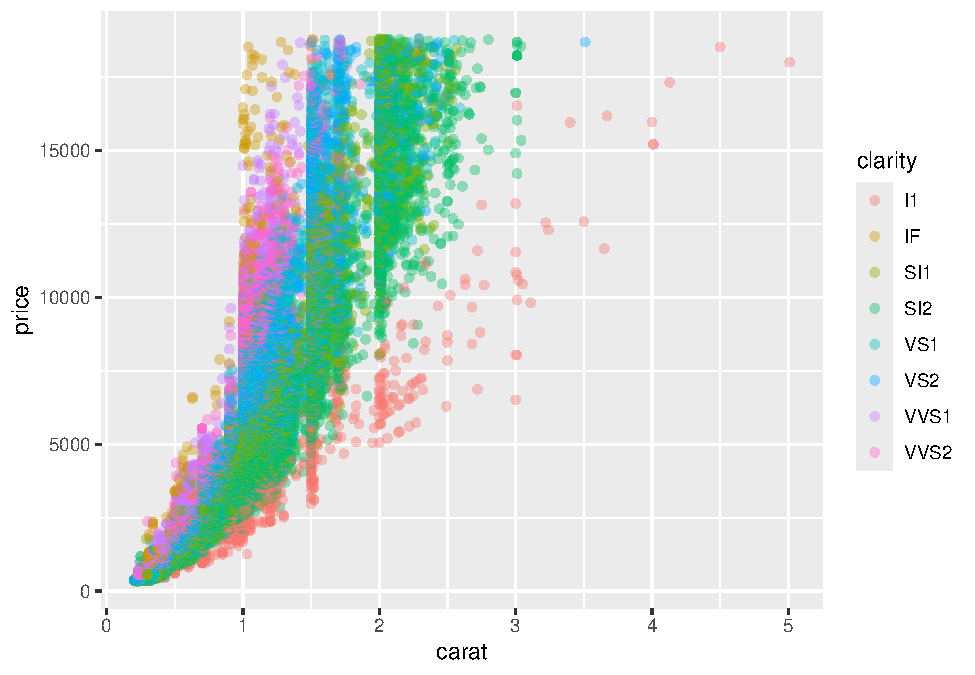
\includegraphics{_main_files/figure-latex/unnamed-chunk-109-1.pdf}

\begin{enumerate}
\def\labelenumi{\arabic{enumi}.}
\setcounter{enumi}{4}
\tightlist
\item
  Based on your plots from the previous step, pick a continuous variable to compare with price and create a linear model. Make sure the price is the dependent variable. Add a layer to your plot generated by the function to include the equation of the line.
\end{enumerate}

Is the relationship significant?

\begin{Shaded}
\begin{Highlighting}[]
\NormalTok{fit\_diamond }\OtherTok{\textless{}{-}} \FunctionTok{lm}\NormalTok{(price }\SpecialCharTok{\textasciitilde{}}\NormalTok{ carat, }\AttributeTok{data =}\NormalTok{ diamonds)}

\NormalTok{fit\_diamond}\SpecialCharTok{$}\NormalTok{coefficients}
\end{Highlighting}
\end{Shaded}

\begin{verbatim}
## (Intercept)       carat 
##   -2256.361    7756.426
\end{verbatim}

\begin{Shaded}
\begin{Highlighting}[]
\FunctionTok{diamond\_continous}\NormalTok{(}\StringTok{"carat"}\NormalTok{, }\StringTok{"clarity"}\NormalTok{) }\SpecialCharTok{+} 
  \FunctionTok{geom\_abline}\NormalTok{(}\AttributeTok{intercept =}\NormalTok{ fit\_diamond}\SpecialCharTok{$}\NormalTok{coefficients[}\DecValTok{1}\NormalTok{], }\AttributeTok{slope =}\NormalTok{ fit\_diamond}\SpecialCharTok{$}\NormalTok{coefficients[}\DecValTok{2}\NormalTok{], }\AttributeTok{color =} \StringTok{"red"}\NormalTok{, }\AttributeTok{size =} \DecValTok{2}\NormalTok{) }
\end{Highlighting}
\end{Shaded}

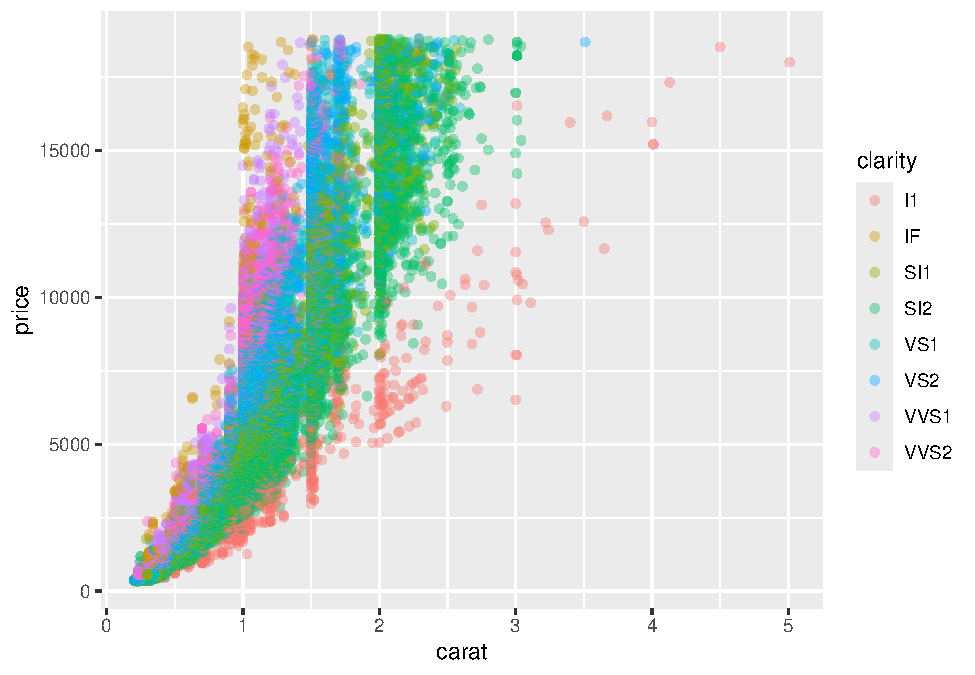
\includegraphics{_main_files/figure-latex/unnamed-chunk-110-1.pdf}

\begin{verbatim}
## Warning: Using `size` aesthetic for lines was deprecated in ggplot2 3.4.0.
## i Please use `linewidth` instead.
## This warning is displayed once every 8 hours.
## Call `lifecycle::last_lifecycle_warnings()` to see where this warning was
## generated.
\end{verbatim}

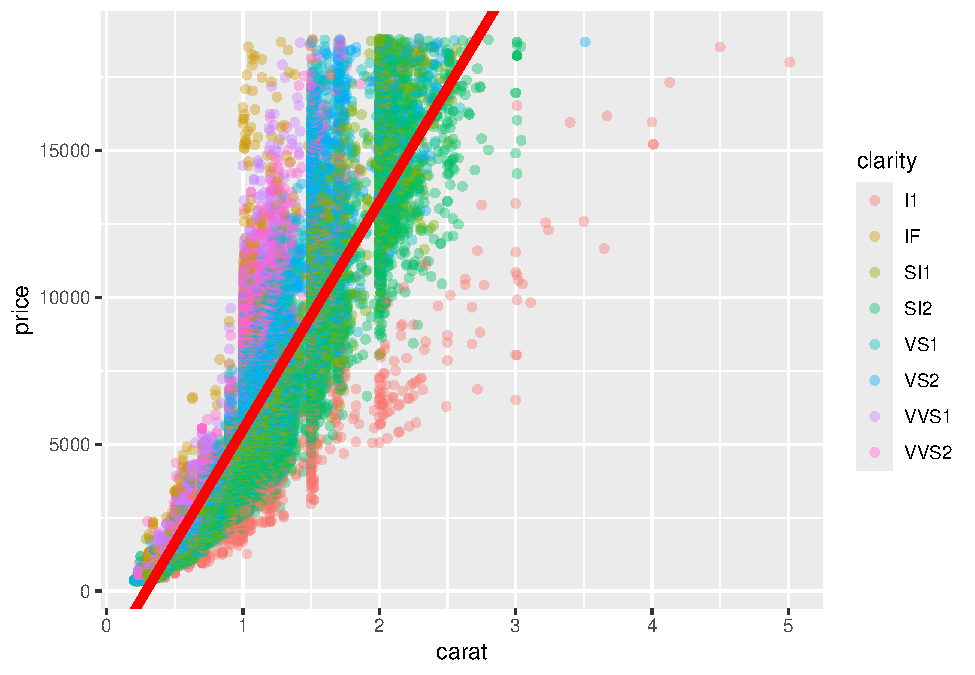
\includegraphics{_main_files/figure-latex/unnamed-chunk-110-2.pdf}

Congratulations! You have completed Lab 2!

  \bibliography{book.bib,packages.bib}

\end{document}
